\documentclass[a4paper]{book}
\usepackage{makeidx}
\usepackage{graphicx}
\usepackage{multicol}
\usepackage{float}
\usepackage{listings}
\usepackage{color}
\usepackage{ifthen}
\usepackage[table]{xcolor}
\usepackage{textcomp}
\usepackage{alltt}
\usepackage{ifpdf}
\ifpdf
\usepackage[pdftex,
            pagebackref=true,
            colorlinks=true,
            linkcolor=blue,
            unicode
           ]{hyperref}
\else
\usepackage[ps2pdf,
            pagebackref=true,
            colorlinks=true,
            linkcolor=blue,
            unicode
           ]{hyperref}
\usepackage{pspicture}
\fi
\usepackage[utf8]{inputenc}
\usepackage{mathptmx}
\usepackage[scaled=.90]{helvet}
\usepackage{courier}
\usepackage{doxygen}
\lstset{language=C++,inputencoding=utf8,basicstyle=\footnotesize,breaklines=true,breakatwhitespace=true,tabsize=4,numbers=left }
\makeindex
\setcounter{tocdepth}{3}
\renewcommand{\footrulewidth}{0.4pt}
\begin{document}
\hypersetup{pageanchor=false}
\begin{titlepage}
\vspace*{7cm}
\begin{center}
{\Large libchessengine \\[1ex]\large 0.2.1 }\\
\vspace*{1cm}
{\large Generated by Doxygen 1.7.3}\\
\vspace*{0.5cm}
{\small Tue May 31 2011 02:45:37}\\
\end{center}
\end{titlepage}
\clearemptydoublepage
\pagenumbering{roman}
\tableofcontents
\clearemptydoublepage
\pagenumbering{arabic}
\hypersetup{pageanchor=true}
\chapter{README}
\label{README}
\hypertarget{README}{}
\hypertarget{README_About}{}\section{About}\label{README_About}
libchessengine -\/ Parse PGN files, make moves from an game in input PGN file, print game, move, table to stream like std::ostream ( for example std::cout ) Uses modified pgnlib for parse PGN files\hypertarget{README_pgnlib}{}\section{Library}\label{README_pgnlib}
Compile, decompile chess games from/to $\ast$.pgn files. \href{http:}{\tt http:}//en.wikipedia.com/PGN\_\-Notation Uses GNU GPL library. Original source: \href{http://sourceforge.net/projects/pgnlib}{\tt http://sourceforge.net/projects/pgnlib}\hypertarget{README__inst_}{}\section{Installation Chess engine}\label{README__inst_}
\begin{DoxyNote}{Note}
Install libpgn first (\hyperlink{README__lpgninst_}{libpgn Installation}), then instal libchessengine make 
\end{DoxyNote}
sudo make install \hypertarget{README__lpgninst_}{}\subsection{libpgn Installation}\label{README__lpgninst_}
./configure make sudo make install \hypertarget{README_Using}{}\section{Using}\label{README_Using}
First \hyperlink{README__inst_}{Installation Chess engine} This library can be build as static library and/or shared object \begin{DoxySeeAlso}{See also}
examples 
\end{DoxySeeAlso}

\chapter{Namespace Index}
\section{Namespace List}
Here is a list of all documented namespaces with brief descriptions:\begin{DoxyCompactList}
\item\contentsline{section}{\hyperlink{namespaceChEngn}{ChEngn} (Contains all typedefs, constants, classes defined in )}{\pageref{namespaceChEngn}}{}
\end{DoxyCompactList}

\chapter{Class Index}
\section{Class Hierarchy}
This inheritance list is sorted roughly, but not completely, alphabetically:\begin{DoxyCompactList}
\item \contentsline{section}{pgn::bad\_\-pgn\_\-file}{\pageref{classpgn_1_1bad__pgn__file}}{}
\item \contentsline{section}{ChEngn::BadMove}{\pageref{classChEngn_1_1BadMove}}{}
\item \contentsline{section}{pgn::CommentText}{\pageref{classpgn_1_1CommentText}}{}
\item \contentsline{section}{ChEngn::Engine}{\pageref{classChEngn_1_1Engine}}{}
\item \contentsline{section}{ChEngn::Enumerator}{\pageref{classChEngn_1_1Enumerator}}{}
\item \contentsline{section}{pgn::File}{\pageref{classpgn_1_1File}}{}
\item \contentsline{section}{pgn::Game}{\pageref{classpgn_1_1Game}}{}
\item \contentsline{section}{pgn::GameCollection}{\pageref{classpgn_1_1GameCollection}}{}
\item \contentsline{section}{pgn::GameResult}{\pageref{classpgn_1_1GameResult}}{}
\item \contentsline{section}{pgn::TagList::iterator}{\pageref{classpgn_1_1TagList_1_1iterator}}{}
\item \contentsline{section}{pgn::GameCollection::iterator}{\pageref{classpgn_1_1GameCollection_1_1iterator}}{}
\item \contentsline{section}{pgn::MoveList::iterator}{\pageref{classpgn_1_1MoveList_1_1iterator}}{}
\item \contentsline{section}{ChEngn::Move}{\pageref{classChEngn_1_1Move}}{}
\begin{DoxyCompactList}
\item \contentsline{section}{ChEngn::KnightMove}{\pageref{classChEngn_1_1KnightMove}}{}
\item \contentsline{section}{ChEngn::PawnMove}{\pageref{classChEngn_1_1PawnMove}}{}
\end{DoxyCompactList}
\item \contentsline{section}{pgn::Move}{\pageref{classpgn_1_1Move}}{}
\item \contentsline{section}{pgn::MoveList}{\pageref{classpgn_1_1MoveList}}{}
\item \contentsline{section}{pgn::parse\_\-exception}{\pageref{classpgn_1_1parse__exception}}{}
\begin{DoxyCompactList}
\item \contentsline{section}{pgn::invalid\_\-castle\_\-string}{\pageref{classpgn_1_1invalid__castle__string}}{}
\item \contentsline{section}{pgn::invalid\_\-ply\_\-text}{\pageref{classpgn_1_1invalid__ply__text}}{}
\item \contentsline{section}{pgn::invalid\_\-result}{\pageref{classpgn_1_1invalid__result}}{}
\item \contentsline{section}{pgn::invalid\_\-tag}{\pageref{classpgn_1_1invalid__tag}}{}
\item \contentsline{section}{pgn::missing\_\-result}{\pageref{classpgn_1_1missing__result}}{}
\item \contentsline{section}{pgn::unsupported\_\-glyphs}{\pageref{classpgn_1_1unsupported__glyphs}}{}
\item \contentsline{section}{pgn::unsupported\_\-variations}{\pageref{classpgn_1_1unsupported__variations}}{}
\end{DoxyCompactList}
\item \contentsline{section}{pgn::Parser}{\pageref{classpgn_1_1Parser}}{}
\item \contentsline{section}{pgn::Piece}{\pageref{classpgn_1_1Piece}}{}
\item \contentsline{section}{ChEngn::Piece}{\pageref{classChEngn_1_1Piece}}{}
\item \contentsline{section}{pgn::Ply}{\pageref{classpgn_1_1Ply}}{}
\item \contentsline{section}{pgn::Square}{\pageref{classpgn_1_1Square}}{}
\item \contentsline{section}{ChEngn::Table}{\pageref{classChEngn_1_1Table}}{}
\item \contentsline{section}{pgn::Tag}{\pageref{classpgn_1_1Tag}}{}
\item \contentsline{section}{pgn::TagList}{\pageref{classpgn_1_1TagList}}{}
\end{DoxyCompactList}

\chapter{Class Index}
\section{Class List}
Here are the classes, structs, unions and interfaces with brief descriptions:\begin{DoxyCompactList}
\item\contentsline{section}{\hyperlink{classpgn_1_1bad__pgn__file}{pgn::bad\_\-pgn\_\-file} (Throws when file in incorrect/invalid )}{\pageref{classpgn_1_1bad__pgn__file}}{}
\item\contentsline{section}{\hyperlink{classChEngn_1_1BadMove}{ChEngn::BadMove} (Implements all exception which will be generated ty \hyperlink{classChEngn_1_1Engine}{ChEngn::Engine} while trying to make move which i sincorrect )}{\pageref{classChEngn_1_1BadMove}}{}
\item\contentsline{section}{\hyperlink{classpgn_1_1CommentText}{pgn::CommentText} (Provides comment to move )}{\pageref{classpgn_1_1CommentText}}{}
\item\contentsline{section}{\hyperlink{classChEngn_1_1Engine}{ChEngn::Engine} (Make moves )}{\pageref{classChEngn_1_1Engine}}{}
\item\contentsline{section}{\hyperlink{classChEngn_1_1Enumerator}{ChEngn::Enumerator} (Enumerate possibile moves )}{\pageref{classChEngn_1_1Enumerator}}{}
\item\contentsline{section}{\hyperlink{classpgn_1_1File}{pgn::File} (Opens and extract games from PGN file and/or compile \hyperlink{classpgn_1_1GameCollection}{pgn::GameCollection} fo file )}{\pageref{classpgn_1_1File}}{}
\item\contentsline{section}{\hyperlink{classpgn_1_1Game}{pgn::Game} (Represents information about game )}{\pageref{classpgn_1_1Game}}{}
\item\contentsline{section}{\hyperlink{classpgn_1_1GameCollection}{pgn::GameCollection} (Stores a collection of \hyperlink{classpgn_1_1Game}{pgn::Game} )}{\pageref{classpgn_1_1GameCollection}}{}
\item\contentsline{section}{\hyperlink{classpgn_1_1GameResult}{pgn::GameResult} (Stores information about game result )}{\pageref{classpgn_1_1GameResult}}{}
\item\contentsline{section}{\hyperlink{classpgn_1_1invalid__castle__string}{pgn::invalid\_\-castle\_\-string} (Throws when castle in pgnfile is incorrect format )}{\pageref{classpgn_1_1invalid__castle__string}}{}
\item\contentsline{section}{\hyperlink{classpgn_1_1invalid__ply__text}{pgn::invalid\_\-ply\_\-text} (Throws when ply is in incorrect format )}{\pageref{classpgn_1_1invalid__ply__text}}{}
\item\contentsline{section}{\hyperlink{classpgn_1_1invalid__result}{pgn::invalid\_\-result} (Throws when file contains result string in incorrect format )}{\pageref{classpgn_1_1invalid__result}}{}
\item\contentsline{section}{\hyperlink{classpgn_1_1invalid__tag}{pgn::invalid\_\-tag} (Throws when file contains tag with wrong format )}{\pageref{classpgn_1_1invalid__tag}}{}
\item\contentsline{section}{\hyperlink{classpgn_1_1TagList_1_1iterator}{pgn::TagList::iterator} }{\pageref{classpgn_1_1TagList_1_1iterator}}{}
\item\contentsline{section}{\hyperlink{classpgn_1_1GameCollection_1_1iterator}{pgn::GameCollection::iterator} (Instrument for safe iteration in \hyperlink{classpgn_1_1GameCollection}{pgn::GameCollection} )}{\pageref{classpgn_1_1GameCollection_1_1iterator}}{}
\item\contentsline{section}{\hyperlink{classpgn_1_1MoveList_1_1iterator}{pgn::MoveList::iterator} }{\pageref{classpgn_1_1MoveList_1_1iterator}}{}
\item\contentsline{section}{\hyperlink{classChEngn_1_1KnightMove}{ChEngn::KnightMove} }{\pageref{classChEngn_1_1KnightMove}}{}
\item\contentsline{section}{\hyperlink{classpgn_1_1missing__result}{pgn::missing\_\-result} (Throws when game/file does not contain information about game result )}{\pageref{classpgn_1_1missing__result}}{}
\item\contentsline{section}{\hyperlink{classChEngn_1_1Move}{ChEngn::Move} }{\pageref{classChEngn_1_1Move}}{}
\item\contentsline{section}{\hyperlink{classpgn_1_1Move}{pgn::Move} (Represents simple move )}{\pageref{classpgn_1_1Move}}{}
\item\contentsline{section}{\hyperlink{classpgn_1_1MoveList}{pgn::MoveList} }{\pageref{classpgn_1_1MoveList}}{}
\item\contentsline{section}{\hyperlink{classpgn_1_1parse__exception}{pgn::parse\_\-exception} (Represents exceptions which must be throwed on parsing )}{\pageref{classpgn_1_1parse__exception}}{}
\item\contentsline{section}{\hyperlink{classpgn_1_1Parser}{pgn::Parser} }{\pageref{classpgn_1_1Parser}}{}
\item\contentsline{section}{\hyperlink{classChEngn_1_1PawnMove}{ChEngn::PawnMove} }{\pageref{classChEngn_1_1PawnMove}}{}
\item\contentsline{section}{\hyperlink{classpgn_1_1Piece}{pgn::Piece} }{\pageref{classpgn_1_1Piece}}{}
\item\contentsline{section}{\hyperlink{classChEngn_1_1Piece}{ChEngn::Piece} (Chess piece )}{\pageref{classChEngn_1_1Piece}}{}
\item\contentsline{section}{\hyperlink{classpgn_1_1Ply}{pgn::Ply} (Represents simple half-\/move )}{\pageref{classpgn_1_1Ply}}{}
\item\contentsline{section}{\hyperlink{classpgn_1_1Square}{pgn::Square} }{\pageref{classpgn_1_1Square}}{}
\item\contentsline{section}{\hyperlink{classChEngn_1_1Table}{ChEngn::Table} (Chess board )}{\pageref{classChEngn_1_1Table}}{}
\item\contentsline{section}{\hyperlink{classpgn_1_1Tag}{pgn::Tag} }{\pageref{classpgn_1_1Tag}}{}
\item\contentsline{section}{\hyperlink{classpgn_1_1TagList}{pgn::TagList} }{\pageref{classpgn_1_1TagList}}{}
\item\contentsline{section}{\hyperlink{classpgn_1_1unsupported__glyphs}{pgn::unsupported\_\-glyphs} }{\pageref{classpgn_1_1unsupported__glyphs}}{}
\item\contentsline{section}{\hyperlink{classpgn_1_1unsupported__variations}{pgn::unsupported\_\-variations} }{\pageref{classpgn_1_1unsupported__variations}}{}
\end{DoxyCompactList}

\chapter{File Index}
\section{File List}
Here is a list of all documented files with brief descriptions:\begin{DoxyCompactList}
\item\contentsline{section}{src/\hyperlink{CEEngine_8h}{CEEngine.h} }{\pageref{CEEngine_8h}}{}
\item\contentsline{section}{src/\hyperlink{CEEnumerator_8h}{CEEnumerator.h} (Here defined ChEngn::Enumetaror class )}{\pageref{CEEnumerator_8h}}{}
\item\contentsline{section}{src/\hyperlink{CEException_8h}{CEException.h} (Here are defined ChEngn::Exception class )}{\pageref{CEException_8h}}{}
\item\contentsline{section}{src/\hyperlink{CEPiece_8h}{CEPiece.h} (Here are defined \hyperlink{classChEngn_1_1Piece}{ChEngn::Piece} class. Most of constants and structs: \hyperlink{namespaceChEngn_a491b2eba2f766087f4f28948005ab16a}{ChEngn::piece\_\-movement\_\-flag}, \hyperlink{namespaceChEngn_a9c81426c0134a97288a226c122daf62f}{ChEngn::piece\_\-color}, \hyperlink{namespaceChEngn_a2a35c185f259757a78e937575b8ed483}{ChEngn::piece\_\-type}, )}{\pageref{CEPiece_8h}}{}
\item\contentsline{section}{src/\hyperlink{CETable_8h}{CETable.h} (\hyperlink{namespaceChEngn_ae87757a4f2d9ae9e25d48213cad79ddd}{ChEngn::default\_\-table\_\-height}, \hyperlink{namespaceChEngn_a9dc4a83c122aec6e170ad7a1d40efd8a}{ChEngn::default\_\-table\_\-width} )}{\pageref{CETable_8h}}{}
\item\contentsline{section}{src/\hyperlink{CEUtils_8h}{CEUtils.h} (Here are defined ChEngn::Exception class )}{\pageref{CEUtils_8h}}{}
\item\contentsline{section}{src/libpgnm/src/\hyperlink{PGNCommentText_8h}{PGNCommentText.h} }{\pageref{PGNCommentText_8h}}{}
\item\contentsline{section}{src/libpgnm/src/{\bfseries PGNException.h} }{\pageref{PGNException_8h}}{}
\item\contentsline{section}{src/libpgnm/src/{\bfseries PGNFile.h} }{\pageref{PGNFile_8h}}{}
\item\contentsline{section}{src/libpgnm/src/{\bfseries PGNGame.h} }{\pageref{PGNGame_8h}}{}
\item\contentsline{section}{src/libpgnm/src/{\bfseries PGNGameCollection.h} }{\pageref{PGNGameCollection_8h}}{}
\item\contentsline{section}{src/libpgnm/src/{\bfseries PGNGameResult.h} }{\pageref{PGNGameResult_8h}}{}
\item\contentsline{section}{src/libpgnm/src/\hyperlink{PGNMove_8h}{PGNMove.h} }{\pageref{PGNMove_8h}}{}
\item\contentsline{section}{src/libpgnm/src/{\bfseries PGNMoveList.h} }{\pageref{PGNMoveList_8h}}{}
\item\contentsline{section}{src/libpgnm/src/{\bfseries PGNParser.h} }{\pageref{PGNParser_8h}}{}
\item\contentsline{section}{src/libpgnm/src/{\bfseries PGNPiece.h} }{\pageref{PGNPiece_8h}}{}
\item\contentsline{section}{src/libpgnm/src/{\bfseries PGNPly.h} }{\pageref{PGNPly_8h}}{}
\item\contentsline{section}{src/libpgnm/src/{\bfseries PGNSquare.h} }{\pageref{PGNSquare_8h}}{}
\item\contentsline{section}{src/libpgnm/src/{\bfseries PGNTag.h} }{\pageref{PGNTag_8h}}{}
\item\contentsline{section}{src/libpgnm/src/{\bfseries PGNTagList.h} }{\pageref{PGNTagList_8h}}{}
\end{DoxyCompactList}

\chapter{Namespace Documentation}
\hypertarget{namespaceChEngn}{
\section{ChEngn Namespace Reference}
\label{namespaceChEngn}\index{ChEngn@{ChEngn}}
}


Contains all typedefs, constants, classes defined in.  


\subsection*{Classes}
\begin{DoxyCompactItemize}
\item 
class \hyperlink{classChEngn_1_1Engine}{Engine}
\item 
class \hyperlink{classChEngn_1_1Enumerator}{Enumerator}
\begin{DoxyCompactList}\small\item\em Enumerate possibile moves. \item\end{DoxyCompactList}\item 
class \hyperlink{classChEngn_1_1Exception}{Exception}
\item 
class \hyperlink{classChEngn_1_1Piece}{Piece}
\begin{DoxyCompactList}\small\item\em Chess piece. \item\end{DoxyCompactList}\item 
class \hyperlink{classChEngn_1_1Table}{Table}
\begin{DoxyCompactList}\small\item\em Chess board. \item\end{DoxyCompactList}\end{DoxyCompactItemize}
\subsection*{Typedefs}
\begin{DoxyCompactItemize}
\item 
typedef \hyperlink{classChEngn_1_1Table}{ChEngn::Table} \hyperlink{namespaceChEngn_a5ba229504d25ed1b2086f1df62f6db41}{VirtualTable}
\item 
typedef int \hyperlink{namespaceChEngn_a347ab4e4a29f725ed0253d8311c82233}{ERROR\_\-CODE}
\item 
\hypertarget{namespaceChEngn_a01b85c98a5b00144710f14c2e5c11656}{
typedef std::string \hyperlink{namespaceChEngn_a01b85c98a5b00144710f14c2e5c11656}{ERROR\_\-MSG}}
\label{namespaceChEngn_a01b85c98a5b00144710f14c2e5c11656}

\begin{DoxyCompactList}\small\item\em ERROR\_\-MSG Empty typedef for nice code :) \item\end{DoxyCompactList}\item 
\hypertarget{namespaceChEngn_a2a35c185f259757a78e937575b8ed483}{
typedef const unsigned char \hyperlink{namespaceChEngn_a2a35c185f259757a78e937575b8ed483}{piece\_\-type}}
\label{namespaceChEngn_a2a35c185f259757a78e937575b8ed483}

\begin{DoxyCompactList}\small\item\em \hyperlink{classChEngn_1_1Piece}{Piece} type is just a unsigned char. \item\end{DoxyCompactList}\item 
\hypertarget{namespaceChEngn_a9c81426c0134a97288a226c122daf62f}{
typedef const unsigned char \hyperlink{namespaceChEngn_a9c81426c0134a97288a226c122daf62f}{piece\_\-color}}
\label{namespaceChEngn_a9c81426c0134a97288a226c122daf62f}

\begin{DoxyCompactList}\small\item\em \hyperlink{classChEngn_1_1Piece}{Piece} color is just a unsigned char. \item\end{DoxyCompactList}\item 
\hypertarget{namespaceChEngn_a491b2eba2f766087f4f28948005ab16a}{
typedef const unsigned char \hyperlink{namespaceChEngn_a491b2eba2f766087f4f28948005ab16a}{piece\_\-movement\_\-flag}}
\label{namespaceChEngn_a491b2eba2f766087f4f28948005ab16a}

\begin{DoxyCompactList}\small\item\em \hyperlink{classChEngn_1_1Piece}{Piece} movement flag is just a bit in unsigned char. \item\end{DoxyCompactList}\end{DoxyCompactItemize}
\subsection*{Enumerations}
\begin{DoxyCompactItemize}
\item 
enum \hyperlink{namespaceChEngn_a680bcca190861d8cee0f8627ce8f9de3}{EnumerationSide} \{ \hyperlink{namespaceChEngn_a680bcca190861d8cee0f8627ce8f9de3a21eec37f5afa6d7b64df3cb2c2098625}{UndefinedSide} =  0, 
\hyperlink{namespaceChEngn_a680bcca190861d8cee0f8627ce8f9de3a1216fa4a94b6a39e924f5965c2f077c8}{WhiteSide}, 
\hyperlink{namespaceChEngn_a680bcca190861d8cee0f8627ce8f9de3a957467874ae046942182f37a5dd95cf1}{BlackSide}
 \}
\end{DoxyCompactItemize}
\subsection*{Variables}
\begin{DoxyCompactItemize}
\item 
\hypertarget{namespaceChEngn_a58f231c1008467b4b6cfb17b190293a5}{
const int \hyperlink{namespaceChEngn_a58f231c1008467b4b6cfb17b190293a5}{OK\_\-I} = 0}
\label{namespaceChEngn_a58f231c1008467b4b6cfb17b190293a5}

\begin{DoxyCompactList}\small\item\em Useless code, used as deafult value, for example in copy-\/constructor. \item\end{DoxyCompactList}\item 
\hypertarget{namespaceChEngn_a36e55f6e51b01a42dd9f96ee00ea449f}{
const int \hyperlink{namespaceChEngn_a36e55f6e51b01a42dd9f96ee00ea449f}{CAN\_\-T\_\-FIND\_\-SOURCE\_\-PIECE\_\-I} = -\/1}
\label{namespaceChEngn_a36e55f6e51b01a42dd9f96ee00ea449f}

\begin{DoxyCompactList}\small\item\em Used when \hyperlink{classChEngn_1_1Engine}{ChEngn::Engine} tryes to make ply, but can't find piece which has been moved. \item\end{DoxyCompactList}\item 
\hypertarget{namespaceChEngn_ac4cbfc0117c3f4f03371093971bd2a52}{
const int \hyperlink{namespaceChEngn_ac4cbfc0117c3f4f03371093971bd2a52}{CAN\_\-T\_\-FIND\_\-DESTINATION\_\-PIECE\_\-I} = -\/2}
\label{namespaceChEngn_ac4cbfc0117c3f4f03371093971bd2a52}

\begin{DoxyCompactList}\small\item\em Used when \hyperlink{classChEngn_1_1Engine}{ChEngn::Engine} tryes to make ply, but can't find destination piece. \item\end{DoxyCompactList}\item 
\hypertarget{namespaceChEngn_afa7a66c1b6f627c2188c24575c8b07ac}{
const int \hyperlink{namespaceChEngn_afa7a66c1b6f627c2188c24575c8b07ac}{CAN\_\-T\_\-MAKE\_\-CASTLING\_\-I} = -\/3}
\label{namespaceChEngn_afa7a66c1b6f627c2188c24575c8b07ac}

\begin{DoxyCompactList}\small\item\em Used when castling can't be do. Chech chess rules for cases when this exception can be used. \item\end{DoxyCompactList}\item 
\hypertarget{namespaceChEngn_a6760a84e5ef9de4cb6c0e7158965d51c}{
const int \hyperlink{namespaceChEngn_a6760a84e5ef9de4cb6c0e7158965d51c}{PLY\_\-S\_\-POINTER\_\-IS\_\-NULL\_\-I} = -\/4}
\label{namespaceChEngn_a6760a84e5ef9de4cb6c0e7158965d51c}

\begin{DoxyCompactList}\small\item\em Used when ply pointer given to ChEngn::Engine::make$<$PieceType$>$Ply is equal to 0. \item\end{DoxyCompactList}\item 
\hypertarget{namespaceChEngn_a669b96f20597d4a0b00d4c9e4db68ee8}{
const std::string \hyperlink{namespaceChEngn_a669b96f20597d4a0b00d4c9e4db68ee8}{OK\_\-S} = \char`\"{}Everything is ok\char`\"{}}
\label{namespaceChEngn_a669b96f20597d4a0b00d4c9e4db68ee8}

\begin{DoxyCompactList}\small\item\em Useles message. \item\end{DoxyCompactList}\item 
\hypertarget{namespaceChEngn_afcb9219c354a7e8e1374e15cd5be767f}{
const std::string \hyperlink{namespaceChEngn_afcb9219c354a7e8e1374e15cd5be767f}{CAN\_\-T\_\-FIND\_\-SOURCE\_\-PIECE\_\-S} = \char`\"{}Can't find source piece\char`\"{}}
\label{namespaceChEngn_afcb9219c354a7e8e1374e15cd5be767f}

\begin{DoxyCompactList}\small\item\em Uses when \hyperlink{classChEngn_1_1Engine}{ChEngn::Engine} can't find piece which can make give move. \item\end{DoxyCompactList}\item 
\hypertarget{namespaceChEngn_a8bc85688808005c9d9c49aa2474809d1}{
const std::string \hyperlink{namespaceChEngn_a8bc85688808005c9d9c49aa2474809d1}{CAN\_\-T\_\-FIND\_\-DESTINATION\_\-PIECE\_\-S} = \char`\"{}Can't find destination piece\char`\"{}}
\label{namespaceChEngn_a8bc85688808005c9d9c49aa2474809d1}

\begin{DoxyCompactList}\small\item\em Uses when \hyperlink{classChEngn_1_1Engine}{ChEngn::Engine} can't find piece where move destination. \item\end{DoxyCompactList}\item 
\hypertarget{namespaceChEngn_afbdf882021d19396728801e116518dac}{
const std::string \hyperlink{namespaceChEngn_afbdf882021d19396728801e116518dac}{PLY\_\-S\_\-POINTER\_\-IS\_\-NULL\_\-S} = \char`\"{}Given Ply's pointer is == 0\char`\"{}}
\label{namespaceChEngn_afbdf882021d19396728801e116518dac}

\begin{DoxyCompactList}\small\item\em Used when ply pointer given to ChEngn::Engine::make$<$PieceType$>$Ply is equal to 0. \item\end{DoxyCompactList}\item 
\hypertarget{namespaceChEngn_a0c588cbbd7367bc19a844ea5966686f5}{
const std::string \hyperlink{namespaceChEngn_a0c588cbbd7367bc19a844ea5966686f5}{OUT\_\-OF\_\-RANGE\_\-S} = \char`\"{}Trying to acces bad position in table\char`\"{}}
\label{namespaceChEngn_a0c588cbbd7367bc19a844ea5966686f5}

\begin{DoxyCompactList}\small\item\em Used when uses tryes to get access to whong piece from \hyperlink{classChEngn_1_1Table}{ChEngn::Table}. \item\end{DoxyCompactList}\item 
\hypertarget{namespaceChEngn_a538ef441c024a7e5d4c1dedb5e03fc21}{
\hyperlink{namespaceChEngn_a2a35c185f259757a78e937575b8ed483}{piece\_\-type} \hyperlink{namespaceChEngn_a538ef441c024a7e5d4c1dedb5e03fc21}{unknown} = 63}
\label{namespaceChEngn_a538ef441c024a7e5d4c1dedb5e03fc21}

\begin{DoxyCompactList}\small\item\em Uses to present unknown type piece 63 = \mbox{[}00011111\mbox{]}. \item\end{DoxyCompactList}\item 
\hypertarget{namespaceChEngn_af4781da8088272ec86e35be681dde106}{
\hyperlink{namespaceChEngn_a2a35c185f259757a78e937575b8ed483}{piece\_\-type} \hyperlink{namespaceChEngn_af4781da8088272ec86e35be681dde106}{pawn} = 1 $<$$<$ 0}
\label{namespaceChEngn_af4781da8088272ec86e35be681dde106}

\begin{DoxyCompactList}\small\item\em Uses to present pawns. \item\end{DoxyCompactList}\item 
\hypertarget{namespaceChEngn_ab167075161c66436eef6d7f02507c115}{
\hyperlink{namespaceChEngn_a2a35c185f259757a78e937575b8ed483}{piece\_\-type} \hyperlink{namespaceChEngn_ab167075161c66436eef6d7f02507c115}{knight} = 1 $<$$<$ 1}
\label{namespaceChEngn_ab167075161c66436eef6d7f02507c115}

\begin{DoxyCompactList}\small\item\em Uses to present knights. \item\end{DoxyCompactList}\item 
\hypertarget{namespaceChEngn_ad9410a19494f941d06ea404edf4900b0}{
\hyperlink{namespaceChEngn_a2a35c185f259757a78e937575b8ed483}{piece\_\-type} \hyperlink{namespaceChEngn_ad9410a19494f941d06ea404edf4900b0}{bishop} = 1 $<$$<$ 2}
\label{namespaceChEngn_ad9410a19494f941d06ea404edf4900b0}

\begin{DoxyCompactList}\small\item\em Uses to present bishops. \item\end{DoxyCompactList}\item 
\hypertarget{namespaceChEngn_a485787ab76caf7a61a77118fcdfd113d}{
\hyperlink{namespaceChEngn_a2a35c185f259757a78e937575b8ed483}{piece\_\-type} \hyperlink{namespaceChEngn_a485787ab76caf7a61a77118fcdfd113d}{rook} = 1 $<$$<$ 3}
\label{namespaceChEngn_a485787ab76caf7a61a77118fcdfd113d}

\begin{DoxyCompactList}\small\item\em Uses to present rooks. \item\end{DoxyCompactList}\item 
\hypertarget{namespaceChEngn_a97924767720e8ba4e595ad9f161d73e8}{
\hyperlink{namespaceChEngn_a2a35c185f259757a78e937575b8ed483}{piece\_\-type} \hyperlink{namespaceChEngn_a97924767720e8ba4e595ad9f161d73e8}{queen} = 1 $<$$<$ 4}
\label{namespaceChEngn_a97924767720e8ba4e595ad9f161d73e8}

\begin{DoxyCompactList}\small\item\em Uses to present queens. \item\end{DoxyCompactList}\item 
\hypertarget{namespaceChEngn_a40c2dbaf0963b46704f08ffb28364cea}{
\hyperlink{namespaceChEngn_a2a35c185f259757a78e937575b8ed483}{piece\_\-type} \hyperlink{namespaceChEngn_a40c2dbaf0963b46704f08ffb28364cea}{king} = 1 $<$$<$ 5}
\label{namespaceChEngn_a40c2dbaf0963b46704f08ffb28364cea}

\begin{DoxyCompactList}\small\item\em Uses to present kings. \item\end{DoxyCompactList}\item 
\hypertarget{namespaceChEngn_aa3212b290980eb5db7f91e88f8803a9c}{
\hyperlink{namespaceChEngn_a9c81426c0134a97288a226c122daf62f}{piece\_\-color} \hyperlink{namespaceChEngn_aa3212b290980eb5db7f91e88f8803a9c}{white} = 1 $<$$<$ 6}
\label{namespaceChEngn_aa3212b290980eb5db7f91e88f8803a9c}

\begin{DoxyCompactList}\small\item\em Uses to set flag if piece is white ( else flag is not set) \item\end{DoxyCompactList}\item 
\hypertarget{namespaceChEngn_aa2bfc6fe87969d3e28eecbb682e802c8}{
\hyperlink{namespaceChEngn_a9c81426c0134a97288a226c122daf62f}{piece\_\-color} \hyperlink{namespaceChEngn_aa2bfc6fe87969d3e28eecbb682e802c8}{black} = 0 $<$$<$ 6}
\label{namespaceChEngn_aa2bfc6fe87969d3e28eecbb682e802c8}

\begin{DoxyCompactList}\small\item\em Uses to unset flag if piece is black. \item\end{DoxyCompactList}\item 
\hypertarget{namespaceChEngn_a2997c391593541b72a894e9cf44c90bf}{
\hyperlink{namespaceChEngn_a491b2eba2f766087f4f28948005ab16a}{piece\_\-movement\_\-flag} \hyperlink{namespaceChEngn_a2997c391593541b72a894e9cf44c90bf}{moved} = 1 $<$$<$ 7}
\label{namespaceChEngn_a2997c391593541b72a894e9cf44c90bf}

\begin{DoxyCompactList}\small\item\em Uses to set flag is piece has been moved. \item\end{DoxyCompactList}\item 
\hypertarget{namespaceChEngn_ae87757a4f2d9ae9e25d48213cad79ddd}{
const unsigned int \hyperlink{namespaceChEngn_ae87757a4f2d9ae9e25d48213cad79ddd}{default\_\-table\_\-height} = 8}
\label{namespaceChEngn_ae87757a4f2d9ae9e25d48213cad79ddd}

\begin{DoxyCompactList}\small\item\em Standart table height. \item\end{DoxyCompactList}\item 
\hypertarget{namespaceChEngn_a9dc4a83c122aec6e170ad7a1d40efd8a}{
const unsigned int \hyperlink{namespaceChEngn_a9dc4a83c122aec6e170ad7a1d40efd8a}{default\_\-table\_\-width} = 8}
\label{namespaceChEngn_a9dc4a83c122aec6e170ad7a1d40efd8a}

\begin{DoxyCompactList}\small\item\em Standart table width. \item\end{DoxyCompactList}\end{DoxyCompactItemize}


\subsection{Detailed Description}
Contains all typedefs, constants, classes defined in. contains all classes, structs, constants to work whis library.

Contains all typedefs, constans, classes defined in libchessengine 

\subsection{Typedef Documentation}
\hypertarget{namespaceChEngn_a347ab4e4a29f725ed0253d8311c82233}{
\index{ChEngn@{ChEngn}!ERROR\_\-CODE@{ERROR\_\-CODE}}
\index{ERROR\_\-CODE@{ERROR\_\-CODE}!ChEngn@{ChEngn}}
\subsubsection[{ERROR\_\-CODE}]{\setlength{\rightskip}{0pt plus 5cm}typedef int {\bf ChEngn::ERROR\_\-CODE}}}
\label{namespaceChEngn_a347ab4e4a29f725ed0253d8311c82233}
Used when uses tryes to get access to whong piece from \hyperlink{classChEngn_1_1Table}{ChEngn::Table} const int OUT\_\-OF\_\-RANGE= -\/5; ERROR\_\-CODE Empty typedef for nice code :) \hypertarget{namespaceChEngn_a5ba229504d25ed1b2086f1df62f6db41}{
\index{ChEngn@{ChEngn}!VirtualTable@{VirtualTable}}
\index{VirtualTable@{VirtualTable}!ChEngn@{ChEngn}}
\subsubsection[{VirtualTable}]{\setlength{\rightskip}{0pt plus 5cm}typedef {\bf ChEngn::Table} {\bf ChEngn::VirtualTable}}}
\label{namespaceChEngn_a5ba229504d25ed1b2086f1df62f6db41}
Every library user will use \char`\"{}Virtual tables\char`\"{}. E.g. you get current table state, and then you can make changes, but all your changes will not change real table. 

\subsection{Enumeration Type Documentation}
\hypertarget{namespaceChEngn_a680bcca190861d8cee0f8627ce8f9de3}{
\index{ChEngn@{ChEngn}!EnumerationSide@{EnumerationSide}}
\index{EnumerationSide@{EnumerationSide}!ChEngn@{ChEngn}}
\subsubsection[{EnumerationSide}]{\setlength{\rightskip}{0pt plus 5cm}enum {\bf ChEngn::EnumerationSide}}}
\label{namespaceChEngn_a680bcca190861d8cee0f8627ce8f9de3}
\begin{Desc}
\item[Enumerator: ]\par
\begin{description}
\index{UndefinedSide@{UndefinedSide}!ChEngn@{ChEngn}}\index{ChEngn@{ChEngn}!UndefinedSide@{UndefinedSide}}\item[{\em 
\hypertarget{namespaceChEngn_a680bcca190861d8cee0f8627ce8f9de3a21eec37f5afa6d7b64df3cb2c2098625}{
UndefinedSide}
\label{namespaceChEngn_a680bcca190861d8cee0f8627ce8f9de3a21eec37f5afa6d7b64df3cb2c2098625}
}]Default value. \index{WhiteSide@{WhiteSide}!ChEngn@{ChEngn}}\index{ChEngn@{ChEngn}!WhiteSide@{WhiteSide}}\item[{\em 
\hypertarget{namespaceChEngn_a680bcca190861d8cee0f8627ce8f9de3a1216fa4a94b6a39e924f5965c2f077c8}{
WhiteSide}
\label{namespaceChEngn_a680bcca190861d8cee0f8627ce8f9de3a1216fa4a94b6a39e924f5965c2f077c8}
}]White player's side. \index{BlackSide@{BlackSide}!ChEngn@{ChEngn}}\index{ChEngn@{ChEngn}!BlackSide@{BlackSide}}\item[{\em 
\hypertarget{namespaceChEngn_a680bcca190861d8cee0f8627ce8f9de3a957467874ae046942182f37a5dd95cf1}{
BlackSide}
\label{namespaceChEngn_a680bcca190861d8cee0f8627ce8f9de3a957467874ae046942182f37a5dd95cf1}
}]Black player's side. \end{description}
\end{Desc}


\hypertarget{namespacepgn}{
\section{pgn Namespace Reference}
\label{namespacepgn}\index{pgn@{pgn}}
}


global namespace for libpgnm  


\subsection*{Classes}
\begin{DoxyCompactItemize}
\item 
class \hyperlink{classpgn_1_1CommentText}{CommentText}
\begin{DoxyCompactList}\small\item\em Provides comment to move. \item\end{DoxyCompactList}\item 
class \hyperlink{classpgn_1_1parse__exception}{parse\_\-exception}
\begin{DoxyCompactList}\small\item\em Represents exceptions which must be throwed on parsing. \item\end{DoxyCompactList}\item 
class \hyperlink{classpgn_1_1invalid__castle__string}{invalid\_\-castle\_\-string}
\begin{DoxyCompactList}\small\item\em Throws when castle in pgnfile is incorrect format. \item\end{DoxyCompactList}\item 
class \hyperlink{classpgn_1_1invalid__ply__text}{invalid\_\-ply\_\-text}
\begin{DoxyCompactList}\small\item\em Throws when ply is in incorrect format. \item\end{DoxyCompactList}\item 
class \hyperlink{classpgn_1_1invalid__tag}{invalid\_\-tag}
\begin{DoxyCompactList}\small\item\em Throws when file contains tag with wrong format. \item\end{DoxyCompactList}\item 
class \hyperlink{classpgn_1_1invalid__result}{invalid\_\-result}
\begin{DoxyCompactList}\small\item\em Throws when file contains result string in incorrect format. \item\end{DoxyCompactList}\item 
class \hyperlink{classpgn_1_1missing__result}{missing\_\-result}
\begin{DoxyCompactList}\small\item\em Throws when game/file does not contain information about game result. \item\end{DoxyCompactList}\item 
class \hyperlink{classpgn_1_1unsupported__variations}{unsupported\_\-variations}
\item 
class \hyperlink{classpgn_1_1unsupported__glyphs}{unsupported\_\-glyphs}
\item 
class \hyperlink{classpgn_1_1bad__pgn__file}{bad\_\-pgn\_\-file}
\begin{DoxyCompactList}\small\item\em Throws when file in incorrect/invalid. \item\end{DoxyCompactList}\item 
class \hyperlink{classpgn_1_1File}{File}
\begin{DoxyCompactList}\small\item\em Opens and extract games from PGN file and/or compile \hyperlink{classpgn_1_1GameCollection}{pgn::GameCollection} fo file. \item\end{DoxyCompactList}\item 
class \hyperlink{classpgn_1_1Game}{Game}
\begin{DoxyCompactList}\small\item\em Represents information about game. \item\end{DoxyCompactList}\item 
class \hyperlink{classpgn_1_1GameCollection}{GameCollection}
\begin{DoxyCompactList}\small\item\em Stores a collection of \hyperlink{classpgn_1_1Game}{pgn::Game}. \item\end{DoxyCompactList}\item 
class \hyperlink{classpgn_1_1GameResult}{GameResult}
\item 
class \hyperlink{classpgn_1_1Move}{Move}
\item 
class \hyperlink{classpgn_1_1MoveList}{MoveList}
\item 
class \hyperlink{classpgn_1_1Parser}{Parser}
\item 
class \hyperlink{classpgn_1_1Piece}{Piece}
\item 
class \hyperlink{classpgn_1_1Ply}{Ply}
\item 
class \hyperlink{classpgn_1_1Square}{Square}
\item 
class \hyperlink{classpgn_1_1Tag}{Tag}
\item 
class \hyperlink{classpgn_1_1TagList}{TagList}
\end{DoxyCompactItemize}


\subsection{Detailed Description}
global namespace for libpgnm 
\chapter{Class Documentation}
\hypertarget{classpgn_1_1bad__pgn__file}{
\section{pgn::bad\_\-pgn\_\-file Class Reference}
\label{classpgn_1_1bad__pgn__file}\index{pgn::bad\_\-pgn\_\-file@{pgn::bad\_\-pgn\_\-file}}
}


Throws when file in incorrect/invalid.  




{\ttfamily \#include $<$PGNException.h$>$}

\subsection*{Public Member Functions}
\begin{DoxyCompactItemize}
\item 
\hypertarget{classpgn_1_1bad__pgn__file_abc9f72412911141529f6dbfae2b997d4}{
{\bfseries bad\_\-pgn\_\-file} (const std::string message)  throw ()}
\label{classpgn_1_1bad__pgn__file_abc9f72412911141529f6dbfae2b997d4}

\item 
\hypertarget{classpgn_1_1bad__pgn__file_a39a4ffc210896e3fd7bfb1ecce491177}{
virtual const char $\ast$ {\bfseries what} () const   throw ()}
\label{classpgn_1_1bad__pgn__file_a39a4ffc210896e3fd7bfb1ecce491177}

\end{DoxyCompactItemize}


\subsection{Detailed Description}
Throws when file in incorrect/invalid. 

The documentation for this class was generated from the following file:\begin{DoxyCompactItemize}
\item 
src/libpgnm/src/PGNException.h\end{DoxyCompactItemize}

\hypertarget{classChEngn_1_1BadMove}{
\section{ChEngn::BadMove Class Reference}
\label{classChEngn_1_1BadMove}\index{ChEngn::BadMove@{ChEngn::BadMove}}
}


Implements all exception which will be generated ty \hyperlink{classChEngn_1_1Engine}{ChEngn::Engine} while trying to make move which i sincorrect.  




{\ttfamily \#include $<$CEException.h$>$}

\subsection*{Public Member Functions}
\begin{DoxyCompactItemize}
\item 
\hyperlink{classChEngn_1_1BadMove_a581052f5203836b164bf25ce6e3e6b7a}{BadMove} (pgn::Ply p, std::string comm, int moveNum=0)  throw ()
\begin{DoxyCompactList}\small\item\em constructor \item\end{DoxyCompactList}\item 
\hypertarget{classChEngn_1_1BadMove_a6efb8ca7c4af455b042eddf7ebbf2837}{
\hyperlink{classChEngn_1_1BadMove_a6efb8ca7c4af455b042eddf7ebbf2837}{$\sim$BadMove} ()  throw ()}
\label{classChEngn_1_1BadMove_a6efb8ca7c4af455b042eddf7ebbf2837}

\begin{DoxyCompactList}\small\item\em Destructor. \item\end{DoxyCompactList}\item 
void \hyperlink{classChEngn_1_1BadMove_a0006497750a3d96218b1dad586f5f8f1}{bindComment} (std::string comm)  throw ()
\begin{DoxyCompactList}\small\item\em Bind addiotional information to exception;. \item\end{DoxyCompactList}\item 
void \hyperlink{classChEngn_1_1BadMove_a1de119e2f1144a0e6906940df02bdaf8}{bindNumber} (int num)  throw ()
\begin{DoxyCompactList}\small\item\em Bind move number to exception. \item\end{DoxyCompactList}\item 
\hypertarget{classChEngn_1_1BadMove_a89df0bcb37e85792fd07e253503b4038}{
std::string \hyperlink{classChEngn_1_1BadMove_a89df0bcb37e85792fd07e253503b4038}{comment} ()  throw ()}
\label{classChEngn_1_1BadMove_a89df0bcb37e85792fd07e253503b4038}

\begin{DoxyCompactList}\small\item\em Get binded information. \item\end{DoxyCompactList}\item 
\hypertarget{classChEngn_1_1BadMove_ae7c3114036a9917a5aef4458a8f567d3}{
virtual const char $\ast$ \hyperlink{classChEngn_1_1BadMove_ae7c3114036a9917a5aef4458a8f567d3}{what} ()  throw ()}
\label{classChEngn_1_1BadMove_ae7c3114036a9917a5aef4458a8f567d3}

\begin{DoxyCompactList}\small\item\em Basic information about given exception. \item\end{DoxyCompactList}\end{DoxyCompactItemize}


\subsection{Detailed Description}
Implements all exception which will be generated ty \hyperlink{classChEngn_1_1Engine}{ChEngn::Engine} while trying to make move which i sincorrect. \begin{Desc}
\item[Examples: ]\par


\hyperlink{examples_2main_8cpp-example}{examples/main.cpp}.

\end{Desc}


\subsection{Constructor \& Destructor Documentation}
\hypertarget{classChEngn_1_1BadMove_a581052f5203836b164bf25ce6e3e6b7a}{
\index{ChEngn::BadMove@{ChEngn::BadMove}!BadMove@{BadMove}}
\index{BadMove@{BadMove}!ChEngn::BadMove@{ChEngn::BadMove}}
\subsubsection[{BadMove}]{\setlength{\rightskip}{0pt plus 5cm}ChEngn::BadMove::BadMove (
\begin{DoxyParamCaption}
\item[{pgn::Ply}]{p, }
\item[{std::string}]{comm, }
\item[{int}]{moveNum = {\ttfamily 0}}
\end{DoxyParamCaption}
)  throw ()\hspace{0.3cm}{\ttfamily  \mbox{[}inline\mbox{]}}}}
\label{classChEngn_1_1BadMove_a581052f5203836b164bf25ce6e3e6b7a}


constructor 


\begin{DoxyParams}{Parameters}
{\em p} & pgn::Ply which can be done a.t.m. \\
\hline
{\em comm} & Addiotional comment \\
\hline
{\em moveNum} & Move number which can't be completly done \\
\hline
\end{DoxyParams}


\subsection{Member Function Documentation}
\hypertarget{classChEngn_1_1BadMove_a0006497750a3d96218b1dad586f5f8f1}{
\index{ChEngn::BadMove@{ChEngn::BadMove}!bindComment@{bindComment}}
\index{bindComment@{bindComment}!ChEngn::BadMove@{ChEngn::BadMove}}
\subsubsection[{bindComment}]{\setlength{\rightskip}{0pt plus 5cm}void ChEngn::BadMove::bindComment (
\begin{DoxyParamCaption}
\item[{std::string}]{comm}
\end{DoxyParamCaption}
)  throw ()\hspace{0.3cm}{\ttfamily  \mbox{[}inline\mbox{]}}}}
\label{classChEngn_1_1BadMove_a0006497750a3d96218b1dad586f5f8f1}


Bind addiotional information to exception;. 


\begin{DoxyParams}{Parameters}
{\em comm} & Additional comment \\
\hline
\end{DoxyParams}
\hypertarget{classChEngn_1_1BadMove_a1de119e2f1144a0e6906940df02bdaf8}{
\index{ChEngn::BadMove@{ChEngn::BadMove}!bindNumber@{bindNumber}}
\index{bindNumber@{bindNumber}!ChEngn::BadMove@{ChEngn::BadMove}}
\subsubsection[{bindNumber}]{\setlength{\rightskip}{0pt plus 5cm}void ChEngn::BadMove::bindNumber (
\begin{DoxyParamCaption}
\item[{int}]{num}
\end{DoxyParamCaption}
)  throw ()\hspace{0.3cm}{\ttfamily  \mbox{[}inline\mbox{]}}}}
\label{classChEngn_1_1BadMove_a1de119e2f1144a0e6906940df02bdaf8}


Bind move number to exception. 


\begin{DoxyParams}{Parameters}
{\em num} & Move number \\
\hline
\end{DoxyParams}


The documentation for this class was generated from the following file:\begin{DoxyCompactItemize}
\item 
src/\hyperlink{CEException_8h}{CEException.h}\end{DoxyCompactItemize}

\hypertarget{classpgn_1_1CommentText}{
\section{pgn::CommentText Class Reference}
\label{classpgn_1_1CommentText}\index{pgn::CommentText@{pgn::CommentText}}
}


Provides comment to move.  




{\ttfamily \#include $<$PGNCommentText.h$>$}

\subsection*{Public Member Functions}
\begin{DoxyCompactItemize}
\item 
\hypertarget{classpgn_1_1CommentText_a8f1a46577b31547ef030208fd2c84be4}{
\hyperlink{classpgn_1_1CommentText_a8f1a46577b31547ef030208fd2c84be4}{CommentText} ()}
\label{classpgn_1_1CommentText_a8f1a46577b31547ef030208fd2c84be4}

\begin{DoxyCompactList}\small\item\em Default constructor. \item\end{DoxyCompactList}\item 
\hyperlink{classpgn_1_1CommentText_a53d4b5bac4f38b967d8b69837a43eca8}{CommentText} (const std::string \&s)
\begin{DoxyCompactList}\small\item\em Constructs comment by given text. \item\end{DoxyCompactList}\item 
\hyperlink{classpgn_1_1CommentText_aff77d46da40a2e120ba1c0dd0ad5d1aa}{CommentText} (const \hyperlink{classpgn_1_1CommentText}{CommentText} \&src)
\begin{DoxyCompactList}\small\item\em Creates object as copy of given one. \item\end{DoxyCompactList}\item 
\hyperlink{classpgn_1_1CommentText}{CommentText} \& \hyperlink{classpgn_1_1CommentText_ae6958b17db6837b177d32df85d6b0544}{operator=} (const \hyperlink{classpgn_1_1CommentText}{CommentText} \&src)
\item 
bool \hyperlink{classpgn_1_1CommentText_abb2ec8a7df892d89b673411b70950eb4}{operator==} (const \hyperlink{classpgn_1_1CommentText}{CommentText} \&src) const 
\begin{DoxyCompactList}\small\item\em Checks are comments equal. \item\end{DoxyCompactList}\item 
\hypertarget{classpgn_1_1CommentText_a8095c335ece11aa0cb4aadd3e7028f6e}{
bool \hyperlink{classpgn_1_1CommentText_a8095c335ece11aa0cb4aadd3e7028f6e}{operator!=} (const \hyperlink{classpgn_1_1CommentText}{CommentText} \&src) const }
\label{classpgn_1_1CommentText_a8095c335ece11aa0cb4aadd3e7028f6e}

\begin{DoxyCompactList}\small\item\em Negative variant of pgn::CommentText::operator=(const \hyperlink{classpgn_1_1CommentText}{CommentText}). \item\end{DoxyCompactList}\item 
\hypertarget{classpgn_1_1CommentText_a4d1123548178a5aee589d31d3ee4a567}{
std::string \hyperlink{classpgn_1_1CommentText_a4d1123548178a5aee589d31d3ee4a567}{toStdString} ()}
\label{classpgn_1_1CommentText_a4d1123548178a5aee589d31d3ee4a567}

\begin{DoxyCompactList}\small\item\em Represents comment as std::string. \item\end{DoxyCompactList}\end{DoxyCompactItemize}
\subsection*{Friends}
\begin{DoxyCompactItemize}
\item 
std::ostream \& \hyperlink{classpgn_1_1CommentText_a193d5d2f19f524d71ec71f1efa286440}{operator$<$$<$} (std::ostream \&os, const \hyperlink{classpgn_1_1CommentText}{CommentText} \&src)
\begin{DoxyCompactList}\small\item\em Prints comment to stream. \item\end{DoxyCompactList}\end{DoxyCompactItemize}


\subsection{Detailed Description}
Provides comment to move. 

\subsection{Constructor \& Destructor Documentation}
\hypertarget{classpgn_1_1CommentText_a53d4b5bac4f38b967d8b69837a43eca8}{
\index{pgn::CommentText@{pgn::CommentText}!CommentText@{CommentText}}
\index{CommentText@{CommentText}!pgn::CommentText@{pgn::CommentText}}
\subsubsection[{CommentText}]{\setlength{\rightskip}{0pt plus 5cm}pgn::CommentText::CommentText (
\begin{DoxyParamCaption}
\item[{const std::string \&}]{s}
\end{DoxyParamCaption}
)}}
\label{classpgn_1_1CommentText_a53d4b5bac4f38b967d8b69837a43eca8}


Constructs comment by given text. 


\begin{DoxyParams}{Parameters}
{\em s} & Comment text. \\
\hline
\end{DoxyParams}
\hypertarget{classpgn_1_1CommentText_aff77d46da40a2e120ba1c0dd0ad5d1aa}{
\index{pgn::CommentText@{pgn::CommentText}!CommentText@{CommentText}}
\index{CommentText@{CommentText}!pgn::CommentText@{pgn::CommentText}}
\subsubsection[{CommentText}]{\setlength{\rightskip}{0pt plus 5cm}pgn::CommentText::CommentText (
\begin{DoxyParamCaption}
\item[{const {\bf CommentText} \&}]{src}
\end{DoxyParamCaption}
)}}
\label{classpgn_1_1CommentText_aff77d46da40a2e120ba1c0dd0ad5d1aa}


Creates object as copy of given one. 


\begin{DoxyParams}{Parameters}
{\em src} & Object which copy will be constructed. \\
\hline
\end{DoxyParams}


\subsection{Member Function Documentation}
\hypertarget{classpgn_1_1CommentText_ae6958b17db6837b177d32df85d6b0544}{
\index{pgn::CommentText@{pgn::CommentText}!operator=@{operator=}}
\index{operator=@{operator=}!pgn::CommentText@{pgn::CommentText}}
\subsubsection[{operator=}]{\setlength{\rightskip}{0pt plus 5cm}{\bf CommentText}\& pgn::CommentText::operator= (
\begin{DoxyParamCaption}
\item[{const {\bf CommentText} \&}]{src}
\end{DoxyParamCaption}
)}}
\label{classpgn_1_1CommentText_ae6958b17db6837b177d32df85d6b0544}

\begin{DoxyParams}{Parameters}
{\em src} & Copies given comment to current object. \\
\hline
{\em src} & Source object. \\
\hline
\end{DoxyParams}
\hypertarget{classpgn_1_1CommentText_abb2ec8a7df892d89b673411b70950eb4}{
\index{pgn::CommentText@{pgn::CommentText}!operator==@{operator==}}
\index{operator==@{operator==}!pgn::CommentText@{pgn::CommentText}}
\subsubsection[{operator==}]{\setlength{\rightskip}{0pt plus 5cm}bool pgn::CommentText::operator== (
\begin{DoxyParamCaption}
\item[{const {\bf CommentText} \&}]{src}
\end{DoxyParamCaption}
) const}}
\label{classpgn_1_1CommentText_abb2ec8a7df892d89b673411b70950eb4}


Checks are comments equal. 


\begin{DoxyParams}{Parameters}
{\em src} & Comment with which will be compaired. \\
\hline
\end{DoxyParams}
\begin{DoxyReturn}{Returns}
true if comments are equal, false in onther case 
\end{DoxyReturn}


\subsection{Friends And Related Function Documentation}
\hypertarget{classpgn_1_1CommentText_a193d5d2f19f524d71ec71f1efa286440}{
\index{pgn::CommentText@{pgn::CommentText}!operator$<$$<$@{operator$<$$<$}}
\index{operator$<$$<$@{operator$<$$<$}!pgn::CommentText@{pgn::CommentText}}
\subsubsection[{operator$<$$<$}]{\setlength{\rightskip}{0pt plus 5cm}std::ostream\& operator$<$$<$ (
\begin{DoxyParamCaption}
\item[{std::ostream \&}]{os, }
\item[{const {\bf CommentText} \&}]{src}
\end{DoxyParamCaption}
)\hspace{0.3cm}{\ttfamily  \mbox{[}friend\mbox{]}}}}
\label{classpgn_1_1CommentText_a193d5d2f19f524d71ec71f1efa286440}


Prints comment to stream. 


\begin{DoxyParams}{Parameters}
{\em os} & Stream to print. \\
\hline
{\em src} & Comment which must be printed. \\
\hline
\end{DoxyParams}


The documentation for this class was generated from the following file:\begin{DoxyCompactItemize}
\item 
src/libpgnm/src/\hyperlink{PGNCommentText_8h}{PGNCommentText.h}\end{DoxyCompactItemize}

\hypertarget{classChEngn_1_1Engine}{
\section{ChEngn::Engine Class Reference}
\label{classChEngn_1_1Engine}\index{ChEngn::Engine@{ChEngn::Engine}}
}


Make moves.  




{\ttfamily \#include $<$CEEngine.h$>$}

\subsection*{Public Member Functions}
\begin{DoxyCompactItemize}
\item 
\hypertarget{classChEngn_1_1Engine_a2bd4b075e86d94d94f3ea97c680b302e}{
\hyperlink{classChEngn_1_1Engine_a2bd4b075e86d94d94f3ea97c680b302e}{Engine} ()}
\label{classChEngn_1_1Engine_a2bd4b075e86d94d94f3ea97c680b302e}

\begin{DoxyCompactList}\small\item\em Default constructor. \item\end{DoxyCompactList}\item 
\hyperlink{classChEngn_1_1Engine_ab92c015fc819dc2b7c51cccbc7878002}{Engine} (const \hyperlink{classChEngn_1_1Engine}{Engine} \&other)
\begin{DoxyCompactList}\small\item\em Copy constructor. \item\end{DoxyCompactList}\item 
\hyperlink{classChEngn_1_1Engine_a1184e133eae1f7e23bf405302fa9f53c}{Engine} (const pgn::Game \&gm)
\begin{DoxyCompactList}\small\item\em Constructor. \item\end{DoxyCompactList}\item 
\hypertarget{classChEngn_1_1Engine_a8c4cadb1d68d9f3f9ad5ca03d3353a34}{
\hyperlink{classChEngn_1_1Engine_a8c4cadb1d68d9f3f9ad5ca03d3353a34}{$\sim$Engine} ()}
\label{classChEngn_1_1Engine_a8c4cadb1d68d9f3f9ad5ca03d3353a34}

\begin{DoxyCompactList}\small\item\em Destructor. \item\end{DoxyCompactList}\item 
\hyperlink{classChEngn_1_1Table}{VirtualTable} \hyperlink{classChEngn_1_1Engine_a26f8db48e99d547fbc41eaa9dca8e6cf}{getVirtualTable} () const 
\begin{DoxyCompactList}\small\item\em Get an {\bfseries copy} of current game table. \item\end{DoxyCompactList}\item 
pgn::MoveList $\ast$ \hyperlink{classChEngn_1_1Engine_aad1f51b4eed22bb6eab999ffb7fa2516}{moves} ()
\begin{DoxyCompactList}\small\item\em Get loaded moves. \item\end{DoxyCompactList}\item 
pgn::MoveList::iterator \hyperlink{classChEngn_1_1Engine_ad35252a7c6a7e84a34d12a688360a75f}{nextMove} ()
\begin{DoxyCompactList}\small\item\em Iterarator to next move. \item\end{DoxyCompactList}\item 
bool \hyperlink{classChEngn_1_1Engine_a16b3f2bb7787bccf321f8a03935947c2}{makeNextMove} ()
\begin{DoxyCompactList}\small\item\em make next move. \item\end{DoxyCompactList}\item 
bool \hyperlink{classChEngn_1_1Engine_ab9f6f3cbf3e7866887b049f61f9ce46b}{makeNextHalfMove} ()
\begin{DoxyCompactList}\small\item\em make next half-\/move. \item\end{DoxyCompactList}\item 
bool \hyperlink{classChEngn_1_1Engine_a3bfc7cfe7e147e4d5d7f645d0cb72c8d}{makeMove} (pgn::Move \&move)
\begin{DoxyCompactList}\small\item\em Make move. \item\end{DoxyCompactList}\item 
bool \hyperlink{classChEngn_1_1Engine_a66f202e6cd42b2eeff43c8d58fe9ce38}{makePly} (const pgn::Ply $\ast$pl, bool isWhite)
\begin{DoxyCompactList}\small\item\em Make ply's move. \item\end{DoxyCompactList}\item 
bool \hyperlink{classChEngn_1_1Engine_a743f59a5351f46d39888ca50b7329920}{moveAndCheckForCheck} (const pgn::Square oldPos, const pgn::Square newPos, const bool isWhite) const 
\begin{DoxyCompactList}\small\item\em Moves piece for current table, and check for check. Tyres to move piece form current table, is piece on given square is no \hyperlink{namespaceChEngn_a40c2dbaf0963b46704f08ffb28364cea}{ChEngn::king} and checks is new position check position for given player. \item\end{DoxyCompactList}\end{DoxyCompactItemize}
\subsection*{Static Public Member Functions}
\begin{DoxyCompactItemize}
\item 
static bool \hyperlink{classChEngn_1_1Engine_aebba3d5fac90f1e829fc122b31f26064}{checkForEmptynessH} (char from, char to, char row, \hyperlink{classChEngn_1_1Table}{VirtualTable} $\ast$table)
\begin{DoxyCompactList}\small\item\em Check horisontal for emptyness. \item\end{DoxyCompactList}\item 
static bool \hyperlink{classChEngn_1_1Engine_ab812e459beb68c21e02370d0f7767299}{checkForEmptynessV} (char from, char to, char column, \hyperlink{classChEngn_1_1Table}{VirtualTable} $\ast$table)
\begin{DoxyCompactList}\small\item\em Check horisontal for emptyness. \item\end{DoxyCompactList}\item 
static bool \hyperlink{classChEngn_1_1Engine_afa008c74a0a46fc1dacd41ad2d8210e2}{checkForEmptynessDiagonal} (char fromC, char fromR, char toC, char toR, \hyperlink{classChEngn_1_1Table}{VirtualTable} $\ast$table)
\begin{DoxyCompactList}\small\item\em Check horisontal for emptyness. \item\end{DoxyCompactList}\item 
static \hyperlink{namespaceChEngn_a2a35c185f259757a78e937575b8ed483}{piece\_\-type} \hyperlink{classChEngn_1_1Engine_a57cb976b2427ba1da47365424de049e2}{guessTypeByChar} (const char character)
\item 
static bool \hyperlink{classChEngn_1_1Engine_adbbcab59c2baf952d0364a6c36a05a16}{isCheck} (\hyperlink{classChEngn_1_1Table}{VirtualTable} tbl, bool isWhite)
\begin{DoxyCompactList}\small\item\em Checks for check on table. \item\end{DoxyCompactList}\end{DoxyCompactItemize}
\subsection*{Protected Member Functions}
\begin{DoxyCompactItemize}
\item 
void \hyperlink{classChEngn_1_1Engine_af414502f81e9abda2d41bd16e3e18ef0}{makePawnPly} (const pgn::Ply $\ast$ply, bool isWhite)
\begin{DoxyCompactList}\small\item\em Makes pawn's move. \item\end{DoxyCompactList}\item 
void \hyperlink{classChEngn_1_1Engine_a9b7fdcf2cf7718e5e602ce6e3be3d4c8}{makeKnightPly} (const pgn::Ply $\ast$ply, bool isWhite)
\begin{DoxyCompactList}\small\item\em Makes knight's move. \item\end{DoxyCompactList}\item 
void \hyperlink{classChEngn_1_1Engine_ae090fc9d1724d63d8af41e5a7c4f1d3d}{makeBishopPly} (const pgn::Ply $\ast$ply, bool isWhite)
\begin{DoxyCompactList}\small\item\em Makes bishop's move. \item\end{DoxyCompactList}\item 
void \hyperlink{classChEngn_1_1Engine_a6ed93f939bbf1cc780a1b2f364068eaa}{makeRookPly} (const pgn::Ply $\ast$ply, bool isWhite)
\begin{DoxyCompactList}\small\item\em Makes bishop's move. \item\end{DoxyCompactList}\item 
void \hyperlink{classChEngn_1_1Engine_a472c2c8efd42dc93027b395df64a71d2}{makeQueenPly} (const pgn::Ply $\ast$ply, bool isWhite)
\begin{DoxyCompactList}\small\item\em Makes queen's move. \item\end{DoxyCompactList}\item 
void \hyperlink{classChEngn_1_1Engine_a6512882396e670361c5b2289e0c85517}{makeKingPly} (const pgn::Ply $\ast$ply, bool isWhite)
\begin{DoxyCompactList}\small\item\em Makes kings's move. \item\end{DoxyCompactList}\item 
void \hyperlink{classChEngn_1_1Engine_a4d6deb7c26002fd2a39367a0fcc9b75e}{makeShortCastling} (bool isWhite)
\begin{DoxyCompactList}\small\item\em Makes short castling move. \item\end{DoxyCompactList}\item 
void \hyperlink{classChEngn_1_1Engine_ac054d7b903d1b353dcfc80a6cbd32aba}{makeLongCastling} (bool isWhite)
\begin{DoxyCompactList}\small\item\em Makes long castling move. \item\end{DoxyCompactList}\end{DoxyCompactItemize}
\subsection*{Friends}
\begin{DoxyCompactItemize}
\item 
\hypertarget{classChEngn_1_1Engine_a886da6512b271d26a1fee49a317d2308}{
std::ostream \& \hyperlink{classChEngn_1_1Engine_a886da6512b271d26a1fee49a317d2308}{operator$<$$<$} (std::ostream \&out, const \hyperlink{classChEngn_1_1Engine}{Engine} \&engn)}
\label{classChEngn_1_1Engine_a886da6512b271d26a1fee49a317d2308}

\begin{DoxyCompactList}\small\item\em \char`\"{}Print\char`\"{} current table \item\end{DoxyCompactList}\end{DoxyCompactItemize}


\subsection{Detailed Description}
Make moves. Provides access to current game. Can make moves, get table current state (Virtual \hyperlink{classChEngn_1_1Table}{Table}).

\begin{DoxyNote}{Note}
This class {\bfseries does not} manipulate pgn files. 
\end{DoxyNote}
\begin{Desc}
\item[Examples: ]\par


\hyperlink{examples_2main_8cpp-example}{examples/main.cpp}.

\end{Desc}


\subsection{Constructor \& Destructor Documentation}
\hypertarget{classChEngn_1_1Engine_ab92c015fc819dc2b7c51cccbc7878002}{
\index{ChEngn::Engine@{ChEngn::Engine}!Engine@{Engine}}
\index{Engine@{Engine}!ChEngn::Engine@{ChEngn::Engine}}
\subsubsection[{Engine}]{\setlength{\rightskip}{0pt plus 5cm}ChEngn::Engine::Engine (
\begin{DoxyParamCaption}
\item[{const {\bf Engine} \&}]{other}
\end{DoxyParamCaption}
)}}
\label{classChEngn_1_1Engine_ab92c015fc819dc2b7c51cccbc7878002}


Copy constructor. 


\begin{DoxyParams}{Parameters}
{\em other} & source \\
\hline
\end{DoxyParams}
\hypertarget{classChEngn_1_1Engine_a1184e133eae1f7e23bf405302fa9f53c}{
\index{ChEngn::Engine@{ChEngn::Engine}!Engine@{Engine}}
\index{Engine@{Engine}!ChEngn::Engine@{ChEngn::Engine}}
\subsubsection[{Engine}]{\setlength{\rightskip}{0pt plus 5cm}ChEngn::Engine::Engine (
\begin{DoxyParamCaption}
\item[{const pgn::Game \&}]{gm}
\end{DoxyParamCaption}
)}}
\label{classChEngn_1_1Engine_a1184e133eae1f7e23bf405302fa9f53c}


Constructor. 

Creates \hyperlink{classChEngn_1_1Engine}{Engine} from pgn::Game 
\begin{DoxyParams}{Parameters}
{\em gm} & Game from an opened $\ast$.pgn file \\
\hline
\end{DoxyParams}


\subsection{Member Function Documentation}
\hypertarget{classChEngn_1_1Engine_afa008c74a0a46fc1dacd41ad2d8210e2}{
\index{ChEngn::Engine@{ChEngn::Engine}!checkForEmptynessDiagonal@{checkForEmptynessDiagonal}}
\index{checkForEmptynessDiagonal@{checkForEmptynessDiagonal}!ChEngn::Engine@{ChEngn::Engine}}
\subsubsection[{checkForEmptynessDiagonal}]{\setlength{\rightskip}{0pt plus 5cm}static bool ChEngn::Engine::checkForEmptynessDiagonal (
\begin{DoxyParamCaption}
\item[{char}]{fromC, }
\item[{char}]{fromR, }
\item[{char}]{toC, }
\item[{char}]{toR, }
\item[{{\bf VirtualTable} $\ast$}]{table}
\end{DoxyParamCaption}
)\hspace{0.3cm}{\ttfamily  \mbox{[}static\mbox{]}}}}
\label{classChEngn_1_1Engine_afa008c74a0a46fc1dacd41ad2d8210e2}


Check horisontal for emptyness. 

Checks for emptyness given diagonal. (from .... to) 
\begin{DoxyParams}{Parameters}
{\em fromC} & -\/ source column \\
\hline
{\em fromR} & -\/ source row \\
\hline
{\em toC} & -\/ destination column \\
\hline
{\em toR} & -\/ destination row \\
\hline
{\em table} & -\/ table to searching \\
\hline
\end{DoxyParams}
\begin{DoxyReturn}{Returns}
true if diagonal is empty, false if there're some figure or table is invalid 
\end{DoxyReturn}
\hypertarget{classChEngn_1_1Engine_aebba3d5fac90f1e829fc122b31f26064}{
\index{ChEngn::Engine@{ChEngn::Engine}!checkForEmptynessH@{checkForEmptynessH}}
\index{checkForEmptynessH@{checkForEmptynessH}!ChEngn::Engine@{ChEngn::Engine}}
\subsubsection[{checkForEmptynessH}]{\setlength{\rightskip}{0pt plus 5cm}static bool ChEngn::Engine::checkForEmptynessH (
\begin{DoxyParamCaption}
\item[{char}]{from, }
\item[{char}]{to, }
\item[{char}]{row, }
\item[{{\bf VirtualTable} $\ast$}]{table}
\end{DoxyParamCaption}
)\hspace{0.3cm}{\ttfamily  \mbox{[}static\mbox{]}}}}
\label{classChEngn_1_1Engine_aebba3d5fac90f1e829fc122b31f26064}


Check horisontal for emptyness. 

Checks for emptyness given horisontal. (from .... to) 
\begin{DoxyParams}{Parameters}
{\em from} & -\/ source column \\
\hline
{\em to} & -\/ destination column \\
\hline
{\em row} & -\/ checking row \\
\hline
{\em table} & -\/ table to searching \\
\hline
\end{DoxyParams}
\begin{DoxyReturn}{Returns}
true if line is empty, false if there're some figure or table is invalid 
\end{DoxyReturn}
\hypertarget{classChEngn_1_1Engine_ab812e459beb68c21e02370d0f7767299}{
\index{ChEngn::Engine@{ChEngn::Engine}!checkForEmptynessV@{checkForEmptynessV}}
\index{checkForEmptynessV@{checkForEmptynessV}!ChEngn::Engine@{ChEngn::Engine}}
\subsubsection[{checkForEmptynessV}]{\setlength{\rightskip}{0pt plus 5cm}static bool ChEngn::Engine::checkForEmptynessV (
\begin{DoxyParamCaption}
\item[{char}]{from, }
\item[{char}]{to, }
\item[{char}]{column, }
\item[{{\bf VirtualTable} $\ast$}]{table}
\end{DoxyParamCaption}
)\hspace{0.3cm}{\ttfamily  \mbox{[}static\mbox{]}}}}
\label{classChEngn_1_1Engine_ab812e459beb68c21e02370d0f7767299}


Check horisontal for emptyness. 

Checks for emptyness given vertical. (from .... to) 
\begin{DoxyParams}{Parameters}
{\em from} & -\/ source row \\
\hline
{\em to} & -\/ destination row \\
\hline
{\em column} & -\/ checking column \\
\hline
{\em table} & -\/ table to searching \\
\hline
\end{DoxyParams}
\begin{DoxyReturn}{Returns}
true if vertical is empty, false if there're some figure or table is invalid 
\end{DoxyReturn}
\hypertarget{classChEngn_1_1Engine_a26f8db48e99d547fbc41eaa9dca8e6cf}{
\index{ChEngn::Engine@{ChEngn::Engine}!getVirtualTable@{getVirtualTable}}
\index{getVirtualTable@{getVirtualTable}!ChEngn::Engine@{ChEngn::Engine}}
\subsubsection[{getVirtualTable}]{\setlength{\rightskip}{0pt plus 5cm}{\bf VirtualTable} ChEngn::Engine::getVirtualTable (
\begin{DoxyParamCaption}
{}
\end{DoxyParamCaption}
) const}}
\label{classChEngn_1_1Engine_a26f8db48e99d547fbc41eaa9dca8e6cf}


Get an {\bfseries copy} of current game table. 

\begin{DoxyReturn}{Returns}
Current table copy 
\end{DoxyReturn}
\hypertarget{classChEngn_1_1Engine_a57cb976b2427ba1da47365424de049e2}{
\index{ChEngn::Engine@{ChEngn::Engine}!guessTypeByChar@{guessTypeByChar}}
\index{guessTypeByChar@{guessTypeByChar}!ChEngn::Engine@{ChEngn::Engine}}
\subsubsection[{guessTypeByChar}]{\setlength{\rightskip}{0pt plus 5cm}static {\bf piece\_\-type} ChEngn::Engine::guessTypeByChar (
\begin{DoxyParamCaption}
\item[{const char}]{character}
\end{DoxyParamCaption}
)\hspace{0.3cm}{\ttfamily  \mbox{[}static\mbox{]}}}}
\label{classChEngn_1_1Engine_a57cb976b2427ba1da47365424de049e2}
Tryes to guess piece's type by given character 
\begin{DoxyParams}{Parameters}
{\em character} & character to process \\
\hline
\end{DoxyParams}
\begin{DoxyReturn}{Returns}
type != \hyperlink{namespaceChEngn_a538ef441c024a7e5d4c1dedb5e03fc21}{ChEngn::unknown}, \hyperlink{namespaceChEngn_a538ef441c024a7e5d4c1dedb5e03fc21}{ChEngn::unknown} other way 
\end{DoxyReturn}
\hypertarget{classChEngn_1_1Engine_adbbcab59c2baf952d0364a6c36a05a16}{
\index{ChEngn::Engine@{ChEngn::Engine}!isCheck@{isCheck}}
\index{isCheck@{isCheck}!ChEngn::Engine@{ChEngn::Engine}}
\subsubsection[{isCheck}]{\setlength{\rightskip}{0pt plus 5cm}static bool ChEngn::Engine::isCheck (
\begin{DoxyParamCaption}
\item[{{\bf VirtualTable}}]{tbl, }
\item[{bool}]{isWhite}
\end{DoxyParamCaption}
)\hspace{0.3cm}{\ttfamily  \mbox{[}static\mbox{]}}}}
\label{classChEngn_1_1Engine_adbbcab59c2baf952d0364a6c36a05a16}


Checks for check on table. 

Tryes to found check in given table for given color's player. 
\begin{DoxyParams}{Parameters}
{\em tbl} & -\/ Source table \\
\hline
{\em isWhite} & -\/ Player color. True if player's colro white, false in other case. \\
\hline
\end{DoxyParams}
\begin{DoxyReturn}{Returns}
true if check position found. 
\end{DoxyReturn}
\hypertarget{classChEngn_1_1Engine_ae090fc9d1724d63d8af41e5a7c4f1d3d}{
\index{ChEngn::Engine@{ChEngn::Engine}!makeBishopPly@{makeBishopPly}}
\index{makeBishopPly@{makeBishopPly}!ChEngn::Engine@{ChEngn::Engine}}
\subsubsection[{makeBishopPly}]{\setlength{\rightskip}{0pt plus 5cm}void ChEngn::Engine::makeBishopPly (
\begin{DoxyParamCaption}
\item[{const pgn::Ply $\ast$}]{ply, }
\item[{bool}]{isWhite}
\end{DoxyParamCaption}
)\hspace{0.3cm}{\ttfamily  \mbox{[}protected\mbox{]}}}}
\label{classChEngn_1_1Engine_ae090fc9d1724d63d8af41e5a7c4f1d3d}


Makes bishop's move. 

Tryes to make bishop's move) 
\begin{DoxyParams}{Parameters}
{\em ply} & -\/ Ply to do \\
\hline
{\em isWhite} & -\/ True if ply's owner is white player. \\
\hline
\end{DoxyParams}
\begin{DoxyWarning}{Warning}
throws \hyperlink{classChEngn_1_1BadMove}{ChEngn::BadMove} if something went wrong, or move can't be done 
\end{DoxyWarning}
\hypertarget{classChEngn_1_1Engine_a6512882396e670361c5b2289e0c85517}{
\index{ChEngn::Engine@{ChEngn::Engine}!makeKingPly@{makeKingPly}}
\index{makeKingPly@{makeKingPly}!ChEngn::Engine@{ChEngn::Engine}}
\subsubsection[{makeKingPly}]{\setlength{\rightskip}{0pt plus 5cm}void ChEngn::Engine::makeKingPly (
\begin{DoxyParamCaption}
\item[{const pgn::Ply $\ast$}]{ply, }
\item[{bool}]{isWhite}
\end{DoxyParamCaption}
)\hspace{0.3cm}{\ttfamily  \mbox{[}protected\mbox{]}}}}
\label{classChEngn_1_1Engine_a6512882396e670361c5b2289e0c85517}


Makes kings's move. 

Tryes to make king's move) 
\begin{DoxyParams}{Parameters}
{\em ply} & -\/ Ply to do \\
\hline
{\em isWhite} & -\/ True if ply's owner is white player. \\
\hline
\end{DoxyParams}
\begin{DoxyWarning}{Warning}
throws \hyperlink{classChEngn_1_1BadMove}{ChEngn::BadMove} if something went wrong, or move can't be done 
\end{DoxyWarning}
\hypertarget{classChEngn_1_1Engine_a9b7fdcf2cf7718e5e602ce6e3be3d4c8}{
\index{ChEngn::Engine@{ChEngn::Engine}!makeKnightPly@{makeKnightPly}}
\index{makeKnightPly@{makeKnightPly}!ChEngn::Engine@{ChEngn::Engine}}
\subsubsection[{makeKnightPly}]{\setlength{\rightskip}{0pt plus 5cm}void ChEngn::Engine::makeKnightPly (
\begin{DoxyParamCaption}
\item[{const pgn::Ply $\ast$}]{ply, }
\item[{bool}]{isWhite}
\end{DoxyParamCaption}
)\hspace{0.3cm}{\ttfamily  \mbox{[}protected\mbox{]}}}}
\label{classChEngn_1_1Engine_a9b7fdcf2cf7718e5e602ce6e3be3d4c8}


Makes knight's move. 

Tryes to make knight's move) 
\begin{DoxyParams}{Parameters}
{\em ply} & -\/ Ply to do \\
\hline
{\em isWhite} & -\/ True if ply's owner is white player. \\
\hline
\end{DoxyParams}
\begin{DoxyWarning}{Warning}
throws \hyperlink{classChEngn_1_1BadMove}{ChEngn::BadMove} if something went wrong, or move can't be done 
\end{DoxyWarning}
\hypertarget{classChEngn_1_1Engine_ac054d7b903d1b353dcfc80a6cbd32aba}{
\index{ChEngn::Engine@{ChEngn::Engine}!makeLongCastling@{makeLongCastling}}
\index{makeLongCastling@{makeLongCastling}!ChEngn::Engine@{ChEngn::Engine}}
\subsubsection[{makeLongCastling}]{\setlength{\rightskip}{0pt plus 5cm}void ChEngn::Engine::makeLongCastling (
\begin{DoxyParamCaption}
\item[{bool}]{isWhite}
\end{DoxyParamCaption}
)\hspace{0.3cm}{\ttfamily  \mbox{[}protected\mbox{]}}}}
\label{classChEngn_1_1Engine_ac054d7b903d1b353dcfc80a6cbd32aba}


Makes long castling move. 

Tryes to make long castling 
\begin{DoxyParams}{Parameters}
{\em isWhite} & -\/ True if castling owner is white player. \\
\hline
\end{DoxyParams}
\begin{DoxyWarning}{Warning}
throws \hyperlink{classChEngn_1_1BadMove}{ChEngn::BadMove} if something went wrong, or move can't be done 
\end{DoxyWarning}
\hypertarget{classChEngn_1_1Engine_a3bfc7cfe7e147e4d5d7f645d0cb72c8d}{
\index{ChEngn::Engine@{ChEngn::Engine}!makeMove@{makeMove}}
\index{makeMove@{makeMove}!ChEngn::Engine@{ChEngn::Engine}}
\subsubsection[{makeMove}]{\setlength{\rightskip}{0pt plus 5cm}bool ChEngn::Engine::makeMove (
\begin{DoxyParamCaption}
\item[{pgn::Move \&}]{move}
\end{DoxyParamCaption}
)}}
\label{classChEngn_1_1Engine_a3bfc7cfe7e147e4d5d7f645d0cb72c8d}


Make move. 

Tryes to make move. OK if white player's move did successefully AND black player's move did successefully. 
\begin{DoxyParams}{Parameters}
{\em move} & -\/ Move which must to do \\
\hline
\end{DoxyParams}
\begin{DoxyReturn}{Returns}
true if move has been succesefully done. else -\/ otherway 
\end{DoxyReturn}
\hypertarget{classChEngn_1_1Engine_ab9f6f3cbf3e7866887b049f61f9ce46b}{
\index{ChEngn::Engine@{ChEngn::Engine}!makeNextHalfMove@{makeNextHalfMove}}
\index{makeNextHalfMove@{makeNextHalfMove}!ChEngn::Engine@{ChEngn::Engine}}
\subsubsection[{makeNextHalfMove}]{\setlength{\rightskip}{0pt plus 5cm}bool ChEngn::Engine::makeNextHalfMove (
\begin{DoxyParamCaption}
{}
\end{DoxyParamCaption}
)}}
\label{classChEngn_1_1Engine_ab9f6f3cbf3e7866887b049f61f9ce46b}


make next half-\/move. 

Try to make next half-\/move. \begin{DoxyReturn}{Returns}
true if move can was successefully did. Else -\/ fale will be returned. False will be returned if no moves is aviable. 
\end{DoxyReturn}
\hypertarget{classChEngn_1_1Engine_a16b3f2bb7787bccf321f8a03935947c2}{
\index{ChEngn::Engine@{ChEngn::Engine}!makeNextMove@{makeNextMove}}
\index{makeNextMove@{makeNextMove}!ChEngn::Engine@{ChEngn::Engine}}
\subsubsection[{makeNextMove}]{\setlength{\rightskip}{0pt plus 5cm}bool ChEngn::Engine::makeNextMove (
\begin{DoxyParamCaption}
{}
\end{DoxyParamCaption}
)}}
\label{classChEngn_1_1Engine_a16b3f2bb7787bccf321f8a03935947c2}


make next move. 

Try to make next move. \begin{DoxyReturn}{Returns}
true if move can was successefully did. Else -\/ fale will be returned. False will be returned if no moves is aviable. 
\end{DoxyReturn}
\hypertarget{classChEngn_1_1Engine_af414502f81e9abda2d41bd16e3e18ef0}{
\index{ChEngn::Engine@{ChEngn::Engine}!makePawnPly@{makePawnPly}}
\index{makePawnPly@{makePawnPly}!ChEngn::Engine@{ChEngn::Engine}}
\subsubsection[{makePawnPly}]{\setlength{\rightskip}{0pt plus 5cm}void ChEngn::Engine::makePawnPly (
\begin{DoxyParamCaption}
\item[{const pgn::Ply $\ast$}]{ply, }
\item[{bool}]{isWhite}
\end{DoxyParamCaption}
)\hspace{0.3cm}{\ttfamily  \mbox{[}protected\mbox{]}}}}
\label{classChEngn_1_1Engine_af414502f81e9abda2d41bd16e3e18ef0}


Makes pawn's move. 

Tryes to make pawn's move) 
\begin{DoxyParams}{Parameters}
{\em ply} & -\/ Ply to do \\
\hline
{\em isWhite} & -\/ True if ply's owner is white player. \\
\hline
\end{DoxyParams}
\begin{DoxyWarning}{Warning}
throws \hyperlink{classChEngn_1_1BadMove}{ChEngn::BadMove} if something went wrong, or move can't be done 
\end{DoxyWarning}
\hypertarget{classChEngn_1_1Engine_a66f202e6cd42b2eeff43c8d58fe9ce38}{
\index{ChEngn::Engine@{ChEngn::Engine}!makePly@{makePly}}
\index{makePly@{makePly}!ChEngn::Engine@{ChEngn::Engine}}
\subsubsection[{makePly}]{\setlength{\rightskip}{0pt plus 5cm}bool ChEngn::Engine::makePly (
\begin{DoxyParamCaption}
\item[{const pgn::Ply $\ast$}]{pl, }
\item[{bool}]{isWhite}
\end{DoxyParamCaption}
)}}
\label{classChEngn_1_1Engine_a66f202e6cd42b2eeff43c8d58fe9ce38}


Make ply's move. 

Make simple ply move 
\begin{DoxyParams}{Parameters}
{\em pl} & -\/ Ply to do \\
\hline
{\em isWhite} & -\/ true if pl is white player's ply \\
\hline
\end{DoxyParams}
\begin{DoxyReturn}{Returns}
true if successefully, false -\/ otherway. 
\end{DoxyReturn}
\hypertarget{classChEngn_1_1Engine_a472c2c8efd42dc93027b395df64a71d2}{
\index{ChEngn::Engine@{ChEngn::Engine}!makeQueenPly@{makeQueenPly}}
\index{makeQueenPly@{makeQueenPly}!ChEngn::Engine@{ChEngn::Engine}}
\subsubsection[{makeQueenPly}]{\setlength{\rightskip}{0pt plus 5cm}void ChEngn::Engine::makeQueenPly (
\begin{DoxyParamCaption}
\item[{const pgn::Ply $\ast$}]{ply, }
\item[{bool}]{isWhite}
\end{DoxyParamCaption}
)\hspace{0.3cm}{\ttfamily  \mbox{[}protected\mbox{]}}}}
\label{classChEngn_1_1Engine_a472c2c8efd42dc93027b395df64a71d2}


Makes queen's move. 

Tryes to make queen's move) 
\begin{DoxyParams}{Parameters}
{\em ply} & -\/ Ply to do \\
\hline
{\em isWhite} & -\/ True if ply's owner is white player. \\
\hline
\end{DoxyParams}
\begin{DoxyWarning}{Warning}
throws \hyperlink{classChEngn_1_1BadMove}{ChEngn::BadMove} if something went wrong, or move can't be done 
\end{DoxyWarning}
\hypertarget{classChEngn_1_1Engine_a6ed93f939bbf1cc780a1b2f364068eaa}{
\index{ChEngn::Engine@{ChEngn::Engine}!makeRookPly@{makeRookPly}}
\index{makeRookPly@{makeRookPly}!ChEngn::Engine@{ChEngn::Engine}}
\subsubsection[{makeRookPly}]{\setlength{\rightskip}{0pt plus 5cm}void ChEngn::Engine::makeRookPly (
\begin{DoxyParamCaption}
\item[{const pgn::Ply $\ast$}]{ply, }
\item[{bool}]{isWhite}
\end{DoxyParamCaption}
)\hspace{0.3cm}{\ttfamily  \mbox{[}protected\mbox{]}}}}
\label{classChEngn_1_1Engine_a6ed93f939bbf1cc780a1b2f364068eaa}


Makes bishop's move. 

Tryes to make bishop's move) 
\begin{DoxyParams}{Parameters}
{\em ply} & -\/ Ply to do \\
\hline
{\em isWhite} & -\/ True if ply's owner is white player. \\
\hline
\end{DoxyParams}
\begin{DoxyWarning}{Warning}
throws \hyperlink{classChEngn_1_1BadMove}{ChEngn::BadMove} if something went wrong, or move can't be done 
\end{DoxyWarning}
\hypertarget{classChEngn_1_1Engine_a4d6deb7c26002fd2a39367a0fcc9b75e}{
\index{ChEngn::Engine@{ChEngn::Engine}!makeShortCastling@{makeShortCastling}}
\index{makeShortCastling@{makeShortCastling}!ChEngn::Engine@{ChEngn::Engine}}
\subsubsection[{makeShortCastling}]{\setlength{\rightskip}{0pt plus 5cm}void ChEngn::Engine::makeShortCastling (
\begin{DoxyParamCaption}
\item[{bool}]{isWhite}
\end{DoxyParamCaption}
)\hspace{0.3cm}{\ttfamily  \mbox{[}protected\mbox{]}}}}
\label{classChEngn_1_1Engine_a4d6deb7c26002fd2a39367a0fcc9b75e}


Makes short castling move. 

Tryes to make short castling 
\begin{DoxyParams}{Parameters}
{\em isWhite} & -\/ True if castling owner is white player. \\
\hline
\end{DoxyParams}
\begin{DoxyWarning}{Warning}
throws \hyperlink{classChEngn_1_1BadMove}{ChEngn::BadMove} if something went wrong, or move can't be done 
\end{DoxyWarning}
\hypertarget{classChEngn_1_1Engine_a743f59a5351f46d39888ca50b7329920}{
\index{ChEngn::Engine@{ChEngn::Engine}!moveAndCheckForCheck@{moveAndCheckForCheck}}
\index{moveAndCheckForCheck@{moveAndCheckForCheck}!ChEngn::Engine@{ChEngn::Engine}}
\subsubsection[{moveAndCheckForCheck}]{\setlength{\rightskip}{0pt plus 5cm}bool ChEngn::Engine::moveAndCheckForCheck (
\begin{DoxyParamCaption}
\item[{const pgn::Square}]{oldPos, }
\item[{const pgn::Square}]{newPos, }
\item[{const bool}]{isWhite}
\end{DoxyParamCaption}
) const}}
\label{classChEngn_1_1Engine_a743f59a5351f46d39888ca50b7329920}


Moves piece for current table, and check for check. Tyres to move piece form current table, is piece on given square is no \hyperlink{namespaceChEngn_a40c2dbaf0963b46704f08ffb28364cea}{ChEngn::king} and checks is new position check position for given player. 


\begin{DoxyParams}{Parameters}
{\em oldPos} & -\/ Position from piece will be moved \\
\hline
{\em newPos} & -\/ Position where piece will be moved \\
\hline
{\em isWhite} & -\/ Player color. True if player's color is white, false in other case. \\
\hline
\end{DoxyParams}
\begin{DoxyReturn}{Returns}
true if new check found 
\end{DoxyReturn}
\begin{DoxyWarning}{Warning}
only \hyperlink{namespaceChEngn_a97924767720e8ba4e595ad9f161d73e8}{ChEngn::queen}, \hyperlink{namespaceChEngn_a485787ab76caf7a61a77118fcdfd113d}{ChEngn::rook} and \hyperlink{namespaceChEngn_ad9410a19494f941d06ea404edf4900b0}{ChEngn::bishop} will be checked! 
\end{DoxyWarning}
\hypertarget{classChEngn_1_1Engine_aad1f51b4eed22bb6eab999ffb7fa2516}{
\index{ChEngn::Engine@{ChEngn::Engine}!moves@{moves}}
\index{moves@{moves}!ChEngn::Engine@{ChEngn::Engine}}
\subsubsection[{moves}]{\setlength{\rightskip}{0pt plus 5cm}pgn::MoveList$\ast$ ChEngn::Engine::moves (
\begin{DoxyParamCaption}
{}
\end{DoxyParamCaption}
)}}
\label{classChEngn_1_1Engine_aad1f51b4eed22bb6eab999ffb7fa2516}


Get loaded moves. 

\begin{DoxyReturn}{Returns}
moves in loaded game, if there are no loaded game will be returned empty pgn::MoveList 
\end{DoxyReturn}
\hypertarget{classChEngn_1_1Engine_ad35252a7c6a7e84a34d12a688360a75f}{
\index{ChEngn::Engine@{ChEngn::Engine}!nextMove@{nextMove}}
\index{nextMove@{nextMove}!ChEngn::Engine@{ChEngn::Engine}}
\subsubsection[{nextMove}]{\setlength{\rightskip}{0pt plus 5cm}pgn::MoveList::iterator ChEngn::Engine::nextMove (
\begin{DoxyParamCaption}
{}
\end{DoxyParamCaption}
)}}
\label{classChEngn_1_1Engine_ad35252a7c6a7e84a34d12a688360a75f}


Iterarator to next move. 

Gets pgn::MoveList::iterator to current move. If there are no aviable moves return vaule will be equal to 
\begin{DoxyCode}
 moves()->end()
\end{DoxyCode}
, also if there are no maked moves the return value will be equal to 
\begin{DoxyCode}
 moves()->begin(); 
\end{DoxyCode}
 \begin{DoxyReturn}{Returns}
Iterator to next move 
\end{DoxyReturn}
\begin{DoxyWarning}{Warning}
Before using iterator, check is return value different from 
\begin{DoxyCode}
 move()->end(); 
\end{DoxyCode}
 

You should use the return value very careful. Everytime check is iterator valid. 
\end{DoxyWarning}


The documentation for this class was generated from the following file:\begin{DoxyCompactItemize}
\item 
src/\hyperlink{CEEngine_8h}{CEEngine.h}\end{DoxyCompactItemize}

\hypertarget{classChEngn_1_1Enumerator}{
\section{ChEngn::Enumerator Class Reference}
\label{classChEngn_1_1Enumerator}\index{ChEngn::Enumerator@{ChEngn::Enumerator}}
}


Enumerate possibile moves.  




{\ttfamily \#include $<$CEEnumerator.h$>$}

\subsection*{Public Member Functions}
\begin{DoxyCompactItemize}
\item 
\hyperlink{classChEngn_1_1Enumerator_a5103837e1ff53c5cd9dd3eba8f2bb555}{Enumerator} ()
\begin{DoxyCompactList}\small\item\em Constructor. \item\end{DoxyCompactList}\item 
\hyperlink{classChEngn_1_1Enumerator_a3f3a7d688b6753ff1b6118c43745ed79}{Enumerator} (const \hyperlink{classChEngn_1_1Table}{Table} \&table, \hyperlink{namespaceChEngn_a680bcca190861d8cee0f8627ce8f9de3}{EnumerationSide} enumSide=UndefinedSide, unsigned short deep=2)
\begin{DoxyCompactList}\small\item\em Custom constructor. \item\end{DoxyCompactList}\item 
void \hyperlink{classChEngn_1_1Enumerator_ad863ed7a8a9d3bf4c2f6515b822127b9}{setDeep} (unsigned short deep)
\begin{DoxyCompactList}\small\item\em Sets enumeration deepness. \item\end{DoxyCompactList}\item 
void \hyperlink{classChEngn_1_1Enumerator_aece55d1e95762d5a36c1bf43f72936a1}{setTable} (const \hyperlink{classChEngn_1_1Table}{Table} \&table)
\begin{DoxyCompactList}\small\item\em Initialize start position. \item\end{DoxyCompactList}\item 
void \hyperlink{classChEngn_1_1Enumerator_a844e2aa677c8e7cf24ca4a646ddffbb6}{setSide} (\hyperlink{namespaceChEngn_a680bcca190861d8cee0f8627ce8f9de3}{EnumerationSide})
\begin{DoxyCompactList}\small\item\em Sets enumeration side. \item\end{DoxyCompactList}\item 
unsigned short \hyperlink{classChEngn_1_1Enumerator_a6961fa1ffbbbcf77a2e4e12deef1a803}{deepness} () const 
\item 
\hyperlink{classChEngn_1_1Table}{Table} $\ast$ \hyperlink{classChEngn_1_1Enumerator_a754b2dda2fb07adf3a8e50107e697784}{startPosition} () const 
\item 
\hyperlink{namespaceChEngn_a680bcca190861d8cee0f8627ce8f9de3}{EnumerationSide} \hyperlink{classChEngn_1_1Enumerator_a1f3a61edf6e28595e6bb18533b86bbf2}{side} () const 
\end{DoxyCompactItemize}


\subsection{Detailed Description}
Enumerate possibile moves. Enumerate possible moves in given deep 

\subsection{Constructor \& Destructor Documentation}
\hypertarget{classChEngn_1_1Enumerator_a5103837e1ff53c5cd9dd3eba8f2bb555}{
\index{ChEngn::Enumerator@{ChEngn::Enumerator}!Enumerator@{Enumerator}}
\index{Enumerator@{Enumerator}!ChEngn::Enumerator@{ChEngn::Enumerator}}
\subsubsection[{Enumerator}]{\setlength{\rightskip}{0pt plus 5cm}ChEngn::Enumerator::Enumerator (
\begin{DoxyParamCaption}
{}
\end{DoxyParamCaption}
)}}
\label{classChEngn_1_1Enumerator_a5103837e1ff53c5cd9dd3eba8f2bb555}


Constructor. 

Default constructor creates \hyperlink{classChEngn_1_1Enumerator}{ChEngn::Enumerator} whithout \hyperlink{classChEngn_1_1Table}{ChEngn::Table} 
\begin{DoxyCode}
        ChEngn::Enumerator tmpEnumerator;
        if ( tmpEnumerator.table() == 0 ) // <- will return true
        ...
\end{DoxyCode}


And enumeration deep will be set 0 And side will be

: Enumeration process is hard process, if it's possible use small values for deep \hypertarget{classChEngn_1_1Enumerator_a3f3a7d688b6753ff1b6118c43745ed79}{
\index{ChEngn::Enumerator@{ChEngn::Enumerator}!Enumerator@{Enumerator}}
\index{Enumerator@{Enumerator}!ChEngn::Enumerator@{ChEngn::Enumerator}}
\subsubsection[{Enumerator}]{\setlength{\rightskip}{0pt plus 5cm}ChEngn::Enumerator::Enumerator (
\begin{DoxyParamCaption}
\item[{const {\bf Table} \&}]{table, }
\item[{{\bf EnumerationSide}}]{enumSide = {\ttfamily UndefinedSide}, }
\item[{unsigned short}]{deep = {\ttfamily 2}}
\end{DoxyParamCaption}
)}}
\label{classChEngn_1_1Enumerator_a3f3a7d688b6753ff1b6118c43745ed79}


Custom constructor. 

Created \hyperlink{classChEngn_1_1Enumerator}{ChEngn::Enumerator} whis given table, side, deepness 
\begin{DoxyParams}{Parameters}
{\em table} & Start position for enumeration \\
\hline
{\em side} & Enumeration side, default value \hyperlink{namespaceChEngn_a680bcca190861d8cee0f8627ce8f9de3a21eec37f5afa6d7b64df3cb2c2098625}{ChEngn::UndefinedSide} \\
\hline
{\em deep} & Enumeration deep : Enumeration process is hard process, if it's possible use small values for deep \\
\hline
\end{DoxyParams}


\subsection{Member Function Documentation}
\hypertarget{classChEngn_1_1Enumerator_a6961fa1ffbbbcf77a2e4e12deef1a803}{
\index{ChEngn::Enumerator@{ChEngn::Enumerator}!deepness@{deepness}}
\index{deepness@{deepness}!ChEngn::Enumerator@{ChEngn::Enumerator}}
\subsubsection[{deepness}]{\setlength{\rightskip}{0pt plus 5cm}unsigned short ChEngn::Enumerator::deepness (
\begin{DoxyParamCaption}
{}
\end{DoxyParamCaption}
) const}}
\label{classChEngn_1_1Enumerator_a6961fa1ffbbbcf77a2e4e12deef1a803}
Return Enumeration deepness \begin{DoxyReturn}{Returns}
Enumeration depness 
\end{DoxyReturn}
\hypertarget{classChEngn_1_1Enumerator_ad863ed7a8a9d3bf4c2f6515b822127b9}{
\index{ChEngn::Enumerator@{ChEngn::Enumerator}!setDeep@{setDeep}}
\index{setDeep@{setDeep}!ChEngn::Enumerator@{ChEngn::Enumerator}}
\subsubsection[{setDeep}]{\setlength{\rightskip}{0pt plus 5cm}void ChEngn::Enumerator::setDeep (
\begin{DoxyParamCaption}
\item[{unsigned short}]{deep}
\end{DoxyParamCaption}
)}}
\label{classChEngn_1_1Enumerator_ad863ed7a8a9d3bf4c2f6515b822127b9}


Sets enumeration deepness. 

Set enumeration deepness 
\begin{DoxyParams}{Parameters}
{\em deep} & Enumeration depness \\
\hline
\end{DoxyParams}
\hypertarget{classChEngn_1_1Enumerator_a844e2aa677c8e7cf24ca4a646ddffbb6}{
\index{ChEngn::Enumerator@{ChEngn::Enumerator}!setSide@{setSide}}
\index{setSide@{setSide}!ChEngn::Enumerator@{ChEngn::Enumerator}}
\subsubsection[{setSide}]{\setlength{\rightskip}{0pt plus 5cm}void ChEngn::Enumerator::setSide (
\begin{DoxyParamCaption}
\item[{{\bf EnumerationSide}}]{}
\end{DoxyParamCaption}
)}}
\label{classChEngn_1_1Enumerator_a844e2aa677c8e7cf24ca4a646ddffbb6}


Sets enumeration side. 

Sets enumeration side 
\begin{DoxyParams}{Parameters}
{\em enumSide} & Enumeration side \\
\hline
\end{DoxyParams}
\hypertarget{classChEngn_1_1Enumerator_aece55d1e95762d5a36c1bf43f72936a1}{
\index{ChEngn::Enumerator@{ChEngn::Enumerator}!setTable@{setTable}}
\index{setTable@{setTable}!ChEngn::Enumerator@{ChEngn::Enumerator}}
\subsubsection[{setTable}]{\setlength{\rightskip}{0pt plus 5cm}void ChEngn::Enumerator::setTable (
\begin{DoxyParamCaption}
\item[{const {\bf Table} \&}]{table}
\end{DoxyParamCaption}
)}}
\label{classChEngn_1_1Enumerator_aece55d1e95762d5a36c1bf43f72936a1}


Initialize start position. 

Set give table as start position 
\begin{DoxyParams}{Parameters}
{\em table} & Start position \\
\hline
\end{DoxyParams}
\hypertarget{classChEngn_1_1Enumerator_a1f3a61edf6e28595e6bb18533b86bbf2}{
\index{ChEngn::Enumerator@{ChEngn::Enumerator}!side@{side}}
\index{side@{side}!ChEngn::Enumerator@{ChEngn::Enumerator}}
\subsubsection[{side}]{\setlength{\rightskip}{0pt plus 5cm}{\bf EnumerationSide} ChEngn::Enumerator::side (
\begin{DoxyParamCaption}
{}
\end{DoxyParamCaption}
) const}}
\label{classChEngn_1_1Enumerator_a1f3a61edf6e28595e6bb18533b86bbf2}
Get Enumeration side \begin{DoxyReturn}{Returns}
Enumeration side 
\end{DoxyReturn}
\hypertarget{classChEngn_1_1Enumerator_a754b2dda2fb07adf3a8e50107e697784}{
\index{ChEngn::Enumerator@{ChEngn::Enumerator}!startPosition@{startPosition}}
\index{startPosition@{startPosition}!ChEngn::Enumerator@{ChEngn::Enumerator}}
\subsubsection[{startPosition}]{\setlength{\rightskip}{0pt plus 5cm}{\bf Table}$\ast$ ChEngn::Enumerator::startPosition (
\begin{DoxyParamCaption}
{}
\end{DoxyParamCaption}
) const}}
\label{classChEngn_1_1Enumerator_a754b2dda2fb07adf3a8e50107e697784}
Get start position table \begin{DoxyReturn}{Returns}
Start position 
\end{DoxyReturn}


The documentation for this class was generated from the following file:\begin{DoxyCompactItemize}
\item 
src/\hyperlink{CEEnumerator_8h}{CEEnumerator.h}\end{DoxyCompactItemize}

\hypertarget{classpgn_1_1File}{
\section{pgn::File Class Reference}
\label{classpgn_1_1File}\index{pgn::File@{pgn::File}}
}


Opens and extract games from PGN file and/or compile \hyperlink{classpgn_1_1GameCollection}{pgn::GameCollection} fo file.  




{\ttfamily \#include $<$PGNFile.h$>$}

\subsection*{Public Member Functions}
\begin{DoxyCompactItemize}
\item 
\hypertarget{classpgn_1_1File_ae1c405e1012bb88a57368e0568b35848}{
\hyperlink{classpgn_1_1File_ae1c405e1012bb88a57368e0568b35848}{File} ()}
\label{classpgn_1_1File_ae1c405e1012bb88a57368e0568b35848}

\begin{DoxyCompactList}\small\item\em Default constructor. \item\end{DoxyCompactList}\item 
\hypertarget{classpgn_1_1File_ae56a13f22bd4a526e2fa01021822b90f}{
\hyperlink{classpgn_1_1File_ae56a13f22bd4a526e2fa01021822b90f}{File} (const \hyperlink{classpgn_1_1File}{File} \&other)}
\label{classpgn_1_1File_ae56a13f22bd4a526e2fa01021822b90f}

\begin{DoxyCompactList}\small\item\em Copy constructor. \item\end{DoxyCompactList}\item 
\hyperlink{classpgn_1_1File_a1eb1b99828881fa94d69ddae6c3bbc41}{File} (const std::string fileName)
\begin{DoxyCompactList}\small\item\em tryes to open given file and extract games from it. \item\end{DoxyCompactList}\item 
\hyperlink{classpgn_1_1File_a7bc1d544b41893f46bed8a3d027b8328}{File} (const char $\ast$fileName)
\begin{DoxyCompactList}\small\item\em tryes to open given file and extract games from it. \item\end{DoxyCompactList}\item 
\hypertarget{classpgn_1_1File_a69fd6e6d95f8bcff3ead7347232e347b}{
\hyperlink{classpgn_1_1File_a69fd6e6d95f8bcff3ead7347232e347b}{File} (const \hyperlink{classpgn_1_1GameCollection}{pgn::GameCollection} \&otherGameCollection)}
\label{classpgn_1_1File_a69fd6e6d95f8bcff3ead7347232e347b}

\begin{DoxyCompactList}\small\item\em Constructs object to compile givens games to file. \item\end{DoxyCompactList}\item 
void \hyperlink{classpgn_1_1File_a65640d8264639b0dc36f9def9f70857c}{loadFile} (std::string fileName)
\begin{DoxyCompactList}\small\item\em Tryes to load given file, and extract games from it. \item\end{DoxyCompactList}\item 
void \hyperlink{classpgn_1_1File_a1258aa5503f4c1fc9f7f4cbea089d441}{loadFile} (const char $\ast$fileName)
\begin{DoxyCompactList}\small\item\em Tryes to load given file, and extract games from it. \item\end{DoxyCompactList}\item 
\hyperlink{classpgn_1_1GameCollection}{GameCollection} \& \hyperlink{classpgn_1_1File_ae81effcddf6d9cc6693aff0c26d846fe}{games} ()
\begin{DoxyCompactList}\small\item\em Get extracted games. \item\end{DoxyCompactList}\item 
\hyperlink{classpgn_1_1GameCollection}{GameCollection} \hyperlink{classpgn_1_1File_a754d1e7edb38225f8c154c1de10de61f}{gamesC} () const 
\begin{DoxyCompactList}\small\item\em Get extracted games. \item\end{DoxyCompactList}\end{DoxyCompactItemize}


\subsection{Detailed Description}
Opens and extract games from PGN file and/or compile \hyperlink{classpgn_1_1GameCollection}{pgn::GameCollection} fo file. \begin{Desc}
\item[Examples: ]\par


\hyperlink{examples_2main_8cpp-example}{examples/main.cpp}.

\end{Desc}


\subsection{Constructor \& Destructor Documentation}
\hypertarget{classpgn_1_1File_a1eb1b99828881fa94d69ddae6c3bbc41}{
\index{pgn::File@{pgn::File}!File@{File}}
\index{File@{File}!pgn::File@{pgn::File}}
\subsubsection[{File}]{\setlength{\rightskip}{0pt plus 5cm}pgn::File::File (
\begin{DoxyParamCaption}
\item[{const std::string}]{fileName}
\end{DoxyParamCaption}
)}}
\label{classpgn_1_1File_a1eb1b99828881fa94d69ddae6c3bbc41}


tryes to open given file and extract games from it. 


\begin{DoxyParams}{Parameters}
{\em fileName} & Path to opening file. \\
\hline
\end{DoxyParams}
\hypertarget{classpgn_1_1File_a7bc1d544b41893f46bed8a3d027b8328}{
\index{pgn::File@{pgn::File}!File@{File}}
\index{File@{File}!pgn::File@{pgn::File}}
\subsubsection[{File}]{\setlength{\rightskip}{0pt plus 5cm}pgn::File::File (
\begin{DoxyParamCaption}
\item[{const char $\ast$}]{fileName}
\end{DoxyParamCaption}
)}}
\label{classpgn_1_1File_a7bc1d544b41893f46bed8a3d027b8328}


tryes to open given file and extract games from it. 


\begin{DoxyParams}{Parameters}
{\em fileName} & Path to opening file. \\
\hline
\end{DoxyParams}


\subsection{Member Function Documentation}
\hypertarget{classpgn_1_1File_ae81effcddf6d9cc6693aff0c26d846fe}{
\index{pgn::File@{pgn::File}!games@{games}}
\index{games@{games}!pgn::File@{pgn::File}}
\subsubsection[{games}]{\setlength{\rightskip}{0pt plus 5cm}{\bf GameCollection}\& pgn::File::games (
\begin{DoxyParamCaption}
{}
\end{DoxyParamCaption}
)}}
\label{classpgn_1_1File_ae81effcddf6d9cc6693aff0c26d846fe}


Get extracted games. 

\begin{DoxyReturn}{Returns}
Extracted games. 
\end{DoxyReturn}
\begin{Desc}
\item[Examples: ]\par
\hyperlink{examples_2main_8cpp-example}{examples/main.cpp}.\end{Desc}
\hypertarget{classpgn_1_1File_a754d1e7edb38225f8c154c1de10de61f}{
\index{pgn::File@{pgn::File}!gamesC@{gamesC}}
\index{gamesC@{gamesC}!pgn::File@{pgn::File}}
\subsubsection[{gamesC}]{\setlength{\rightskip}{0pt plus 5cm}{\bf GameCollection} pgn::File::gamesC (
\begin{DoxyParamCaption}
{}
\end{DoxyParamCaption}
) const}}
\label{classpgn_1_1File_a754d1e7edb38225f8c154c1de10de61f}


Get extracted games. 

Same as \hyperlink{classpgn_1_1File_ae81effcddf6d9cc6693aff0c26d846fe}{pgn::File::games()} \begin{DoxyReturn}{Returns}
Extracted games. 
\end{DoxyReturn}
\hypertarget{classpgn_1_1File_a65640d8264639b0dc36f9def9f70857c}{
\index{pgn::File@{pgn::File}!loadFile@{loadFile}}
\index{loadFile@{loadFile}!pgn::File@{pgn::File}}
\subsubsection[{loadFile}]{\setlength{\rightskip}{0pt plus 5cm}void pgn::File::loadFile (
\begin{DoxyParamCaption}
\item[{std::string}]{fileName}
\end{DoxyParamCaption}
)}}
\label{classpgn_1_1File_a65640d8264639b0dc36f9def9f70857c}


Tryes to load given file, and extract games from it. 


\begin{DoxyParams}{Parameters}
{\em fileName} & Path to opening file. \\
\hline
\end{DoxyParams}
\hypertarget{classpgn_1_1File_a1258aa5503f4c1fc9f7f4cbea089d441}{
\index{pgn::File@{pgn::File}!loadFile@{loadFile}}
\index{loadFile@{loadFile}!pgn::File@{pgn::File}}
\subsubsection[{loadFile}]{\setlength{\rightskip}{0pt plus 5cm}void pgn::File::loadFile (
\begin{DoxyParamCaption}
\item[{const char $\ast$}]{fileName}
\end{DoxyParamCaption}
)}}
\label{classpgn_1_1File_a1258aa5503f4c1fc9f7f4cbea089d441}


Tryes to load given file, and extract games from it. 


\begin{DoxyParams}{Parameters}
{\em fileName} & Path to opening file. \\
\hline
\end{DoxyParams}


The documentation for this class was generated from the following file:\begin{DoxyCompactItemize}
\item 
src/libpgnm/src/PGNFile.h\end{DoxyCompactItemize}

\hypertarget{classpgn_1_1Game}{
\section{pgn::Game Class Reference}
\label{classpgn_1_1Game}\index{pgn::Game@{pgn::Game}}
}


Represents information about game.  




{\ttfamily \#include $<$PGNGame.h$>$}

\subsection*{Public Member Functions}
\begin{DoxyCompactItemize}
\item 
\hyperlink{classpgn_1_1Game_af70cf1dfd509c2e8ec14905222ad02c4}{Game} (const \hyperlink{classpgn_1_1TagList}{TagList} \&tl, const \hyperlink{classpgn_1_1MoveList}{MoveList} \&ml, const \hyperlink{classpgn_1_1GameResult}{GameResult} \&gr)
\begin{DoxyCompactList}\small\item\em Constructs game with given tags, moves and result. \item\end{DoxyCompactList}\item 
\hyperlink{classpgn_1_1Game_ac7301876d9b4e3b49af18b0fcdd67e96}{Game} (const \hyperlink{classpgn_1_1Game}{Game} \&src)
\begin{DoxyCompactList}\small\item\em Copy-\/constructor. \item\end{DoxyCompactList}\item 
\hypertarget{classpgn_1_1Game_a06895c2c9d8aceb6112dbaf08e9d52c5}{
virtual \hyperlink{classpgn_1_1Game_a06895c2c9d8aceb6112dbaf08e9d52c5}{$\sim$Game} ()}
\label{classpgn_1_1Game_a06895c2c9d8aceb6112dbaf08e9d52c5}

\begin{DoxyCompactList}\small\item\em Destructor. \item\end{DoxyCompactList}\item 
\hyperlink{classpgn_1_1Game}{Game} \& \hyperlink{classpgn_1_1Game_a0269e03dd3ec64fc52422e37a3eb5fc8}{operator=} (const \hyperlink{classpgn_1_1Game}{Game} \&src)
\begin{DoxyCompactList}\small\item\em Copy given game to current. \item\end{DoxyCompactList}\item 
bool \hyperlink{classpgn_1_1Game_a77fc6ee1f9df2cfe681cd3f5349ea406}{operator==} (const \hyperlink{classpgn_1_1Game}{Game} \&src) const 
\begin{DoxyCompactList}\small\item\em Compares 2 games. \item\end{DoxyCompactList}\item 
\hypertarget{classpgn_1_1Game_aa37c1fd209b5c52c715b9b741eb008bf}{
bool \hyperlink{classpgn_1_1Game_aa37c1fd209b5c52c715b9b741eb008bf}{operator!=} (const \hyperlink{classpgn_1_1Game}{Game} \&src) const }
\label{classpgn_1_1Game_aa37c1fd209b5c52c715b9b741eb008bf}

\begin{DoxyCompactList}\small\item\em Negotive version of \hyperlink{classpgn_1_1Game_a77fc6ee1f9df2cfe681cd3f5349ea406}{operator==()}. \item\end{DoxyCompactList}\item 
\hyperlink{classpgn_1_1TagList}{TagList} \& \hyperlink{classpgn_1_1Game_a2f6db558f0ad800a8550dc140d9b593b}{tags} () const 
\begin{DoxyCompactList}\small\item\em Returns tags and values. \item\end{DoxyCompactList}\item 
\hyperlink{classpgn_1_1MoveList}{MoveList} \& \hyperlink{classpgn_1_1Game_a0a5ba73b2f7a9b02fbc43369942ea26f}{moves} () const 
\begin{DoxyCompactList}\small\item\em Returns game's move list. \item\end{DoxyCompactList}\item 
std::string \hyperlink{classpgn_1_1Game_ad1da6be6fcaa426c8e2232680b4c0a97}{date} () const 
\begin{DoxyCompactList}\small\item\em Get time when game was/is finished/going. \item\end{DoxyCompactList}\item 
std::string \hyperlink{classpgn_1_1Game_a20dd691b942f9d6869c7d538936475e2}{white} () const 
\begin{DoxyCompactList}\small\item\em Get white player's name. \item\end{DoxyCompactList}\item 
std::string \hyperlink{classpgn_1_1Game_a06e6c7feadcac154ee59bcde7deb01f8}{black} () const 
\begin{DoxyCompactList}\small\item\em Get black player's name. \item\end{DoxyCompactList}\item 
\hyperlink{classpgn_1_1GameResult}{GameResult} \hyperlink{classpgn_1_1Game_ad46a700f9803ed86e10f29d5e910301d}{result} () const 
\begin{DoxyCompactList}\small\item\em Get game's result. \item\end{DoxyCompactList}\item 
void \hyperlink{classpgn_1_1Game_a8da886b2b21bc51540a1205a311e04a8}{bindBeforeGameComment} (const \hyperlink{classpgn_1_1CommentText}{CommentText} \&ct)
\begin{DoxyCompactList}\small\item\em Sets pre-\/game comment. \item\end{DoxyCompactList}\item 
void \hyperlink{classpgn_1_1Game_a9251eab770f481daa1fcfc7c5cf35a6c}{bindAfterGameComment} (const \hyperlink{classpgn_1_1CommentText}{CommentText} \&ct)
\begin{DoxyCompactList}\small\item\em Sets post-\/game comment. \item\end{DoxyCompactList}\end{DoxyCompactItemize}
\subsection*{Friends}
\begin{DoxyCompactItemize}
\item 
std::ostream \& \hyperlink{classpgn_1_1Game_af78a70a5edc650cf984497f54bc63590}{operator$<$$<$} (std::ostream \&os, const \hyperlink{classpgn_1_1Game}{Game} \&src)
\begin{DoxyCompactList}\small\item\em Prints game to stream. \item\end{DoxyCompactList}\end{DoxyCompactItemize}


\subsection{Detailed Description}
Represents information about game. 

\subsection{Constructor \& Destructor Documentation}
\hypertarget{classpgn_1_1Game_af70cf1dfd509c2e8ec14905222ad02c4}{
\index{pgn::Game@{pgn::Game}!Game@{Game}}
\index{Game@{Game}!pgn::Game@{pgn::Game}}
\subsubsection[{Game}]{\setlength{\rightskip}{0pt plus 5cm}pgn::Game::Game (
\begin{DoxyParamCaption}
\item[{const {\bf TagList} \&}]{tl, }
\item[{const {\bf MoveList} \&}]{ml, }
\item[{const {\bf GameResult} \&}]{gr}
\end{DoxyParamCaption}
)}}
\label{classpgn_1_1Game_af70cf1dfd509c2e8ec14905222ad02c4}


Constructs game with given tags, moves and result. 


\begin{DoxyParams}{Parameters}
{\em tl} & A Set of tags and values for current game. \\
\hline
{\em ml} & list of moves for game. \\
\hline
{\em gr} & Result of a game. \\
\hline
\end{DoxyParams}
\hypertarget{classpgn_1_1Game_ac7301876d9b4e3b49af18b0fcdd67e96}{
\index{pgn::Game@{pgn::Game}!Game@{Game}}
\index{Game@{Game}!pgn::Game@{pgn::Game}}
\subsubsection[{Game}]{\setlength{\rightskip}{0pt plus 5cm}pgn::Game::Game (
\begin{DoxyParamCaption}
\item[{const {\bf Game} \&}]{src}
\end{DoxyParamCaption}
)}}
\label{classpgn_1_1Game_ac7301876d9b4e3b49af18b0fcdd67e96}


Copy-\/constructor. 


\begin{DoxyParams}{Parameters}
{\em src} & Source game. \\
\hline
\end{DoxyParams}


\subsection{Member Function Documentation}
\hypertarget{classpgn_1_1Game_a9251eab770f481daa1fcfc7c5cf35a6c}{
\index{pgn::Game@{pgn::Game}!bindAfterGameComment@{bindAfterGameComment}}
\index{bindAfterGameComment@{bindAfterGameComment}!pgn::Game@{pgn::Game}}
\subsubsection[{bindAfterGameComment}]{\setlength{\rightskip}{0pt plus 5cm}void pgn::Game::bindAfterGameComment (
\begin{DoxyParamCaption}
\item[{const {\bf CommentText} \&}]{ct}
\end{DoxyParamCaption}
)}}
\label{classpgn_1_1Game_a9251eab770f481daa1fcfc7c5cf35a6c}


Sets post-\/game comment. 


\begin{DoxyParams}{Parameters}
{\em ct} & Comment. \\
\hline
\end{DoxyParams}
\hypertarget{classpgn_1_1Game_a8da886b2b21bc51540a1205a311e04a8}{
\index{pgn::Game@{pgn::Game}!bindBeforeGameComment@{bindBeforeGameComment}}
\index{bindBeforeGameComment@{bindBeforeGameComment}!pgn::Game@{pgn::Game}}
\subsubsection[{bindBeforeGameComment}]{\setlength{\rightskip}{0pt plus 5cm}void pgn::Game::bindBeforeGameComment (
\begin{DoxyParamCaption}
\item[{const {\bf CommentText} \&}]{ct}
\end{DoxyParamCaption}
)}}
\label{classpgn_1_1Game_a8da886b2b21bc51540a1205a311e04a8}


Sets pre-\/game comment. 


\begin{DoxyParams}{Parameters}
{\em ct} & Comment. \\
\hline
\end{DoxyParams}
\hypertarget{classpgn_1_1Game_a06e6c7feadcac154ee59bcde7deb01f8}{
\index{pgn::Game@{pgn::Game}!black@{black}}
\index{black@{black}!pgn::Game@{pgn::Game}}
\subsubsection[{black}]{\setlength{\rightskip}{0pt plus 5cm}std::string pgn::Game::black (
\begin{DoxyParamCaption}
{}
\end{DoxyParamCaption}
) const}}
\label{classpgn_1_1Game_a06e6c7feadcac154ee59bcde7deb01f8}


Get black player's name. 

\begin{DoxyReturn}{Returns}
Value of tag \char`\"{}Black\char`\"{}. 
\end{DoxyReturn}
\hypertarget{classpgn_1_1Game_ad1da6be6fcaa426c8e2232680b4c0a97}{
\index{pgn::Game@{pgn::Game}!date@{date}}
\index{date@{date}!pgn::Game@{pgn::Game}}
\subsubsection[{date}]{\setlength{\rightskip}{0pt plus 5cm}std::string pgn::Game::date (
\begin{DoxyParamCaption}
{}
\end{DoxyParamCaption}
) const}}
\label{classpgn_1_1Game_ad1da6be6fcaa426c8e2232680b4c0a97}


Get time when game was/is finished/going. 

\begin{DoxyReturn}{Returns}
Value of tag \char`\"{}Date\char`\"{}. 
\end{DoxyReturn}
\hypertarget{classpgn_1_1Game_a0a5ba73b2f7a9b02fbc43369942ea26f}{
\index{pgn::Game@{pgn::Game}!moves@{moves}}
\index{moves@{moves}!pgn::Game@{pgn::Game}}
\subsubsection[{moves}]{\setlength{\rightskip}{0pt plus 5cm}{\bf MoveList}\& pgn::Game::moves (
\begin{DoxyParamCaption}
{}
\end{DoxyParamCaption}
) const}}
\label{classpgn_1_1Game_a0a5ba73b2f7a9b02fbc43369942ea26f}


Returns game's move list. 

\begin{DoxyReturn}{Returns}
\hyperlink{classpgn_1_1Game}{Game} moves. 
\end{DoxyReturn}
\hypertarget{classpgn_1_1Game_a0269e03dd3ec64fc52422e37a3eb5fc8}{
\index{pgn::Game@{pgn::Game}!operator=@{operator=}}
\index{operator=@{operator=}!pgn::Game@{pgn::Game}}
\subsubsection[{operator=}]{\setlength{\rightskip}{0pt plus 5cm}{\bf Game}\& pgn::Game::operator= (
\begin{DoxyParamCaption}
\item[{const {\bf Game} \&}]{src}
\end{DoxyParamCaption}
)}}
\label{classpgn_1_1Game_a0269e03dd3ec64fc52422e37a3eb5fc8}


Copy given game to current. 


\begin{DoxyParams}{Parameters}
{\em src} & Source game. \\
\hline
\end{DoxyParams}
\begin{DoxyReturn}{Returns}
Reference to changed game. 
\end{DoxyReturn}
\hypertarget{classpgn_1_1Game_a77fc6ee1f9df2cfe681cd3f5349ea406}{
\index{pgn::Game@{pgn::Game}!operator==@{operator==}}
\index{operator==@{operator==}!pgn::Game@{pgn::Game}}
\subsubsection[{operator==}]{\setlength{\rightskip}{0pt plus 5cm}bool pgn::Game::operator== (
\begin{DoxyParamCaption}
\item[{const {\bf Game} \&}]{src}
\end{DoxyParamCaption}
) const}}
\label{classpgn_1_1Game_a77fc6ee1f9df2cfe681cd3f5349ea406}


Compares 2 games. 

2 games are equal if is equal their tags, moves, and result. 
\begin{DoxyParams}{Parameters}
{\em src} & Source game. \\
\hline
\end{DoxyParams}
\begin{DoxyReturn}{Returns}
true if games are equal. 
\end{DoxyReturn}
\hypertarget{classpgn_1_1Game_ad46a700f9803ed86e10f29d5e910301d}{
\index{pgn::Game@{pgn::Game}!result@{result}}
\index{result@{result}!pgn::Game@{pgn::Game}}
\subsubsection[{result}]{\setlength{\rightskip}{0pt plus 5cm}{\bf GameResult} pgn::Game::result (
\begin{DoxyParamCaption}
{}
\end{DoxyParamCaption}
) const}}
\label{classpgn_1_1Game_ad46a700f9803ed86e10f29d5e910301d}


Get game's result. 

\begin{DoxyReturn}{Returns}
Value of tag \char`\"{}Result\char`\"{}. 
\end{DoxyReturn}
\hypertarget{classpgn_1_1Game_a2f6db558f0ad800a8550dc140d9b593b}{
\index{pgn::Game@{pgn::Game}!tags@{tags}}
\index{tags@{tags}!pgn::Game@{pgn::Game}}
\subsubsection[{tags}]{\setlength{\rightskip}{0pt plus 5cm}{\bf TagList}\& pgn::Game::tags (
\begin{DoxyParamCaption}
{}
\end{DoxyParamCaption}
) const}}
\label{classpgn_1_1Game_a2f6db558f0ad800a8550dc140d9b593b}


Returns tags and values. 

Returns tags with values associated to the game. \begin{DoxyReturn}{Returns}
Set of tags. 
\end{DoxyReturn}
\hypertarget{classpgn_1_1Game_a20dd691b942f9d6869c7d538936475e2}{
\index{pgn::Game@{pgn::Game}!white@{white}}
\index{white@{white}!pgn::Game@{pgn::Game}}
\subsubsection[{white}]{\setlength{\rightskip}{0pt plus 5cm}std::string pgn::Game::white (
\begin{DoxyParamCaption}
{}
\end{DoxyParamCaption}
) const}}
\label{classpgn_1_1Game_a20dd691b942f9d6869c7d538936475e2}


Get white player's name. 

\begin{DoxyReturn}{Returns}
Value of tag \char`\"{}White\char`\"{}. 
\end{DoxyReturn}


\subsection{Friends And Related Function Documentation}
\hypertarget{classpgn_1_1Game_af78a70a5edc650cf984497f54bc63590}{
\index{pgn::Game@{pgn::Game}!operator$<$$<$@{operator$<$$<$}}
\index{operator$<$$<$@{operator$<$$<$}!pgn::Game@{pgn::Game}}
\subsubsection[{operator$<$$<$}]{\setlength{\rightskip}{0pt plus 5cm}std::ostream\& operator$<$$<$ (
\begin{DoxyParamCaption}
\item[{std::ostream \&}]{os, }
\item[{const {\bf Game} \&}]{src}
\end{DoxyParamCaption}
)\hspace{0.3cm}{\ttfamily  \mbox{[}friend\mbox{]}}}}
\label{classpgn_1_1Game_af78a70a5edc650cf984497f54bc63590}


Prints game to stream. 


\begin{DoxyParams}{Parameters}
{\em os} & Stream to print. \\
\hline
{\em src} & \hyperlink{classpgn_1_1Game}{Game} to print.\\
\hline
\end{DoxyParams}
Prints tags by one to line, then prints moves, and then game result. 

The documentation for this class was generated from the following file:\begin{DoxyCompactItemize}
\item 
src/libpgnm/src/PGNGame.h\end{DoxyCompactItemize}

\hypertarget{classpgn_1_1GameCollection}{
\section{pgn::GameCollection Class Reference}
\label{classpgn_1_1GameCollection}\index{pgn::GameCollection@{pgn::GameCollection}}
}


Stores a collection of \hyperlink{classpgn_1_1Game}{pgn::Game}.  




{\ttfamily \#include $<$PGNGameCollection.h$>$}

\subsection*{Classes}
\begin{DoxyCompactItemize}
\item 
class \hyperlink{classpgn_1_1GameCollection_1_1iterator}{iterator}
\begin{DoxyCompactList}\small\item\em Instrument for safe iteration in \hyperlink{classpgn_1_1GameCollection}{pgn::GameCollection}. \item\end{DoxyCompactList}\end{DoxyCompactItemize}
\subsection*{Public Member Functions}
\begin{DoxyCompactItemize}
\item 
\hypertarget{classpgn_1_1GameCollection_a0e78c2029793a3a2397dc39b75d4149a}{
\hyperlink{classpgn_1_1GameCollection_a0e78c2029793a3a2397dc39b75d4149a}{GameCollection} ()}
\label{classpgn_1_1GameCollection_a0e78c2029793a3a2397dc39b75d4149a}

\begin{DoxyCompactList}\small\item\em Costructs empty collection. \item\end{DoxyCompactList}\item 
\hyperlink{classpgn_1_1GameCollection_abb270a0866bc52137748790264bfa17e}{GameCollection} (const \hyperlink{classpgn_1_1GameCollection}{GameCollection} \&src)
\begin{DoxyCompactList}\small\item\em Constructs copy of given collection. \item\end{DoxyCompactList}\item 
\hypertarget{classpgn_1_1GameCollection_a8119c3a8672c0bc2dbd9785f895e9136}{
virtual \hyperlink{classpgn_1_1GameCollection_a8119c3a8672c0bc2dbd9785f895e9136}{$\sim$GameCollection} ()}
\label{classpgn_1_1GameCollection_a8119c3a8672c0bc2dbd9785f895e9136}

\begin{DoxyCompactList}\small\item\em Clears collection. \item\end{DoxyCompactList}\item 
\hypertarget{classpgn_1_1GameCollection_ae5dc562b0cd630124cc598a31ef1df39}{
\hyperlink{classpgn_1_1GameCollection}{GameCollection} \& \hyperlink{classpgn_1_1GameCollection_ae5dc562b0cd630124cc598a31ef1df39}{operator=} (const \hyperlink{classpgn_1_1GameCollection}{GameCollection} \&src)}
\label{classpgn_1_1GameCollection_ae5dc562b0cd630124cc598a31ef1df39}

\begin{DoxyCompactList}\small\item\em Copies to given collection to current collection. Works like copy constructor. \item\end{DoxyCompactList}\item 
bool \hyperlink{classpgn_1_1GameCollection_ac44836abf6657d7dd6197f0dfd588f13}{operator==} (const \hyperlink{classpgn_1_1GameCollection}{GameCollection} \&src) const 
\begin{DoxyCompactList}\small\item\em Compares 2 collections. Collections are equal if each game from source at position {\itshape i\/} is equal to currect golelctions game at same position. \item\end{DoxyCompactList}\item 
bool \hyperlink{classpgn_1_1GameCollection_a0e1e33d95047e969cfc9eef2aec648ad}{operator!=} (const \hyperlink{classpgn_1_1GameCollection}{GameCollection} \&src) const 
\begin{DoxyCompactList}\small\item\em Negative variant of pgn::GameCollection::operator==. \item\end{DoxyCompactList}\item 
virtual \hyperlink{classpgn_1_1Game}{Game} \hyperlink{classpgn_1_1GameCollection_a378ad3a7d49fc600d9ba7693e58f4787}{operator\mbox{[}$\,$\mbox{]}} (const int idx) const 
\begin{DoxyCompactList}\small\item\em Returns game at given position. \item\end{DoxyCompactList}\item 
\hypertarget{classpgn_1_1GameCollection_a064236d0087a8cb284991904185abdb0}{
void {\bfseries insert} (const \hyperlink{classpgn_1_1Tag}{Tag} \&src)}
\label{classpgn_1_1GameCollection_a064236d0087a8cb284991904185abdb0}

\item 
\hypertarget{classpgn_1_1GameCollection_a1186e0c841693731f0d327dab4592c40}{
void {\bfseries erase} (const \hyperlink{classpgn_1_1Tag}{Tag} \&src)}
\label{classpgn_1_1GameCollection_a1186e0c841693731f0d327dab4592c40}

\item 
\hypertarget{classpgn_1_1GameCollection_a1499892a12a4fe8a6eec302317cd3717}{
void {\bfseries sort} (const \hyperlink{classpgn_1_1Tag}{Tag} \&key)}
\label{classpgn_1_1GameCollection_a1499892a12a4fe8a6eec302317cd3717}

\item 
void \hyperlink{classpgn_1_1GameCollection_a9b2413202a318ac4c3a6cfc15de6bc80}{insert} (const \hyperlink{classpgn_1_1Game}{Game} \&src)
\begin{DoxyCompactList}\small\item\em Inserts game to collection. \item\end{DoxyCompactList}\item 
void \hyperlink{classpgn_1_1GameCollection_ad67e7d44f86a1418dc49bb7b70cf2b27}{erase} (const \hyperlink{classpgn_1_1Game}{Game} \&src)
\begin{DoxyCompactList}\small\item\em Removes all games from list which are equal with given. \item\end{DoxyCompactList}\item 
\hypertarget{classpgn_1_1GameCollection_ab757128add0a1eea0552c717b192b855}{
int \hyperlink{classpgn_1_1GameCollection_ab757128add0a1eea0552c717b192b855}{size} () const }
\label{classpgn_1_1GameCollection_ab757128add0a1eea0552c717b192b855}

\begin{DoxyCompactList}\small\item\em Get list's size. \item\end{DoxyCompactList}\item 
\hypertarget{classpgn_1_1GameCollection_a33422209359d7130e3b3a95128308e47}{
void \hyperlink{classpgn_1_1GameCollection_a33422209359d7130e3b3a95128308e47}{clear} ()}
\label{classpgn_1_1GameCollection_a33422209359d7130e3b3a95128308e47}

\begin{DoxyCompactList}\small\item\em removes all games from list. \item\end{DoxyCompactList}\item 
\hypertarget{classpgn_1_1GameCollection_aa996049df90b5f0a3749e756c4517456}{
\hyperlink{classpgn_1_1GameCollection_1_1iterator}{iterator} \hyperlink{classpgn_1_1GameCollection_aa996049df90b5f0a3749e756c4517456}{begin} ()}
\label{classpgn_1_1GameCollection_aa996049df90b5f0a3749e756c4517456}

\begin{DoxyCompactList}\small\item\em Get iterator to first game in list. \item\end{DoxyCompactList}\item 
\hypertarget{classpgn_1_1GameCollection_aa72ad755b92ce65787447720dfcfe293}{
\hyperlink{classpgn_1_1GameCollection_1_1iterator}{iterator} \hyperlink{classpgn_1_1GameCollection_aa72ad755b92ce65787447720dfcfe293}{end} ()}
\label{classpgn_1_1GameCollection_aa72ad755b92ce65787447720dfcfe293}

\begin{DoxyCompactList}\small\item\em Get iterator positioned {\bfseries after{\bfseries  last game in list. }}\item\end{DoxyCompactList}\end{DoxyCompactItemize}
\subsection*{Friends}
\begin{DoxyCompactItemize}
\item 
\hypertarget{classpgn_1_1GameCollection_a67171474c4da6cc8efe0c7fafefd2b2d}{
class \hyperlink{classpgn_1_1GameCollection_a67171474c4da6cc8efe0c7fafefd2b2d}{iterator}}
\label{classpgn_1_1GameCollection_a67171474c4da6cc8efe0c7fafefd2b2d}

\begin{DoxyCompactList}\small\item\em Simple iterator. See more \hyperlink{classpgn_1_1GameCollection_1_1iterator}{pgn::GameCollection::iterator}. \item\end{DoxyCompactList}\item 
std::ostream \& \hyperlink{classpgn_1_1GameCollection_ac258d4cb6213285224df408f9f83e2d5}{operator$<$$<$} (std::ostream \&os, const \hyperlink{classpgn_1_1GameCollection}{GameCollection} \&src)
\begin{DoxyCompactList}\small\item\em Prints all games from list to given stream. \item\end{DoxyCompactList}\item 
std::istream \& \hyperlink{classpgn_1_1GameCollection_a7e46f87a4a75517b499310e60526ea04}{operator$>$$>$} (std::istream \&is, \hyperlink{classpgn_1_1GameCollection}{GameCollection} \&src)
\begin{DoxyCompactList}\small\item\em Read text from given stream and tryes to parse and extract game from it. \item\end{DoxyCompactList}\end{DoxyCompactItemize}


\subsection{Detailed Description}
Stores a collection of \hyperlink{classpgn_1_1Game}{pgn::Game}. 

\subsection{Constructor \& Destructor Documentation}
\hypertarget{classpgn_1_1GameCollection_abb270a0866bc52137748790264bfa17e}{
\index{pgn::GameCollection@{pgn::GameCollection}!GameCollection@{GameCollection}}
\index{GameCollection@{GameCollection}!pgn::GameCollection@{pgn::GameCollection}}
\subsubsection[{GameCollection}]{\setlength{\rightskip}{0pt plus 5cm}pgn::GameCollection::GameCollection (
\begin{DoxyParamCaption}
\item[{const {\bf GameCollection} \&}]{src}
\end{DoxyParamCaption}
)}}
\label{classpgn_1_1GameCollection_abb270a0866bc52137748790264bfa17e}


Constructs copy of given collection. 


\begin{DoxyParams}{Parameters}
{\em src} & Source collection \\
\hline
\end{DoxyParams}


\subsection{Member Function Documentation}
\hypertarget{classpgn_1_1GameCollection_ad67e7d44f86a1418dc49bb7b70cf2b27}{
\index{pgn::GameCollection@{pgn::GameCollection}!erase@{erase}}
\index{erase@{erase}!pgn::GameCollection@{pgn::GameCollection}}
\subsubsection[{erase}]{\setlength{\rightskip}{0pt plus 5cm}void pgn::GameCollection::erase (
\begin{DoxyParamCaption}
\item[{const {\bf Game} \&}]{src}
\end{DoxyParamCaption}
)}}
\label{classpgn_1_1GameCollection_ad67e7d44f86a1418dc49bb7b70cf2b27}


Removes all games from list which are equal with given. 


\begin{DoxyParams}{Parameters}
{\em src} & Remove game. \\
\hline
\end{DoxyParams}
\hypertarget{classpgn_1_1GameCollection_a9b2413202a318ac4c3a6cfc15de6bc80}{
\index{pgn::GameCollection@{pgn::GameCollection}!insert@{insert}}
\index{insert@{insert}!pgn::GameCollection@{pgn::GameCollection}}
\subsubsection[{insert}]{\setlength{\rightskip}{0pt plus 5cm}void pgn::GameCollection::insert (
\begin{DoxyParamCaption}
\item[{const {\bf Game} \&}]{src}
\end{DoxyParamCaption}
)}}
\label{classpgn_1_1GameCollection_a9b2413202a318ac4c3a6cfc15de6bc80}


Inserts game to collection. 


\begin{DoxyParams}{Parameters}
{\em src} & \hyperlink{classpgn_1_1Game}{Game} for insertion. \\
\hline
\end{DoxyParams}
\hypertarget{classpgn_1_1GameCollection_a0e1e33d95047e969cfc9eef2aec648ad}{
\index{pgn::GameCollection@{pgn::GameCollection}!operator!=@{operator!=}}
\index{operator!=@{operator!=}!pgn::GameCollection@{pgn::GameCollection}}
\subsubsection[{operator!=}]{\setlength{\rightskip}{0pt plus 5cm}bool pgn::GameCollection::operator!= (
\begin{DoxyParamCaption}
\item[{const {\bf GameCollection} \&}]{src}
\end{DoxyParamCaption}
) const}}
\label{classpgn_1_1GameCollection_a0e1e33d95047e969cfc9eef2aec648ad}


Negative variant of pgn::GameCollection::operator==. 


\begin{DoxyParams}{Parameters}
{\em src} & Collection with which must be compaired current collection. \\
\hline
\end{DoxyParams}
\begin{DoxyReturn}{Returns}
(! operator==( const GameCollection \&src ) ); 
\end{DoxyReturn}
\hypertarget{classpgn_1_1GameCollection_ac44836abf6657d7dd6197f0dfd588f13}{
\index{pgn::GameCollection@{pgn::GameCollection}!operator==@{operator==}}
\index{operator==@{operator==}!pgn::GameCollection@{pgn::GameCollection}}
\subsubsection[{operator==}]{\setlength{\rightskip}{0pt plus 5cm}bool pgn::GameCollection::operator== (
\begin{DoxyParamCaption}
\item[{const {\bf GameCollection} \&}]{src}
\end{DoxyParamCaption}
) const}}
\label{classpgn_1_1GameCollection_ac44836abf6657d7dd6197f0dfd588f13}


Compares 2 collections. Collections are equal if each game from source at position {\itshape i\/} is equal to currect golelctions game at same position. 


\begin{DoxyParams}{Parameters}
{\em src} & Collection with which must be compaired current collection. \\
\hline
\end{DoxyParams}
\begin{DoxySeeAlso}{See also}
pgn::Game::operator==( const Game\& ). 
\end{DoxySeeAlso}
\begin{DoxyReturn}{Returns}
true if collections are equal, false — otherway. 
\end{DoxyReturn}
\hypertarget{classpgn_1_1GameCollection_a378ad3a7d49fc600d9ba7693e58f4787}{
\index{pgn::GameCollection@{pgn::GameCollection}!operator\mbox{[}\mbox{]}@{operator[]}}
\index{operator\mbox{[}\mbox{]}@{operator[]}!pgn::GameCollection@{pgn::GameCollection}}
\subsubsection[{operator[]}]{\setlength{\rightskip}{0pt plus 5cm}virtual {\bf Game} pgn::GameCollection::operator\mbox{[}$\,$\mbox{]} (
\begin{DoxyParamCaption}
\item[{const int}]{idx}
\end{DoxyParamCaption}
) const\hspace{0.3cm}{\ttfamily  \mbox{[}virtual\mbox{]}}}}
\label{classpgn_1_1GameCollection_a378ad3a7d49fc600d9ba7693e58f4787}


Returns game at given position. 


\begin{DoxyParams}{Parameters}
{\em inx} & Position of game. \\
\hline
\end{DoxyParams}
\begin{DoxyReturn}{Returns}
\hyperlink{classpgn_1_1Game}{Game} at potion {\itshape inx\/}. 
\end{DoxyReturn}


\subsection{Friends And Related Function Documentation}
\hypertarget{classpgn_1_1GameCollection_ac258d4cb6213285224df408f9f83e2d5}{
\index{pgn::GameCollection@{pgn::GameCollection}!operator$<$$<$@{operator$<$$<$}}
\index{operator$<$$<$@{operator$<$$<$}!pgn::GameCollection@{pgn::GameCollection}}
\subsubsection[{operator$<$$<$}]{\setlength{\rightskip}{0pt plus 5cm}std::ostream\& operator$<$$<$ (
\begin{DoxyParamCaption}
\item[{std::ostream \&}]{os, }
\item[{const {\bf GameCollection} \&}]{src}
\end{DoxyParamCaption}
)\hspace{0.3cm}{\ttfamily  \mbox{[}friend\mbox{]}}}}
\label{classpgn_1_1GameCollection_ac258d4cb6213285224df408f9f83e2d5}


Prints all games from list to given stream. 

\begin{DoxySeeAlso}{See also}
pgn::Game::operator$<$$<$( std::ostream, const Game ). 
\end{DoxySeeAlso}

\begin{DoxyParams}{Parameters}
{\em os} & Stream-\/printer. \\
\hline
{\em src} & Games list to print. \\
\hline
\end{DoxyParams}
\hypertarget{classpgn_1_1GameCollection_a7e46f87a4a75517b499310e60526ea04}{
\index{pgn::GameCollection@{pgn::GameCollection}!operator$>$$>$@{operator$>$$>$}}
\index{operator$>$$>$@{operator$>$$>$}!pgn::GameCollection@{pgn::GameCollection}}
\subsubsection[{operator$>$$>$}]{\setlength{\rightskip}{0pt plus 5cm}std::istream\& operator$>$$>$ (
\begin{DoxyParamCaption}
\item[{std::istream \&}]{is, }
\item[{{\bf GameCollection} \&}]{src}
\end{DoxyParamCaption}
)\hspace{0.3cm}{\ttfamily  \mbox{[}friend\mbox{]}}}}
\label{classpgn_1_1GameCollection_a7e46f87a4a75517b499310e60526ea04}


Read text from given stream and tryes to parse and extract game from it. 


\begin{DoxyParams}{Parameters}
{\em is} & Input stream. \\
\hline
{\em src} & Games Container. \\
\hline
\end{DoxyParams}


The documentation for this class was generated from the following file:\begin{DoxyCompactItemize}
\item 
src/libpgnm/src/PGNGameCollection.h\end{DoxyCompactItemize}

\hypertarget{classpgn_1_1GameResult}{
\section{pgn::GameResult Class Reference}
\label{classpgn_1_1GameResult}\index{pgn::GameResult@{pgn::GameResult}}
}
\subsection*{Public Member Functions}
\begin{DoxyCompactItemize}
\item 
\hypertarget{classpgn_1_1GameResult_a4d0cb12a719e7d7c493c9c0e33bbcec4}{
{\bfseries GameResult} (std::string s)}
\label{classpgn_1_1GameResult_a4d0cb12a719e7d7c493c9c0e33bbcec4}

\item 
\hypertarget{classpgn_1_1GameResult_a54ad0cf0520a188b2e50585684090cf3}{
{\bfseries GameResult} (const \hyperlink{classpgn_1_1GameResult}{GameResult} \&src)}
\label{classpgn_1_1GameResult_a54ad0cf0520a188b2e50585684090cf3}

\item 
\hypertarget{classpgn_1_1GameResult_aec873f6850ce41749fa843663be9a621}{
\hyperlink{classpgn_1_1GameResult}{GameResult} \& {\bfseries operator=} (const \hyperlink{classpgn_1_1GameResult}{GameResult} \&src)}
\label{classpgn_1_1GameResult_aec873f6850ce41749fa843663be9a621}

\item 
\hypertarget{classpgn_1_1GameResult_a16b63d46d350921fd82b347fd672cf2d}{
bool {\bfseries operator==} (const \hyperlink{classpgn_1_1GameResult}{GameResult} \&src) const }
\label{classpgn_1_1GameResult_a16b63d46d350921fd82b347fd672cf2d}

\item 
\hypertarget{classpgn_1_1GameResult_a59726e2f76eb4f2dac8689c9a8e755dd}{
bool {\bfseries operator!=} (const \hyperlink{classpgn_1_1GameResult}{GameResult} \&src) const }
\label{classpgn_1_1GameResult_a59726e2f76eb4f2dac8689c9a8e755dd}

\item 
\hypertarget{classpgn_1_1GameResult_a9f31f5bbb4edb633f5ffed005ac4da40}{
bool {\bfseries isWhiteWin} () const }
\label{classpgn_1_1GameResult_a9f31f5bbb4edb633f5ffed005ac4da40}

\item 
\hypertarget{classpgn_1_1GameResult_a3fa942ec8c3161a6f1ec7dd2640dcd91}{
bool {\bfseries isBlackWin} () const }
\label{classpgn_1_1GameResult_a3fa942ec8c3161a6f1ec7dd2640dcd91}

\item 
\hypertarget{classpgn_1_1GameResult_a61e5ec5c487399e405a6b1e0cfcf7fef}{
bool {\bfseries isDrawn} () const }
\label{classpgn_1_1GameResult_a61e5ec5c487399e405a6b1e0cfcf7fef}

\item 
\hypertarget{classpgn_1_1GameResult_a8677f97201226a09cca6c0bedf7f8777}{
bool {\bfseries isUnknown} () const }
\label{classpgn_1_1GameResult_a8677f97201226a09cca6c0bedf7f8777}

\end{DoxyCompactItemize}
\subsection*{Friends}
\begin{DoxyCompactItemize}
\item 
\hypertarget{classpgn_1_1GameResult_a27d55f60e270a7372206724456570c00}{
std::ostream \& {\bfseries operator$<$$<$} (std::ostream \&os, const \hyperlink{classpgn_1_1GameResult}{GameResult} \&src)}
\label{classpgn_1_1GameResult_a27d55f60e270a7372206724456570c00}

\end{DoxyCompactItemize}


The documentation for this class was generated from the following file:\begin{DoxyCompactItemize}
\item 
src/libpgnm/src/PGNGameResult.h\end{DoxyCompactItemize}

\hypertarget{classpgn_1_1invalid__castle__string}{
\section{pgn::invalid\_\-castle\_\-string Class Reference}
\label{classpgn_1_1invalid__castle__string}\index{pgn::invalid\_\-castle\_\-string@{pgn::invalid\_\-castle\_\-string}}
}


Throws when castle in pgnfile is incorrect format.  




{\ttfamily \#include $<$PGNException.h$>$}

Inheritance diagram for pgn::invalid\_\-castle\_\-string:\begin{figure}[H]
\begin{center}
\leavevmode
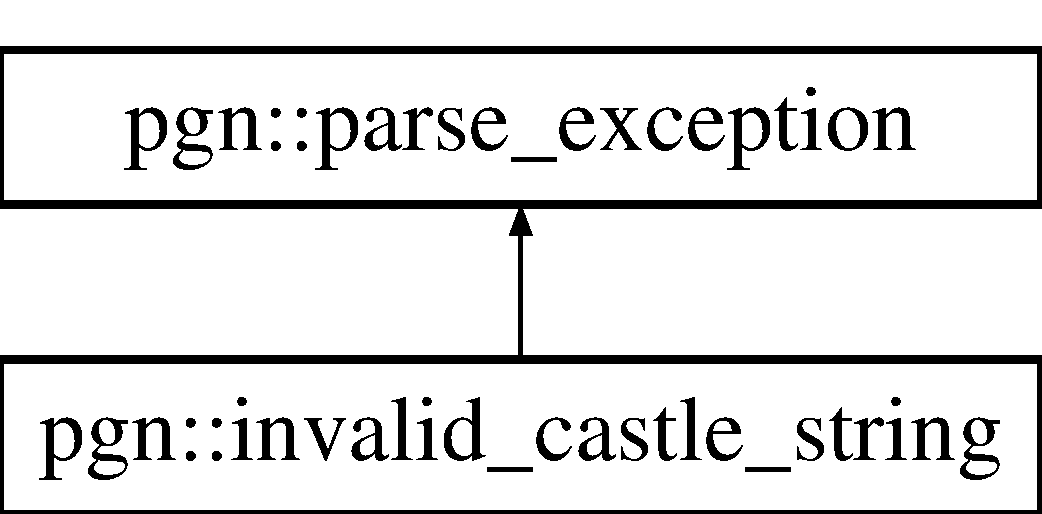
\includegraphics[height=2.000000cm]{classpgn_1_1invalid__castle__string}
\end{center}
\end{figure}


\subsection{Detailed Description}
Throws when castle in pgnfile is incorrect format. 

The documentation for this class was generated from the following file:\begin{DoxyCompactItemize}
\item 
src/libpgnm/src/PGNException.h\end{DoxyCompactItemize}

\hypertarget{classpgn_1_1invalid__ply__text}{
\section{pgn::invalid\_\-ply\_\-text Class Reference}
\label{classpgn_1_1invalid__ply__text}\index{pgn::invalid\_\-ply\_\-text@{pgn::invalid\_\-ply\_\-text}}
}


Throws when ply is in incorrect format.  




{\ttfamily \#include $<$PGNException.h$>$}

Inheritance diagram for pgn::invalid\_\-ply\_\-text:\begin{figure}[H]
\begin{center}
\leavevmode
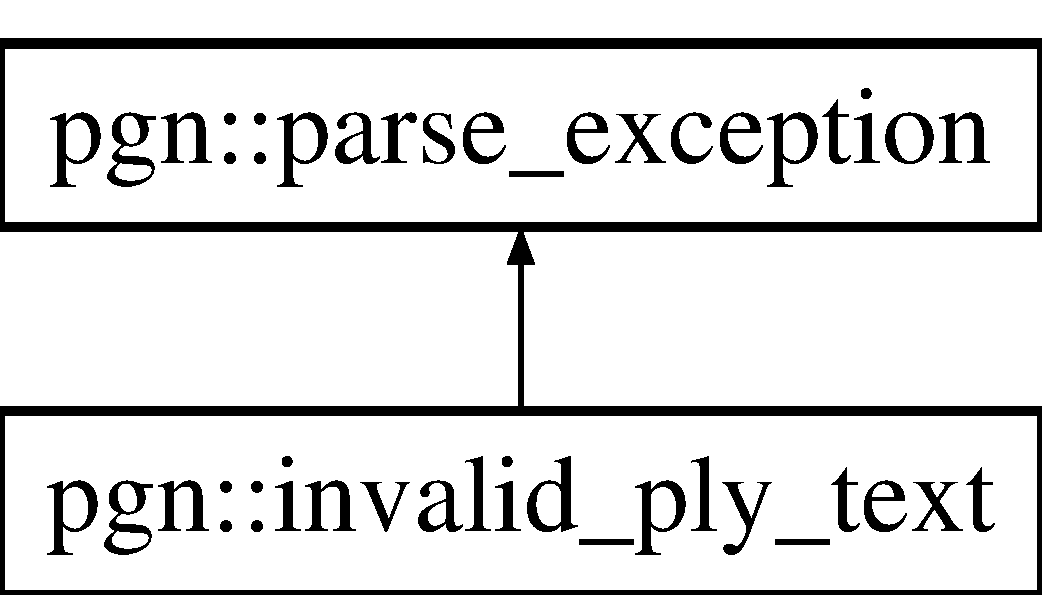
\includegraphics[height=2.000000cm]{classpgn_1_1invalid__ply__text}
\end{center}
\end{figure}
\subsection*{Public Member Functions}
\begin{DoxyCompactItemize}
\item 
\hypertarget{classpgn_1_1invalid__ply__text_ad345e8ac55e74e272c3a6f59611b7a94}{
{\bfseries invalid\_\-ply\_\-text} (const std::string \&ply)  throw ()}
\label{classpgn_1_1invalid__ply__text_ad345e8ac55e74e272c3a6f59611b7a94}

\end{DoxyCompactItemize}


\subsection{Detailed Description}
Throws when ply is in incorrect format. 

The documentation for this class was generated from the following file:\begin{DoxyCompactItemize}
\item 
src/libpgnm/src/PGNException.h\end{DoxyCompactItemize}

\hypertarget{classpgn_1_1invalid__result}{
\section{pgn::invalid\_\-result Class Reference}
\label{classpgn_1_1invalid__result}\index{pgn::invalid\_\-result@{pgn::invalid\_\-result}}
}


Throws when file contains result string in incorrect format.  




{\ttfamily \#include $<$PGNException.h$>$}

Inheritance diagram for pgn::invalid\_\-result:\begin{figure}[H]
\begin{center}
\leavevmode
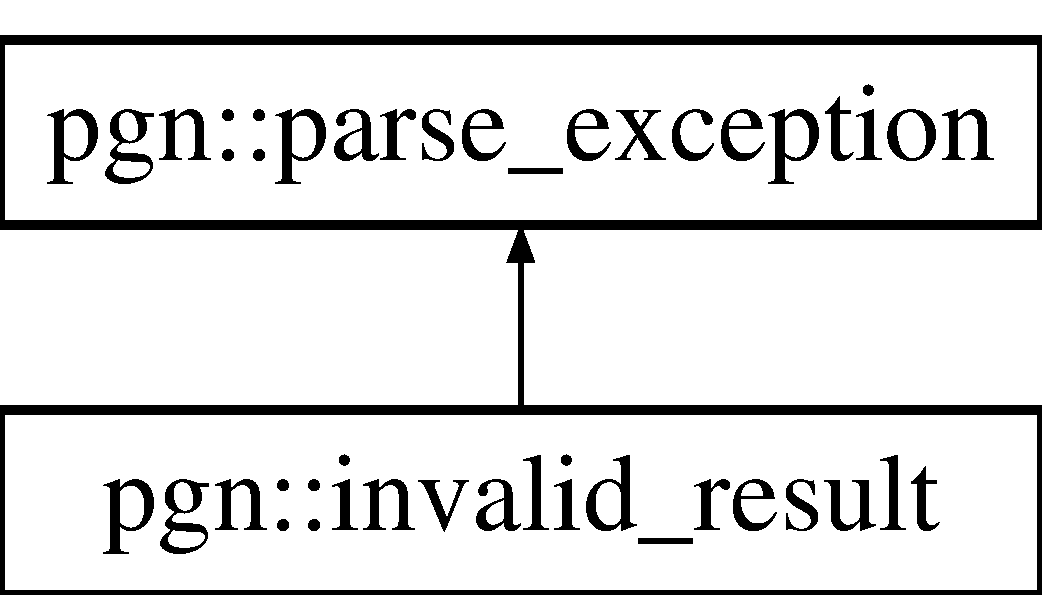
\includegraphics[height=2.000000cm]{classpgn_1_1invalid__result}
\end{center}
\end{figure}


\subsection{Detailed Description}
Throws when file contains result string in incorrect format. 

The documentation for this class was generated from the following file:\begin{DoxyCompactItemize}
\item 
src/libpgnm/src/PGNException.h\end{DoxyCompactItemize}

\hypertarget{classpgn_1_1invalid__tag}{
\section{pgn::invalid\_\-tag Class Reference}
\label{classpgn_1_1invalid__tag}\index{pgn::invalid\_\-tag@{pgn::invalid\_\-tag}}
}


Throws when file contains tag with wrong format.  




{\ttfamily \#include $<$PGNException.h$>$}

Inheritance diagram for pgn::invalid\_\-tag:\begin{figure}[H]
\begin{center}
\leavevmode
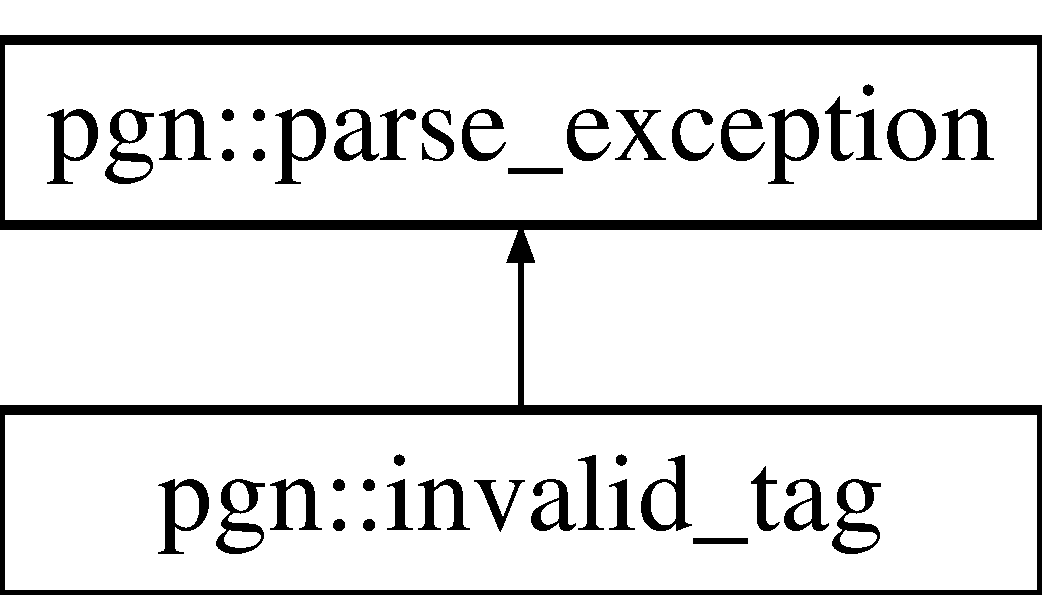
\includegraphics[height=2.000000cm]{classpgn_1_1invalid__tag}
\end{center}
\end{figure}


\subsection{Detailed Description}
Throws when file contains tag with wrong format. 

The documentation for this class was generated from the following file:\begin{DoxyCompactItemize}
\item 
src/libpgnm/src/PGNException.h\end{DoxyCompactItemize}

\hypertarget{classpgn_1_1MoveList_1_1iterator}{
\section{pgn::MoveList::iterator Class Reference}
\label{classpgn_1_1MoveList_1_1iterator}\index{pgn::MoveList::iterator@{pgn::MoveList::iterator}}
}
\subsection*{Public Member Functions}
\begin{DoxyCompactItemize}
\item 
\hypertarget{classpgn_1_1MoveList_1_1iterator_af578c8f6d3beb2b0c9069cb654d8a6f4}{
{\bfseries iterator} (const \hyperlink{classpgn_1_1MoveList}{MoveList} \&ml)}
\label{classpgn_1_1MoveList_1_1iterator_af578c8f6d3beb2b0c9069cb654d8a6f4}

\item 
\hypertarget{classpgn_1_1MoveList_1_1iterator_a008d340ba014f21eb7fbd3cf0a9f126a}{
{\bfseries iterator} (const \hyperlink{classpgn_1_1MoveList}{MoveList} \&ml, int)}
\label{classpgn_1_1MoveList_1_1iterator_a008d340ba014f21eb7fbd3cf0a9f126a}

\item 
\hypertarget{classpgn_1_1MoveList_1_1iterator_a6c58673ecca4aad9ad0db699cae876d4}{
{\bfseries iterator} (const \hyperlink{classpgn_1_1MoveList_1_1iterator}{iterator} \&)}
\label{classpgn_1_1MoveList_1_1iterator_a6c58673ecca4aad9ad0db699cae876d4}

\item 
\hypertarget{classpgn_1_1MoveList_1_1iterator_ac3a72a156b16bb58f0ee2decb1d02c21}{
\hyperlink{classpgn_1_1MoveList_1_1iterator}{iterator} \& {\bfseries operator=} (const \hyperlink{classpgn_1_1MoveList_1_1iterator}{iterator} \&)}
\label{classpgn_1_1MoveList_1_1iterator_ac3a72a156b16bb58f0ee2decb1d02c21}

\item 
\hypertarget{classpgn_1_1MoveList_1_1iterator_a6b64dc026f6549775782699a7e5aef14}{
\hyperlink{classpgn_1_1MoveList_1_1iterator}{iterator} \& {\bfseries operator++} ()}
\label{classpgn_1_1MoveList_1_1iterator_a6b64dc026f6549775782699a7e5aef14}

\item 
\hypertarget{classpgn_1_1MoveList_1_1iterator_a4397a978d4a01a4531155e0975bd294f}{
\hyperlink{classpgn_1_1MoveList_1_1iterator}{iterator} \& {\bfseries operator++} (int)}
\label{classpgn_1_1MoveList_1_1iterator_a4397a978d4a01a4531155e0975bd294f}

\item 
\hypertarget{classpgn_1_1MoveList_1_1iterator_a7c503b86c46a1eb18dd2cd0404d77369}{
\hyperlink{classpgn_1_1Move}{Move} $\ast$ {\bfseries operator-\/$>$} () const }
\label{classpgn_1_1MoveList_1_1iterator_a7c503b86c46a1eb18dd2cd0404d77369}

\item 
\hypertarget{classpgn_1_1MoveList_1_1iterator_a53bb952bf4b7855bab53b25ee0d1ea35}{
const \hyperlink{classpgn_1_1Move}{Move} \& {\bfseries operator$\ast$} () const }
\label{classpgn_1_1MoveList_1_1iterator_a53bb952bf4b7855bab53b25ee0d1ea35}

\item 
\hypertarget{classpgn_1_1MoveList_1_1iterator_a5bf2be372b1da555d6c16875005fa0bd}{
bool {\bfseries operator==} (const \hyperlink{classpgn_1_1MoveList_1_1iterator}{iterator} \&) const }
\label{classpgn_1_1MoveList_1_1iterator_a5bf2be372b1da555d6c16875005fa0bd}

\item 
\hypertarget{classpgn_1_1MoveList_1_1iterator_ac70080907e3d1c8869bf6ce035bcd6da}{
bool {\bfseries operator!=} (const \hyperlink{classpgn_1_1MoveList_1_1iterator}{iterator} \&) const }
\label{classpgn_1_1MoveList_1_1iterator_ac70080907e3d1c8869bf6ce035bcd6da}

\end{DoxyCompactItemize}


The documentation for this class was generated from the following file:\begin{DoxyCompactItemize}
\item 
src/libpgnm/src/PGNMoveList.h\end{DoxyCompactItemize}

\hypertarget{classpgn_1_1GameCollection_1_1iterator}{
\section{pgn::GameCollection::iterator Class Reference}
\label{classpgn_1_1GameCollection_1_1iterator}\index{pgn::GameCollection::iterator@{pgn::GameCollection::iterator}}
}


Instrument for safe iteration in \hyperlink{classpgn_1_1GameCollection}{pgn::GameCollection}.  




{\ttfamily \#include $<$PGNGameCollection.h$>$}

\subsection*{Public Member Functions}
\begin{DoxyCompactItemize}
\item 
\hypertarget{classpgn_1_1GameCollection_1_1iterator_a3b829c9fb4ca641aa3b972bff1a8e886}{
\hyperlink{classpgn_1_1GameCollection_1_1iterator_a3b829c9fb4ca641aa3b972bff1a8e886}{iterator} ()}
\label{classpgn_1_1GameCollection_1_1iterator_a3b829c9fb4ca641aa3b972bff1a8e886}

\begin{DoxyCompactList}\small\item\em Default constructor. \item\end{DoxyCompactList}\item 
\hyperlink{classpgn_1_1GameCollection_1_1iterator_a954bdfa9e2ea94b55bae8aae2f805887}{iterator} (const \hyperlink{classpgn_1_1GameCollection}{GameCollection} \&ml)
\begin{DoxyCompactList}\small\item\em Constructs iterator pointing to first game in given list. \item\end{DoxyCompactList}\item 
\hyperlink{classpgn_1_1GameCollection_1_1iterator_a41ba111b559fdfe85a970c98c8ed7093}{iterator} (const \hyperlink{classpgn_1_1GameCollection}{GameCollection} \&ml, int idx)
\begin{DoxyCompactList}\small\item\em Costructs iterator poinitng to game at idx. If at index idx is no game ml::end() will be returned. \item\end{DoxyCompactList}\item 
\hypertarget{classpgn_1_1GameCollection_1_1iterator_a4414c98751c5d952c8ae79ea46c44bcb}{
\hyperlink{classpgn_1_1GameCollection_1_1iterator_a4414c98751c5d952c8ae79ea46c44bcb}{iterator} (const \hyperlink{classpgn_1_1GameCollection_1_1iterator}{iterator} \&)}
\label{classpgn_1_1GameCollection_1_1iterator_a4414c98751c5d952c8ae79ea46c44bcb}

\begin{DoxyCompactList}\small\item\em Copy constructor. \item\end{DoxyCompactList}\item 
\hypertarget{classpgn_1_1GameCollection_1_1iterator_a6662899f24368d80f69645c4e3c417df}{
\hyperlink{classpgn_1_1GameCollection_1_1iterator_a6662899f24368d80f69645c4e3c417df}{$\sim$iterator} ()}
\label{classpgn_1_1GameCollection_1_1iterator_a6662899f24368d80f69645c4e3c417df}

\begin{DoxyCompactList}\small\item\em Destructor. \item\end{DoxyCompactList}\item 
\hyperlink{classpgn_1_1GameCollection_1_1iterator}{iterator} \& \hyperlink{classpgn_1_1GameCollection_1_1iterator_af2b22a067e26861e9616d43cd6deea39}{operator=} (const \hyperlink{classpgn_1_1GameCollection_1_1iterator}{iterator} \&src)
\begin{DoxyCompactList}\small\item\em Sets current iterator pointing as given. \item\end{DoxyCompactList}\item 
\hypertarget{classpgn_1_1GameCollection_1_1iterator_af5677cb98e09007563f052b7b01bb14d}{
\hyperlink{classpgn_1_1GameCollection_1_1iterator}{iterator} \& \hyperlink{classpgn_1_1GameCollection_1_1iterator_af5677cb98e09007563f052b7b01bb14d}{operator++} ()}
\label{classpgn_1_1GameCollection_1_1iterator_af5677cb98e09007563f052b7b01bb14d}

\begin{DoxyCompactList}\small\item\em Sets iterator point to next game. \item\end{DoxyCompactList}\item 
\hyperlink{classpgn_1_1GameCollection_1_1iterator}{iterator} \& \hyperlink{classpgn_1_1GameCollection_1_1iterator_ab728b4cdfc18844ee564b74443b09bdf}{operator++} (int i)
\begin{DoxyCompactList}\small\item\em Moves iterator to {\itshape  positions forward. \/}\item\end{DoxyCompactList}\item 
\hyperlink{classpgn_1_1Game}{Game} $\ast$ \hyperlink{classpgn_1_1GameCollection_1_1iterator_a245601d25335e1ba67874d3d70382bb0}{operator-\/$>$} () const 
\begin{DoxyCompactList}\small\item\em Get game iterator is pointing to. \item\end{DoxyCompactList}\item 
const \hyperlink{classpgn_1_1Game}{Game} \& \hyperlink{classpgn_1_1GameCollection_1_1iterator_ae1c72b3ca9c338ccc117315f7551eea2}{operator$\ast$} () const 
\begin{DoxyCompactList}\small\item\em Get game iterator is pointing to. \item\end{DoxyCompactList}\item 
bool \hyperlink{classpgn_1_1GameCollection_1_1iterator_ad5b3ab7c17b8bcd6dcc1122256abda56}{operator==} (const \hyperlink{classpgn_1_1GameCollection_1_1iterator}{iterator} \&) const 
\begin{DoxyCompactList}\small\item\em Checks are two iterator pointing to same game. \item\end{DoxyCompactList}\item 
\hypertarget{classpgn_1_1GameCollection_1_1iterator_ab93ed70b78aa6461dc5ea515a3a0592e}{
bool \hyperlink{classpgn_1_1GameCollection_1_1iterator_ab93ed70b78aa6461dc5ea515a3a0592e}{operator!=} (const \hyperlink{classpgn_1_1GameCollection_1_1iterator}{iterator} \&) const }
\label{classpgn_1_1GameCollection_1_1iterator_ab93ed70b78aa6461dc5ea515a3a0592e}

\begin{DoxyCompactList}\small\item\em Negative variant of operator==. \item\end{DoxyCompactList}\end{DoxyCompactItemize}


\subsection{Detailed Description}
Instrument for safe iteration in \hyperlink{classpgn_1_1GameCollection}{pgn::GameCollection}. 

\subsection{Constructor \& Destructor Documentation}
\hypertarget{classpgn_1_1GameCollection_1_1iterator_a954bdfa9e2ea94b55bae8aae2f805887}{
\index{pgn::GameCollection::iterator@{pgn::GameCollection::iterator}!iterator@{iterator}}
\index{iterator@{iterator}!pgn::GameCollection::iterator@{pgn::GameCollection::iterator}}
\subsubsection[{iterator}]{\setlength{\rightskip}{0pt plus 5cm}pgn::GameCollection::iterator::iterator (
\begin{DoxyParamCaption}
\item[{const {\bf GameCollection} \&}]{ml}
\end{DoxyParamCaption}
)}}
\label{classpgn_1_1GameCollection_1_1iterator_a954bdfa9e2ea94b55bae8aae2f805887}


Constructs iterator pointing to first game in given list. 


\begin{DoxyParams}{Parameters}
{\em ml} & Collection to iteration. \\
\hline
\end{DoxyParams}
\hypertarget{classpgn_1_1GameCollection_1_1iterator_a41ba111b559fdfe85a970c98c8ed7093}{
\index{pgn::GameCollection::iterator@{pgn::GameCollection::iterator}!iterator@{iterator}}
\index{iterator@{iterator}!pgn::GameCollection::iterator@{pgn::GameCollection::iterator}}
\subsubsection[{iterator}]{\setlength{\rightskip}{0pt plus 5cm}pgn::GameCollection::iterator::iterator (
\begin{DoxyParamCaption}
\item[{const {\bf GameCollection} \&}]{ml, }
\item[{int}]{idx}
\end{DoxyParamCaption}
)}}
\label{classpgn_1_1GameCollection_1_1iterator_a41ba111b559fdfe85a970c98c8ed7093}


Costructs iterator poinitng to game at idx. If at index idx is no game ml::end() will be returned. 


\begin{DoxyParams}{Parameters}
{\em ml} & Collection to iteration. \\
\hline
{\em idx} & Iterator position. \\
\hline
\end{DoxyParams}


\subsection{Member Function Documentation}
\hypertarget{classpgn_1_1GameCollection_1_1iterator_ae1c72b3ca9c338ccc117315f7551eea2}{
\index{pgn::GameCollection::iterator@{pgn::GameCollection::iterator}!operator$\ast$@{operator$\ast$}}
\index{operator$\ast$@{operator$\ast$}!pgn::GameCollection::iterator@{pgn::GameCollection::iterator}}
\subsubsection[{operator$\ast$}]{\setlength{\rightskip}{0pt plus 5cm}const {\bf Game}\& pgn::GameCollection::iterator::operator$\ast$ (
\begin{DoxyParamCaption}
{}
\end{DoxyParamCaption}
) const}}
\label{classpgn_1_1GameCollection_1_1iterator_ae1c72b3ca9c338ccc117315f7551eea2}


Get game iterator is pointing to. 

\begin{DoxyReturn}{Returns}
\hyperlink{classpgn_1_1Game}{Game} iterator is pointing to. 
\end{DoxyReturn}
\hypertarget{classpgn_1_1GameCollection_1_1iterator_ab728b4cdfc18844ee564b74443b09bdf}{
\index{pgn::GameCollection::iterator@{pgn::GameCollection::iterator}!operator++@{operator++}}
\index{operator++@{operator++}!pgn::GameCollection::iterator@{pgn::GameCollection::iterator}}
\subsubsection[{operator++}]{\setlength{\rightskip}{0pt plus 5cm}{\bf iterator}\& pgn::GameCollection::iterator::operator++ (
\begin{DoxyParamCaption}
\item[{int}]{i}
\end{DoxyParamCaption}
)}}
\label{classpgn_1_1GameCollection_1_1iterator_ab728b4cdfc18844ee564b74443b09bdf}


Moves iterator to {\itshape  positions forward. \/}


\begin{DoxyParams}{Parameters}
{\em i} & Positions count to be forwarded. \\
\hline
\end{DoxyParams}
\hypertarget{classpgn_1_1GameCollection_1_1iterator_a245601d25335e1ba67874d3d70382bb0}{
\index{pgn::GameCollection::iterator@{pgn::GameCollection::iterator}!operator-\/$>$@{operator-\/$>$}}
\index{operator-\/$>$@{operator-\/$>$}!pgn::GameCollection::iterator@{pgn::GameCollection::iterator}}
\subsubsection[{operator-\/$>$}]{\setlength{\rightskip}{0pt plus 5cm}{\bf Game}$\ast$ pgn::GameCollection::iterator::operator-\/$>$ (
\begin{DoxyParamCaption}
{}
\end{DoxyParamCaption}
) const}}
\label{classpgn_1_1GameCollection_1_1iterator_a245601d25335e1ba67874d3d70382bb0}


Get game iterator is pointing to. 

\begin{DoxyReturn}{Returns}
\hyperlink{classpgn_1_1Game}{Game} iterator is pointing to. 
\end{DoxyReturn}
\hypertarget{classpgn_1_1GameCollection_1_1iterator_af2b22a067e26861e9616d43cd6deea39}{
\index{pgn::GameCollection::iterator@{pgn::GameCollection::iterator}!operator=@{operator=}}
\index{operator=@{operator=}!pgn::GameCollection::iterator@{pgn::GameCollection::iterator}}
\subsubsection[{operator=}]{\setlength{\rightskip}{0pt plus 5cm}{\bf iterator}\& pgn::GameCollection::iterator::operator= (
\begin{DoxyParamCaption}
\item[{const {\bf iterator} \&}]{src}
\end{DoxyParamCaption}
)}}
\label{classpgn_1_1GameCollection_1_1iterator_af2b22a067e26861e9616d43cd6deea39}


Sets current iterator pointing as given. 


\begin{DoxyParams}{Parameters}
{\em src} & Source iterator. \\
\hline
\end{DoxyParams}
\hypertarget{classpgn_1_1GameCollection_1_1iterator_ad5b3ab7c17b8bcd6dcc1122256abda56}{
\index{pgn::GameCollection::iterator@{pgn::GameCollection::iterator}!operator==@{operator==}}
\index{operator==@{operator==}!pgn::GameCollection::iterator@{pgn::GameCollection::iterator}}
\subsubsection[{operator==}]{\setlength{\rightskip}{0pt plus 5cm}bool pgn::GameCollection::iterator::operator== (
\begin{DoxyParamCaption}
\item[{const {\bf iterator} \&}]{}
\end{DoxyParamCaption}
) const}}
\label{classpgn_1_1GameCollection_1_1iterator_ad5b3ab7c17b8bcd6dcc1122256abda56}


Checks are two iterator pointing to same game. 

\begin{DoxyReturn}{Returns}
true if iterators are equal. 
\end{DoxyReturn}


The documentation for this class was generated from the following file:\begin{DoxyCompactItemize}
\item 
src/libpgnm/src/PGNGameCollection.h\end{DoxyCompactItemize}

\hypertarget{classpgn_1_1TagList_1_1iterator}{
\section{pgn::TagList::iterator Class Reference}
\label{classpgn_1_1TagList_1_1iterator}\index{pgn::TagList::iterator@{pgn::TagList::iterator}}
}
\subsection*{Public Member Functions}
\begin{DoxyCompactItemize}
\item 
\hypertarget{classpgn_1_1TagList_1_1iterator_a01f4186540355b25789385a9b3589021}{
{\bfseries iterator} (const \hyperlink{classpgn_1_1TagList}{TagList} \&tl)}
\label{classpgn_1_1TagList_1_1iterator_a01f4186540355b25789385a9b3589021}

\item 
\hypertarget{classpgn_1_1TagList_1_1iterator_a338f14cfdab089e4c4ec62b417d13ff9}{
{\bfseries iterator} (const \hyperlink{classpgn_1_1TagList}{TagList} \&tl, int)}
\label{classpgn_1_1TagList_1_1iterator_a338f14cfdab089e4c4ec62b417d13ff9}

\item 
\hypertarget{classpgn_1_1TagList_1_1iterator_a5e4bd608535b51f119d338b6eecc603d}{
{\bfseries iterator} (const \hyperlink{classpgn_1_1TagList_1_1iterator}{iterator} \&)}
\label{classpgn_1_1TagList_1_1iterator_a5e4bd608535b51f119d338b6eecc603d}

\item 
\hypertarget{classpgn_1_1TagList_1_1iterator_ad12529a9935ddda19be039e870b9093d}{
\hyperlink{classpgn_1_1TagList_1_1iterator}{iterator} \& {\bfseries operator=} (const \hyperlink{classpgn_1_1TagList_1_1iterator}{iterator} \&)}
\label{classpgn_1_1TagList_1_1iterator_ad12529a9935ddda19be039e870b9093d}

\item 
\hypertarget{classpgn_1_1TagList_1_1iterator_a2671cbe94f0cfc8d377acfa21a8d378f}{
\hyperlink{classpgn_1_1TagList_1_1iterator}{iterator} \& {\bfseries operator++} ()}
\label{classpgn_1_1TagList_1_1iterator_a2671cbe94f0cfc8d377acfa21a8d378f}

\item 
\hypertarget{classpgn_1_1TagList_1_1iterator_a8611f33610533dde89fcefeb630902b5}{
\hyperlink{classpgn_1_1TagList_1_1iterator}{iterator} \& {\bfseries operator++} (int)}
\label{classpgn_1_1TagList_1_1iterator_a8611f33610533dde89fcefeb630902b5}

\item 
\hypertarget{classpgn_1_1TagList_1_1iterator_a3498a4bf6bf90f673da05387db181921}{
\hyperlink{classpgn_1_1Tag}{Tag} $\ast$ {\bfseries operator-\/$>$} () const }
\label{classpgn_1_1TagList_1_1iterator_a3498a4bf6bf90f673da05387db181921}

\item 
\hypertarget{classpgn_1_1TagList_1_1iterator_afc167531276b3f8ad75efd7484169596}{
const \hyperlink{classpgn_1_1Tag}{Tag} \& {\bfseries operator$\ast$} () const }
\label{classpgn_1_1TagList_1_1iterator_afc167531276b3f8ad75efd7484169596}

\item 
\hypertarget{classpgn_1_1TagList_1_1iterator_ab569fc7d7d24af664bb0e533264c9342}{
bool {\bfseries operator==} (const \hyperlink{classpgn_1_1TagList_1_1iterator}{iterator} \&) const }
\label{classpgn_1_1TagList_1_1iterator_ab569fc7d7d24af664bb0e533264c9342}

\item 
\hypertarget{classpgn_1_1TagList_1_1iterator_a1c62ef962f35a95d4b2045413e949842}{
bool {\bfseries operator!=} (const \hyperlink{classpgn_1_1TagList_1_1iterator}{iterator} \&) const }
\label{classpgn_1_1TagList_1_1iterator_a1c62ef962f35a95d4b2045413e949842}

\end{DoxyCompactItemize}


The documentation for this class was generated from the following file:\begin{DoxyCompactItemize}
\item 
src/libpgnm/src/PGNTagList.h\end{DoxyCompactItemize}

\hypertarget{classpgn_1_1missing__result}{
\section{pgn::missing\_\-result Class Reference}
\label{classpgn_1_1missing__result}\index{pgn::missing\_\-result@{pgn::missing\_\-result}}
}


Throws when game/file does not contain information about game result.  




{\ttfamily \#include $<$PGNException.h$>$}

Inheritance diagram for pgn::missing\_\-result:\begin{figure}[H]
\begin{center}
\leavevmode
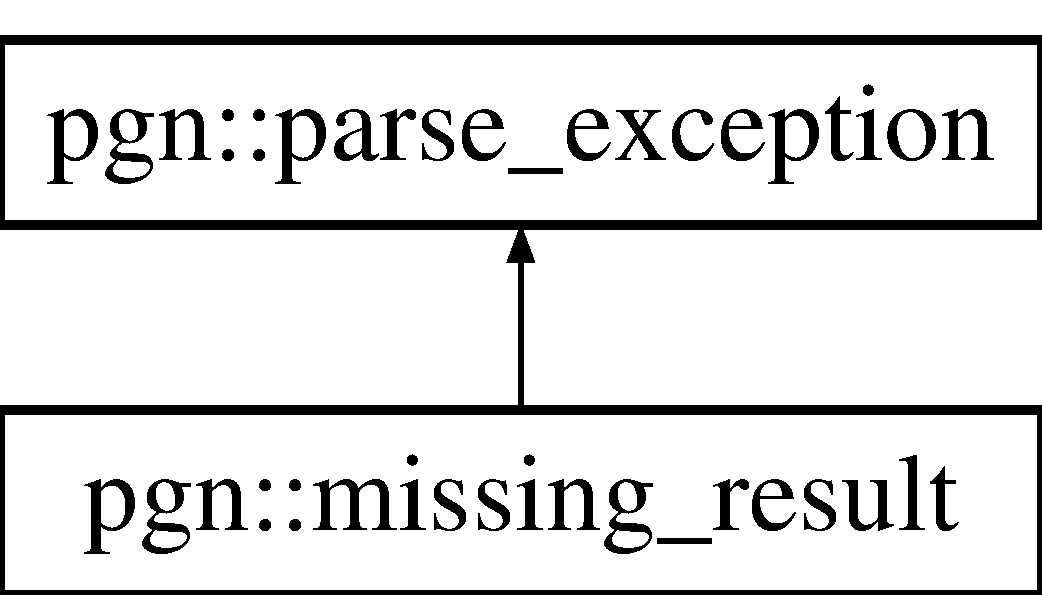
\includegraphics[height=2.000000cm]{classpgn_1_1missing__result}
\end{center}
\end{figure}


\subsection{Detailed Description}
Throws when game/file does not contain information about game result. 

The documentation for this class was generated from the following file:\begin{DoxyCompactItemize}
\item 
src/libpgnm/src/PGNException.h\end{DoxyCompactItemize}

\hypertarget{classpgn_1_1Move}{
\section{pgn::Move Class Reference}
\label{classpgn_1_1Move}\index{pgn::Move@{pgn::Move}}
}
\subsection*{Public Member Functions}
\begin{DoxyCompactItemize}
\item 
\hypertarget{classpgn_1_1Move_a28247b92783975d25036b9d5194114b4}{
{\bfseries Move} (const \hyperlink{classpgn_1_1Move}{Move} \&src)}
\label{classpgn_1_1Move_a28247b92783975d25036b9d5194114b4}

\item 
\hypertarget{classpgn_1_1Move_a25045059decc1f06eb0088f52c277ea3}{
{\bfseries Move} (const \hyperlink{classpgn_1_1Ply}{Ply} $\ast$white, const \hyperlink{classpgn_1_1Ply}{Ply} $\ast$black, int number)}
\label{classpgn_1_1Move_a25045059decc1f06eb0088f52c277ea3}

\item 
\hypertarget{classpgn_1_1Move_a13eaa8cab0874d6f5c30017c179ca608}{
\hyperlink{classpgn_1_1Move}{Move} \& {\bfseries operator=} (const \hyperlink{classpgn_1_1Move}{Move} \&src)}
\label{classpgn_1_1Move_a13eaa8cab0874d6f5c30017c179ca608}

\item 
\hypertarget{classpgn_1_1Move_ab29d7ad0a246c58f53840c30163ff932}{
bool {\bfseries operator==} (const \hyperlink{classpgn_1_1Move}{Move} \&src) const }
\label{classpgn_1_1Move_ab29d7ad0a246c58f53840c30163ff932}

\item 
\hypertarget{classpgn_1_1Move_a59795e9c42731f979271d86546c254aa}{
bool {\bfseries operator!=} (const \hyperlink{classpgn_1_1Move}{Move} \&src) const }
\label{classpgn_1_1Move_a59795e9c42731f979271d86546c254aa}

\item 
\hypertarget{classpgn_1_1Move_ad15aa895b133bf43304b147bc3db9e5d}{
bool {\bfseries isCheckMate} () const }
\label{classpgn_1_1Move_ad15aa895b133bf43304b147bc3db9e5d}

\item 
\hypertarget{classpgn_1_1Move_a0321dd73f271684cf7040bb61c1934e3}{
\hyperlink{classpgn_1_1Ply}{Ply} $\ast$ {\bfseries white} () const }
\label{classpgn_1_1Move_a0321dd73f271684cf7040bb61c1934e3}

\item 
\hypertarget{classpgn_1_1Move_a112464932b1bf070ef1c465fadb9c4b1}{
\hyperlink{classpgn_1_1Ply}{Ply} $\ast$ {\bfseries black} () const }
\label{classpgn_1_1Move_a112464932b1bf070ef1c465fadb9c4b1}

\item 
\hypertarget{classpgn_1_1Move_a0f09e103caca4e9484779d67e4ff2e54}{
std::string {\bfseries toStdString} ()}
\label{classpgn_1_1Move_a0f09e103caca4e9484779d67e4ff2e54}

\end{DoxyCompactItemize}
\subsection*{Static Public Member Functions}
\begin{DoxyCompactItemize}
\item 
\hypertarget{classpgn_1_1Move_ab69fb9cbd8ad8107e6d6264a66cf74af}{
static std::string {\bfseries itoa} (int n)}
\label{classpgn_1_1Move_ab69fb9cbd8ad8107e6d6264a66cf74af}

\end{DoxyCompactItemize}
\subsection*{Friends}
\begin{DoxyCompactItemize}
\item 
\hypertarget{classpgn_1_1Move_a59221be82ec792c0a15addf8746a667c}{
std::ostream \& {\bfseries operator$<$$<$} (std::ostream \&os, const \hyperlink{classpgn_1_1Move}{Move} \&src)}
\label{classpgn_1_1Move_a59221be82ec792c0a15addf8746a667c}

\end{DoxyCompactItemize}


The documentation for this class was generated from the following file:\begin{DoxyCompactItemize}
\item 
src/libpgnm/src/PGNMove.h\end{DoxyCompactItemize}

\hypertarget{classpgn_1_1MoveList}{
\section{pgn::MoveList Class Reference}
\label{classpgn_1_1MoveList}\index{pgn::MoveList@{pgn::MoveList}}
}
\subsection*{Classes}
\begin{DoxyCompactItemize}
\item 
class \hyperlink{classpgn_1_1MoveList_1_1iterator}{iterator}
\end{DoxyCompactItemize}
\subsection*{Public Member Functions}
\begin{DoxyCompactItemize}
\item 
\hypertarget{classpgn_1_1MoveList_acc752e85d5cf6c1c99981ec4d12ea15c}{
{\bfseries MoveList} (const \hyperlink{classpgn_1_1MoveList}{MoveList} \&src)}
\label{classpgn_1_1MoveList_acc752e85d5cf6c1c99981ec4d12ea15c}

\item 
\hypertarget{classpgn_1_1MoveList_abb501f7f61d89873a9b0de5a7e88325c}{
\hyperlink{classpgn_1_1MoveList}{MoveList} \& {\bfseries operator=} (const \hyperlink{classpgn_1_1MoveList}{MoveList} \&src)}
\label{classpgn_1_1MoveList_abb501f7f61d89873a9b0de5a7e88325c}

\item 
\hypertarget{classpgn_1_1MoveList_a0658540f6cfae1ce91f452727619b86a}{
bool {\bfseries operator==} (const \hyperlink{classpgn_1_1MoveList}{MoveList} \&src) const }
\label{classpgn_1_1MoveList_a0658540f6cfae1ce91f452727619b86a}

\item 
\hypertarget{classpgn_1_1MoveList_a1202bbbcd297b01dbda1b553986a2ded}{
bool {\bfseries operator!=} (const \hyperlink{classpgn_1_1MoveList}{MoveList} \&src) const }
\label{classpgn_1_1MoveList_a1202bbbcd297b01dbda1b553986a2ded}

\item 
\hypertarget{classpgn_1_1MoveList_a3b4ce80ae6b3c3a3420188a35b80a7cb}{
\hyperlink{classpgn_1_1Move}{Move} {\bfseries operator\mbox{[}$\,$\mbox{]}} (int idx)}
\label{classpgn_1_1MoveList_a3b4ce80ae6b3c3a3420188a35b80a7cb}

\item 
\hypertarget{classpgn_1_1MoveList_adf332a57924c82ae7cfc72667e071f4c}{
void {\bfseries insert} (const \hyperlink{classpgn_1_1Move}{Move} \&src)}
\label{classpgn_1_1MoveList_adf332a57924c82ae7cfc72667e071f4c}

\item 
\hypertarget{classpgn_1_1MoveList_a3ddb137e4ca42acfb38b8dd0799a973a}{
bool {\bfseries find} (const \hyperlink{classpgn_1_1Move}{Move} \&src) const }
\label{classpgn_1_1MoveList_a3ddb137e4ca42acfb38b8dd0799a973a}

\item 
\hypertarget{classpgn_1_1MoveList_addc4ac0affa66c4b949b51ca5b78c55f}{
int {\bfseries size} () const }
\label{classpgn_1_1MoveList_addc4ac0affa66c4b949b51ca5b78c55f}

\item 
\hypertarget{classpgn_1_1MoveList_a73b42c6cbd8f7e226834ab0c9ee34f09}{
\hyperlink{classpgn_1_1MoveList_1_1iterator}{iterator} {\bfseries begin} () const }
\label{classpgn_1_1MoveList_a73b42c6cbd8f7e226834ab0c9ee34f09}

\item 
\hypertarget{classpgn_1_1MoveList_a14a21251ba1a08e8934ec204c9558c82}{
\hyperlink{classpgn_1_1MoveList_1_1iterator}{iterator} {\bfseries end} () const }
\label{classpgn_1_1MoveList_a14a21251ba1a08e8934ec204c9558c82}

\item 
\hypertarget{classpgn_1_1MoveList_a97c94457913b294e15d492dd2a2e8c19}{
std::string {\bfseries toStdString} ()}
\label{classpgn_1_1MoveList_a97c94457913b294e15d492dd2a2e8c19}

\end{DoxyCompactItemize}
\subsection*{Friends}
\begin{DoxyCompactItemize}
\item 
\hypertarget{classpgn_1_1MoveList_a67171474c4da6cc8efe0c7fafefd2b2d}{
class {\bfseries iterator}}
\label{classpgn_1_1MoveList_a67171474c4da6cc8efe0c7fafefd2b2d}

\item 
\hypertarget{classpgn_1_1MoveList_a0d05100a7283d96193fddbfc7624fc9c}{
std::ostream \& {\bfseries operator$<$$<$} (std::ostream \&os, const \hyperlink{classpgn_1_1MoveList}{MoveList} \&src)}
\label{classpgn_1_1MoveList_a0d05100a7283d96193fddbfc7624fc9c}

\end{DoxyCompactItemize}


The documentation for this class was generated from the following file:\begin{DoxyCompactItemize}
\item 
src/libpgnm/src/PGNMoveList.h\end{DoxyCompactItemize}

\hypertarget{classpgn_1_1parse__exception}{
\section{pgn::parse\_\-exception Class Reference}
\label{classpgn_1_1parse__exception}\index{pgn::parse\_\-exception@{pgn::parse\_\-exception}}
}


Represents exceptions which must be throwed on parsing.  




{\ttfamily \#include $<$PGNException.h$>$}

Inheritance diagram for pgn::parse\_\-exception:\begin{figure}[H]
\begin{center}
\leavevmode
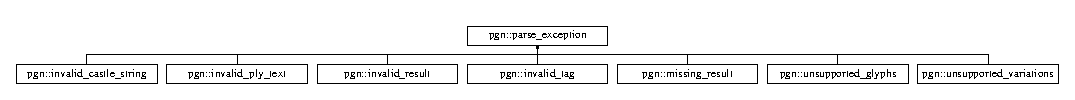
\includegraphics[height=0.893855cm]{classpgn_1_1parse__exception}
\end{center}
\end{figure}
\subsection*{Public Member Functions}
\begin{DoxyCompactItemize}
\item 
\hyperlink{classpgn_1_1parse__exception_a7bae04deaf606dd6988cfefa933b7101}{parse\_\-exception} (const std::string \&message)  throw ()
\begin{DoxyCompactList}\small\item\em Represents parse exception with given message. \item\end{DoxyCompactList}\item 
void \hyperlink{classpgn_1_1parse__exception_aaf1aa4e8c2a2eaf549ba766b94b13fb2}{bindParsingText} (const std::string \&parsingtext)  throw ()
\begin{DoxyCompactList}\small\item\em Sets text which is wrong. \item\end{DoxyCompactList}\item 
const char $\ast$ \hyperlink{classpgn_1_1parse__exception_abfdb03d89f8b9f5460cbdc83c82f177a}{parsing\_\-text} () const   throw ()
\begin{DoxyCompactList}\small\item\em Gets text which is wrong. \item\end{DoxyCompactList}\item 
virtual const char $\ast$ \hyperlink{classpgn_1_1parse__exception_a6b9a11cd8e08364f76d073891407ea41}{what} () const   throw ()
\begin{DoxyCompactList}\small\item\em Gets additional information about exception. \item\end{DoxyCompactList}\end{DoxyCompactItemize}


\subsection{Detailed Description}
Represents exceptions which must be throwed on parsing. 

\subsection{Constructor \& Destructor Documentation}
\hypertarget{classpgn_1_1parse__exception_a7bae04deaf606dd6988cfefa933b7101}{
\index{pgn::parse\_\-exception@{pgn::parse\_\-exception}!parse\_\-exception@{parse\_\-exception}}
\index{parse\_\-exception@{parse\_\-exception}!pgn::parse_exception@{pgn::parse\_\-exception}}
\subsubsection[{parse\_\-exception}]{\setlength{\rightskip}{0pt plus 5cm}pgn::parse\_\-exception::parse\_\-exception (
\begin{DoxyParamCaption}
\item[{const std::string \&}]{message}
\end{DoxyParamCaption}
)  throw ()\hspace{0.3cm}{\ttfamily  \mbox{[}inline\mbox{]}}}}
\label{classpgn_1_1parse__exception_a7bae04deaf606dd6988cfefa933b7101}


Represents parse exception with given message. 


\begin{DoxyParams}{Parameters}
{\em message} & Text message, description of error. \\
\hline
\end{DoxyParams}


\subsection{Member Function Documentation}
\hypertarget{classpgn_1_1parse__exception_aaf1aa4e8c2a2eaf549ba766b94b13fb2}{
\index{pgn::parse\_\-exception@{pgn::parse\_\-exception}!bindParsingText@{bindParsingText}}
\index{bindParsingText@{bindParsingText}!pgn::parse_exception@{pgn::parse\_\-exception}}
\subsubsection[{bindParsingText}]{\setlength{\rightskip}{0pt plus 5cm}void pgn::parse\_\-exception::bindParsingText (
\begin{DoxyParamCaption}
\item[{const std::string \&}]{parsingtext}
\end{DoxyParamCaption}
)  throw ()\hspace{0.3cm}{\ttfamily  \mbox{[}inline\mbox{]}}}}
\label{classpgn_1_1parse__exception_aaf1aa4e8c2a2eaf549ba766b94b13fb2}


Sets text which is wrong. 


\begin{DoxyParams}{Parameters}
{\em parsingtext} & Wrong text from PGN file. \\
\hline
\end{DoxyParams}
\hypertarget{classpgn_1_1parse__exception_abfdb03d89f8b9f5460cbdc83c82f177a}{
\index{pgn::parse\_\-exception@{pgn::parse\_\-exception}!parsing\_\-text@{parsing\_\-text}}
\index{parsing\_\-text@{parsing\_\-text}!pgn::parse_exception@{pgn::parse\_\-exception}}
\subsubsection[{parsing\_\-text}]{\setlength{\rightskip}{0pt plus 5cm}const char$\ast$ pgn::parse\_\-exception::parsing\_\-text (
\begin{DoxyParamCaption}
{}
\end{DoxyParamCaption}
) const  throw ()\hspace{0.3cm}{\ttfamily  \mbox{[}inline\mbox{]}}}}
\label{classpgn_1_1parse__exception_abfdb03d89f8b9f5460cbdc83c82f177a}


Gets text which is wrong. 

\begin{DoxyReturn}{Returns}
Wrong text fomr PGN file. 
\end{DoxyReturn}
\hypertarget{classpgn_1_1parse__exception_a6b9a11cd8e08364f76d073891407ea41}{
\index{pgn::parse\_\-exception@{pgn::parse\_\-exception}!what@{what}}
\index{what@{what}!pgn::parse_exception@{pgn::parse\_\-exception}}
\subsubsection[{what}]{\setlength{\rightskip}{0pt plus 5cm}virtual const char$\ast$ pgn::parse\_\-exception::what (
\begin{DoxyParamCaption}
{}
\end{DoxyParamCaption}
) const  throw ()\hspace{0.3cm}{\ttfamily  \mbox{[}inline, virtual\mbox{]}}}}
\label{classpgn_1_1parse__exception_a6b9a11cd8e08364f76d073891407ea41}


Gets additional information about exception. 

\begin{DoxyReturn}{Returns}
Additional information. 
\end{DoxyReturn}


The documentation for this class was generated from the following file:\begin{DoxyCompactItemize}
\item 
src/libpgnm/src/PGNException.h\end{DoxyCompactItemize}

\hypertarget{classpgn_1_1Parser}{
\section{pgn::Parser Class Reference}
\label{classpgn_1_1Parser}\index{pgn::Parser@{pgn::Parser}}
}
\subsection*{Public Member Functions}
\begin{DoxyCompactItemize}
\item 
\hypertarget{classpgn_1_1Parser_a9feaee2ae6fc57fdfa7de8e405291082}{
bool {\bfseries getGameCollection} (std::string::const\_\-iterator \&itr1, const std::string::const\_\-iterator \&itr2, \hyperlink{classpgn_1_1GameCollection}{pgn::GameCollection} \&out)}
\label{classpgn_1_1Parser_a9feaee2ae6fc57fdfa7de8e405291082}

\item 
\hypertarget{classpgn_1_1Parser_a75fb06094fc412eb3197cda813ec7e5e}{
\hyperlink{classpgn_1_1Game}{pgn::Game} $\ast$ {\bfseries getGame} (std::string::const\_\-iterator \&itr1, const std::string::const\_\-iterator \&itr2)}
\label{classpgn_1_1Parser_a75fb06094fc412eb3197cda813ec7e5e}

\item 
\hypertarget{classpgn_1_1Parser_afbb1aee64b477bafca8ab2486b3e669f}{
bool {\bfseries getMoveList} (std::string::const\_\-iterator \&itr1, const std::string::const\_\-iterator \&itr2, \hyperlink{classpgn_1_1MoveList}{pgn::MoveList} \&out)}
\label{classpgn_1_1Parser_afbb1aee64b477bafca8ab2486b3e669f}

\item 
\hypertarget{classpgn_1_1Parser_a38ccb9809b26c90cebe525e342ffd6cc}{
\hyperlink{classpgn_1_1Move}{pgn::Move} $\ast$ {\bfseries getMove} (std::string::const\_\-iterator \&itr1, const std::string::const\_\-iterator \&itr2)}
\label{classpgn_1_1Parser_a38ccb9809b26c90cebe525e342ffd6cc}

\item 
\hypertarget{classpgn_1_1Parser_a4efc9cafd449f453b498691625137acd}{
\hyperlink{classpgn_1_1Ply}{pgn::Ply} $\ast$ {\bfseries getPly} (std::string::const\_\-iterator \&itr1, const std::string::const\_\-iterator \&itr2)}
\label{classpgn_1_1Parser_a4efc9cafd449f453b498691625137acd}

\item 
\hypertarget{classpgn_1_1Parser_aa75b1285609ed972cf7032b4c89d5a04}{
bool {\bfseries getTagList} (std::string::const\_\-iterator \&itr1, const std::string::const\_\-iterator \&itr2, \hyperlink{classpgn_1_1TagList}{pgn::TagList} \&out)}
\label{classpgn_1_1Parser_aa75b1285609ed972cf7032b4c89d5a04}

\item 
\hypertarget{classpgn_1_1Parser_a23827a2f017d8e43224ee54e1a34c80a}{
bool {\bfseries getTag} (std::string::const\_\-iterator \&itr1, const std::string::const\_\-iterator \&itr2, \hyperlink{classpgn_1_1Tag}{pgn::Tag} \&out)}
\label{classpgn_1_1Parser_a23827a2f017d8e43224ee54e1a34c80a}

\item 
\hypertarget{classpgn_1_1Parser_a238aecf9549d399e87fb493cbd75c287}{
bool {\bfseries getGameResult} (std::string::const\_\-iterator \&itr1, const std::string::const\_\-iterator \&itr2, \hyperlink{classpgn_1_1GameResult}{pgn::GameResult} \&out)}
\label{classpgn_1_1Parser_a238aecf9549d399e87fb493cbd75c287}

\item 
\hypertarget{classpgn_1_1Parser_a44908441a9a67bd63c600d229bfa25ed}{
bool {\bfseries getComment} (std::string::const\_\-iterator \&itr1, const std::string::const\_\-iterator \&itr2, \hyperlink{classpgn_1_1CommentText}{pgn::CommentText} \&out)}
\label{classpgn_1_1Parser_a44908441a9a67bd63c600d229bfa25ed}

\item 
\hypertarget{classpgn_1_1Parser_a30c8b1a37f599a4bd4bdc68e88f6434d}{
bool {\bfseries getMoveNumber} (std::string::const\_\-iterator \&itr1, const std::string::const\_\-iterator \&itr2, std::string \&out, int \&dotsCount)}
\label{classpgn_1_1Parser_a30c8b1a37f599a4bd4bdc68e88f6434d}

\item 
\hypertarget{classpgn_1_1Parser_a4ca0f53a4c04ecd358829c3c34bd23a9}{
void {\bfseries checkForVariations} (std::string::const\_\-iterator \&itr1, const std::string::const\_\-iterator \&itr2)}
\label{classpgn_1_1Parser_a4ca0f53a4c04ecd358829c3c34bd23a9}

\item 
\hypertarget{classpgn_1_1Parser_a8fcac145c61f86f50195408ad1d2444b}{
void {\bfseries checkForGlyphs} (std::string::const\_\-iterator \&itr1, const std::string::const\_\-iterator \&itr2)}
\label{classpgn_1_1Parser_a8fcac145c61f86f50195408ad1d2444b}

\item 
\hypertarget{classpgn_1_1Parser_a8ee3a4afd1a21ce8d55e9c371771d140}{
unsigned long {\bfseries plyCount} () const }
\label{classpgn_1_1Parser_a8ee3a4afd1a21ce8d55e9c371771d140}

\item 
\hypertarget{classpgn_1_1Parser_a1bab37b921a1ed91a90e0fe88f4e5ca7}{
unsigned long {\bfseries moveCount} () const }
\label{classpgn_1_1Parser_a1bab37b921a1ed91a90e0fe88f4e5ca7}

\item 
\hypertarget{classpgn_1_1Parser_a3492dcc7dd6462f3b3779dd1276d0c31}{
unsigned long {\bfseries gameCount} () const }
\label{classpgn_1_1Parser_a3492dcc7dd6462f3b3779dd1276d0c31}

\end{DoxyCompactItemize}


The documentation for this class was generated from the following file:\begin{DoxyCompactItemize}
\item 
src/libpgnm/src/PGNParser.h\end{DoxyCompactItemize}

\hypertarget{classpgn_1_1Piece}{
\section{pgn::Piece Class Reference}
\label{classpgn_1_1Piece}\index{pgn::Piece@{pgn::Piece}}
}
\subsection*{Public Member Functions}
\begin{DoxyCompactItemize}
\item 
\hypertarget{classpgn_1_1Piece_af0305d81e8283a29fc7e8786c74b5cf1}{
{\bfseries Piece} (const \hyperlink{classpgn_1_1Piece}{Piece} \&src)}
\label{classpgn_1_1Piece_af0305d81e8283a29fc7e8786c74b5cf1}

\item 
\hypertarget{classpgn_1_1Piece_ab39df1c0401fa2cfb90b94a8b0eb410c}{
{\bfseries Piece} (const char id)}
\label{classpgn_1_1Piece_ab39df1c0401fa2cfb90b94a8b0eb410c}

\item 
\hypertarget{classpgn_1_1Piece_abee444556158376a5d8f57f51af1d4ef}{
\hyperlink{classpgn_1_1Piece}{Piece} \& {\bfseries operator=} (const \hyperlink{classpgn_1_1Piece}{Piece} \&src)}
\label{classpgn_1_1Piece_abee444556158376a5d8f57f51af1d4ef}

\item 
\hypertarget{classpgn_1_1Piece_a38386813c648102af22c3c1c8cf49a18}{
bool {\bfseries operator==} (const \hyperlink{classpgn_1_1Piece}{Piece} \&src) const }
\label{classpgn_1_1Piece_a38386813c648102af22c3c1c8cf49a18}

\item 
\hypertarget{classpgn_1_1Piece_ad149a320e4284db2b41a1656a1169b9e}{
bool {\bfseries operator!=} (const \hyperlink{classpgn_1_1Piece}{Piece} \&src) const }
\label{classpgn_1_1Piece_ad149a320e4284db2b41a1656a1169b9e}

\item 
\hypertarget{classpgn_1_1Piece_a99ce526ff5b97566a443195501863765}{
char {\bfseries id} () const }
\label{classpgn_1_1Piece_a99ce526ff5b97566a443195501863765}

\item 
\hypertarget{classpgn_1_1Piece_acf7de75ac500c61c6c85deec8ded37fe}{
std::string {\bfseries toStdString} ()}
\label{classpgn_1_1Piece_acf7de75ac500c61c6c85deec8ded37fe}

\end{DoxyCompactItemize}
\subsection*{Static Public Member Functions}
\begin{DoxyCompactItemize}
\item 
\hypertarget{classpgn_1_1Piece_ab53794adcf79e3f58a07f204b361abe1}{
static const \hyperlink{classpgn_1_1Piece}{Piece} {\bfseries Pawn} ()}
\label{classpgn_1_1Piece_ab53794adcf79e3f58a07f204b361abe1}

\item 
\hypertarget{classpgn_1_1Piece_abac50d97af8f97bd01a71c321a7584e1}{
static const \hyperlink{classpgn_1_1Piece}{Piece} {\bfseries Knight} ()}
\label{classpgn_1_1Piece_abac50d97af8f97bd01a71c321a7584e1}

\item 
\hypertarget{classpgn_1_1Piece_a0aca9340499da83c5ea41f009e838fad}{
static const \hyperlink{classpgn_1_1Piece}{Piece} {\bfseries Bishop} ()}
\label{classpgn_1_1Piece_a0aca9340499da83c5ea41f009e838fad}

\item 
\hypertarget{classpgn_1_1Piece_a7baa91f2cb5ac9ac58cd86e0c07ffced}{
static const \hyperlink{classpgn_1_1Piece}{Piece} {\bfseries Rook} ()}
\label{classpgn_1_1Piece_a7baa91f2cb5ac9ac58cd86e0c07ffced}

\item 
\hypertarget{classpgn_1_1Piece_a9790d0faedb98b2b533cd5ae98277c10}{
static const \hyperlink{classpgn_1_1Piece}{Piece} {\bfseries Queen} ()}
\label{classpgn_1_1Piece_a9790d0faedb98b2b533cd5ae98277c10}

\item 
\hypertarget{classpgn_1_1Piece_a9de249670a53a73080fb447ad2d0fdd8}{
static const \hyperlink{classpgn_1_1Piece}{Piece} {\bfseries King} ()}
\label{classpgn_1_1Piece_a9de249670a53a73080fb447ad2d0fdd8}

\end{DoxyCompactItemize}
\subsection*{Friends}
\begin{DoxyCompactItemize}
\item 
\hypertarget{classpgn_1_1Piece_a709edaad3e58acae010080aeb250073b}{
std::ostream \& {\bfseries operator$<$$<$} (std::ostream \&os, const \hyperlink{classpgn_1_1Piece}{pgn::Piece} \&src)}
\label{classpgn_1_1Piece_a709edaad3e58acae010080aeb250073b}

\end{DoxyCompactItemize}


The documentation for this class was generated from the following file:\begin{DoxyCompactItemize}
\item 
src/libpgnm/src/PGNPiece.h\end{DoxyCompactItemize}

\hypertarget{classChEngn_1_1Piece}{
\section{ChEngn::Piece Class Reference}
\label{classChEngn_1_1Piece}\index{ChEngn::Piece@{ChEngn::Piece}}
}


Chess piece.  




{\ttfamily \#include $<$CEPiece.h$>$}

\subsection*{Public Member Functions}
\begin{DoxyCompactItemize}
\item 
\hyperlink{classChEngn_1_1Piece_a8fab80193d22fc9f4a4645a50fe90dc3}{Piece} (\hyperlink{namespaceChEngn_a2a35c185f259757a78e937575b8ed483}{piece\_\-type} tpe=\hyperlink{namespaceChEngn_a538ef441c024a7e5d4c1dedb5e03fc21}{unknown}, \hyperlink{namespaceChEngn_a9c81426c0134a97288a226c122daf62f}{piece\_\-color} col=\hyperlink{namespaceChEngn_aa3212b290980eb5db7f91e88f8803a9c}{white})
\begin{DoxyCompactList}\small\item\em Default constructor. \item\end{DoxyCompactList}\item 
\hyperlink{classChEngn_1_1Piece_a5abff07a09fc78b6fc805cde2a298b41}{Piece} (const \hyperlink{classChEngn_1_1Piece}{Piece} \&other)
\begin{DoxyCompactList}\small\item\em Copy constructor. \item\end{DoxyCompactList}\item 
\hypertarget{classChEngn_1_1Piece_a75360762004389b1df624136bcaff309}{
\hyperlink{classChEngn_1_1Piece_a75360762004389b1df624136bcaff309}{$\sim$Piece} ()}
\label{classChEngn_1_1Piece_a75360762004389b1df624136bcaff309}

\begin{DoxyCompactList}\small\item\em Destructor. \item\end{DoxyCompactList}\item 
\hyperlink{namespaceChEngn_a2a35c185f259757a78e937575b8ed483}{piece\_\-type} \hyperlink{classChEngn_1_1Piece_ada7e6cf6a90f169f2ea1a5d7cefd0900}{type} () const 
\begin{DoxyCompactList}\small\item\em Get the piece's type. \item\end{DoxyCompactList}\item 
\hyperlink{namespaceChEngn_a9c81426c0134a97288a226c122daf62f}{piece\_\-color} \hyperlink{classChEngn_1_1Piece_a9070b15958ab83d1a093456fa8d1e4fd}{color} () const 
\begin{DoxyCompactList}\small\item\em Get the piece's color ( white $|$ black ). \item\end{DoxyCompactList}\item 
bool \hyperlink{classChEngn_1_1Piece_a98920893afeab5395dba002ab3f88703}{isWhite} () const 
\begin{DoxyCompactList}\small\item\em Check piece's color state. \item\end{DoxyCompactList}\item 
bool \hyperlink{classChEngn_1_1Piece_a481b3d61628762f87d674fad3f858c3b}{isBlack} () const 
\begin{DoxyCompactList}\small\item\em Check piece's color state. \item\end{DoxyCompactList}\item 
bool \hyperlink{classChEngn_1_1Piece_a4105456968fa768a8d3673ce3c14eca3}{isUnknown} () const 
\begin{DoxyCompactList}\small\item\em Check piece's type. \item\end{DoxyCompactList}\item 
\hyperlink{namespaceChEngn_a491b2eba2f766087f4f28948005ab16a}{piece\_\-movement\_\-flag} \hyperlink{classChEngn_1_1Piece_a534f3e26cfbff6dde35a4dea75f115b9}{moveFlag} () const 
\begin{DoxyCompactList}\small\item\em Get piece movement flag. \item\end{DoxyCompactList}\item 
void \hyperlink{classChEngn_1_1Piece_a4b66b79da54172c50072df90fae47b3e}{setType} (\hyperlink{namespaceChEngn_a2a35c185f259757a78e937575b8ed483}{piece\_\-type})
\begin{DoxyCompactList}\small\item\em Set Piece's type. \item\end{DoxyCompactList}\item 
\hypertarget{classChEngn_1_1Piece_a93b4da88b5b3bd52c025895ea9296b42}{
void \hyperlink{classChEngn_1_1Piece_a93b4da88b5b3bd52c025895ea9296b42}{setWhite} ()}
\label{classChEngn_1_1Piece_a93b4da88b5b3bd52c025895ea9296b42}

\begin{DoxyCompactList}\small\item\em Changes piece's color to white. \item\end{DoxyCompactList}\item 
\hypertarget{classChEngn_1_1Piece_a28f4d2b27bebe4cf45a9a44aeaaf1f93}{
void \hyperlink{classChEngn_1_1Piece_a28f4d2b27bebe4cf45a9a44aeaaf1f93}{setBlack} ()}
\label{classChEngn_1_1Piece_a28f4d2b27bebe4cf45a9a44aeaaf1f93}

\begin{DoxyCompactList}\small\item\em Changes piece's colot to black. \item\end{DoxyCompactList}\item 
void \hyperlink{classChEngn_1_1Piece_a49e68ef199415d60ea2a394501a52f5a}{setMoved} ()
\begin{DoxyCompactList}\small\item\em Sets \hyperlink{classChEngn_1_1Piece}{Piece} as moved. \item\end{DoxyCompactList}\end{DoxyCompactItemize}
\subsection*{Friends}
\begin{DoxyCompactItemize}
\item 
std::ostream \& \hyperlink{classChEngn_1_1Piece_a5e9692fde1be0ae7eda4e5cd3fc42f6d}{operator$<$$<$} (std::ostream \&out, const \hyperlink{classChEngn_1_1Piece}{Piece} \&pce)
\begin{DoxyCompactList}\small\item\em Overloaded operator $<$$<$ (). \item\end{DoxyCompactList}\end{DoxyCompactItemize}


\subsection{Detailed Description}
Chess piece. Provides basic interface for init some chess piece, eg \char`\"{}knight\char`\"{} 

\subsection{Constructor \& Destructor Documentation}
\hypertarget{classChEngn_1_1Piece_a8fab80193d22fc9f4a4645a50fe90dc3}{
\index{ChEngn::Piece@{ChEngn::Piece}!Piece@{Piece}}
\index{Piece@{Piece}!ChEngn::Piece@{ChEngn::Piece}}
\subsubsection[{Piece}]{\setlength{\rightskip}{0pt plus 5cm}ChEngn::Piece::Piece (
\begin{DoxyParamCaption}
\item[{{\bf piece\_\-type}}]{ tpe = {\ttfamily {\bf unknown}}, }
\item[{{\bf piece\_\-color}}]{ col = {\ttfamily {\bf white}}}
\end{DoxyParamCaption}
)}}
\label{classChEngn_1_1Piece_a8fab80193d22fc9f4a4645a50fe90dc3}


Default constructor. 

After this piece is: 1. White piece 2. Of unknown type 3. Not moved yet \hypertarget{classChEngn_1_1Piece_a5abff07a09fc78b6fc805cde2a298b41}{
\index{ChEngn::Piece@{ChEngn::Piece}!Piece@{Piece}}
\index{Piece@{Piece}!ChEngn::Piece@{ChEngn::Piece}}
\subsubsection[{Piece}]{\setlength{\rightskip}{0pt plus 5cm}ChEngn::Piece::Piece (
\begin{DoxyParamCaption}
\item[{const {\bf Piece} \&}]{ other}
\end{DoxyParamCaption}
)}}
\label{classChEngn_1_1Piece_a5abff07a09fc78b6fc805cde2a298b41}


Copy constructor. 


\begin{DoxyParams}{Parameters}
\item[{\em other}]-\/ source \end{DoxyParams}


\subsection{Member Function Documentation}
\hypertarget{classChEngn_1_1Piece_a9070b15958ab83d1a093456fa8d1e4fd}{
\index{ChEngn::Piece@{ChEngn::Piece}!color@{color}}
\index{color@{color}!ChEngn::Piece@{ChEngn::Piece}}
\subsubsection[{color}]{\setlength{\rightskip}{0pt plus 5cm}{\bf piece\_\-color} ChEngn::Piece::color (
\begin{DoxyParamCaption}
{}
\end{DoxyParamCaption}
) const}}
\label{classChEngn_1_1Piece_a9070b15958ab83d1a093456fa8d1e4fd}


Get the piece's color ( white $|$ black ). 

\begin{DoxyReturn}{Returns}
Color 
\end{DoxyReturn}
\hypertarget{classChEngn_1_1Piece_a481b3d61628762f87d674fad3f858c3b}{
\index{ChEngn::Piece@{ChEngn::Piece}!isBlack@{isBlack}}
\index{isBlack@{isBlack}!ChEngn::Piece@{ChEngn::Piece}}
\subsubsection[{isBlack}]{\setlength{\rightskip}{0pt plus 5cm}bool ChEngn::Piece::isBlack (
\begin{DoxyParamCaption}
{}
\end{DoxyParamCaption}
) const}}
\label{classChEngn_1_1Piece_a481b3d61628762f87d674fad3f858c3b}


Check piece's color state. 

\begin{DoxyReturn}{Returns}
true if piece is black 
\end{DoxyReturn}
\begin{DoxyNote}{Note}
Same as 
\begin{DoxyCode}
 if ( piece.color() == ChEngn::black )
 {
        // routine
 }
\end{DoxyCode}
 
\end{DoxyNote}
\hypertarget{classChEngn_1_1Piece_a4105456968fa768a8d3673ce3c14eca3}{
\index{ChEngn::Piece@{ChEngn::Piece}!isUnknown@{isUnknown}}
\index{isUnknown@{isUnknown}!ChEngn::Piece@{ChEngn::Piece}}
\subsubsection[{isUnknown}]{\setlength{\rightskip}{0pt plus 5cm}bool ChEngn::Piece::isUnknown (
\begin{DoxyParamCaption}
{}
\end{DoxyParamCaption}
) const}}
\label{classChEngn_1_1Piece_a4105456968fa768a8d3673ce3c14eca3}


Check piece's type. 

\begin{DoxyReturn}{Returns}
true if piece type is unknown 
\end{DoxyReturn}
\begin{DoxyNote}{Note}
Same as: 
\begin{DoxyCode}
 if ( piece.type() == ChEngn::unknown )
 {
        // routine
 }
\end{DoxyCode}
 

\hyperlink{classChEngn_1_1Piece}{Piece} initialized by \hyperlink{classChEngn_1_1Piece_a8fab80193d22fc9f4a4645a50fe90dc3}{ChEngn::Piece::Piece()} will be unknown type 
\end{DoxyNote}
\hypertarget{classChEngn_1_1Piece_a98920893afeab5395dba002ab3f88703}{
\index{ChEngn::Piece@{ChEngn::Piece}!isWhite@{isWhite}}
\index{isWhite@{isWhite}!ChEngn::Piece@{ChEngn::Piece}}
\subsubsection[{isWhite}]{\setlength{\rightskip}{0pt plus 5cm}bool ChEngn::Piece::isWhite (
\begin{DoxyParamCaption}
{}
\end{DoxyParamCaption}
) const}}
\label{classChEngn_1_1Piece_a98920893afeab5395dba002ab3f88703}


Check piece's color state. 

\begin{DoxyReturn}{Returns}
true if piece is white 
\end{DoxyReturn}
\begin{DoxyNote}{Note}
Same as 
\begin{DoxyCode}
 if ( piece.color() == ChEngn::white )
 {
    // routine
 }
\end{DoxyCode}
 
\end{DoxyNote}
\hypertarget{classChEngn_1_1Piece_a534f3e26cfbff6dde35a4dea75f115b9}{
\index{ChEngn::Piece@{ChEngn::Piece}!moveFlag@{moveFlag}}
\index{moveFlag@{moveFlag}!ChEngn::Piece@{ChEngn::Piece}}
\subsubsection[{moveFlag}]{\setlength{\rightskip}{0pt plus 5cm}{\bf piece\_\-movement\_\-flag} ChEngn::Piece::moveFlag (
\begin{DoxyParamCaption}
{}
\end{DoxyParamCaption}
) const}}
\label{classChEngn_1_1Piece_a534f3e26cfbff6dde35a4dea75f115b9}


Get piece movement flag. 

\begin{DoxyReturn}{Returns}
flag's value 
\end{DoxyReturn}
\hypertarget{classChEngn_1_1Piece_a49e68ef199415d60ea2a394501a52f5a}{
\index{ChEngn::Piece@{ChEngn::Piece}!setMoved@{setMoved}}
\index{setMoved@{setMoved}!ChEngn::Piece@{ChEngn::Piece}}
\subsubsection[{setMoved}]{\setlength{\rightskip}{0pt plus 5cm}void ChEngn::Piece::setMoved (
\begin{DoxyParamCaption}
{}
\end{DoxyParamCaption}
)}}
\label{classChEngn_1_1Piece_a49e68ef199415d60ea2a394501a52f5a}


Sets \hyperlink{classChEngn_1_1Piece}{Piece} as moved. 

\begin{DoxyNote}{Note}
It's not requered to always set this flag. For example this flag doesn't make sense if piece's type is \hyperlink{namespaceChEngn_ad9410a19494f941d06ea404edf4900b0}{ChEngn::bishop} 
\end{DoxyNote}
\begin{DoxyWarning}{Warning}
You can only {\bfseries set} this flag. You can't change this flag later 
\end{DoxyWarning}
\hypertarget{classChEngn_1_1Piece_a4b66b79da54172c50072df90fae47b3e}{
\index{ChEngn::Piece@{ChEngn::Piece}!setType@{setType}}
\index{setType@{setType}!ChEngn::Piece@{ChEngn::Piece}}
\subsubsection[{setType}]{\setlength{\rightskip}{0pt plus 5cm}void ChEngn::Piece::setType (
\begin{DoxyParamCaption}
\item[{{\bf piece\_\-type}}]{}
\end{DoxyParamCaption}
)}}
\label{classChEngn_1_1Piece_a4b66b79da54172c50072df90fae47b3e}


Set Piece's type. 


\begin{DoxyParams}{Parameters}
\item[{\em tpe}]-\/ New piece's type \end{DoxyParams}
\hypertarget{classChEngn_1_1Piece_ada7e6cf6a90f169f2ea1a5d7cefd0900}{
\index{ChEngn::Piece@{ChEngn::Piece}!type@{type}}
\index{type@{type}!ChEngn::Piece@{ChEngn::Piece}}
\subsubsection[{type}]{\setlength{\rightskip}{0pt plus 5cm}{\bf piece\_\-type} ChEngn::Piece::type (
\begin{DoxyParamCaption}
{}
\end{DoxyParamCaption}
) const}}
\label{classChEngn_1_1Piece_ada7e6cf6a90f169f2ea1a5d7cefd0900}


Get the piece's type. 

\begin{DoxyReturn}{Returns}
Type 
\end{DoxyReturn}


\subsection{Friends And Related Function Documentation}
\hypertarget{classChEngn_1_1Piece_a5e9692fde1be0ae7eda4e5cd3fc42f6d}{
\index{ChEngn::Piece@{ChEngn::Piece}!operator$<$$<$@{operator$<$$<$}}
\index{operator$<$$<$@{operator$<$$<$}!ChEngn::Piece@{ChEngn::Piece}}
\subsubsection[{operator$<$$<$}]{\setlength{\rightskip}{0pt plus 5cm}std::ostream\& operator$<$$<$ (
\begin{DoxyParamCaption}
\item[{std::ostream \&}]{ out, }
\item[{const {\bf Piece} \&}]{ pce}
\end{DoxyParamCaption}
)\hspace{0.3cm}{\ttfamily  \mbox{[}friend\mbox{]}}}}
\label{classChEngn_1_1Piece_a5e9692fde1be0ae7eda4e5cd3fc42f6d}


Overloaded operator $<$$<$ (). 

\char`\"{}Prints\char`\"{} piece in std::ostream 
\begin{DoxyParams}{Parameters}
\item[{\em out}]-\/ Stream for printing \item[{\em pce}]-\/ \hyperlink{classChEngn_1_1Piece}{Piece} to print \end{DoxyParams}


The documentation for this class was generated from the following file:\begin{DoxyCompactItemize}
\item 
src/\hyperlink{CEPiece_8h}{CEPiece.h}\end{DoxyCompactItemize}

\hypertarget{classpgn_1_1Ply}{
\section{pgn::Ply Class Reference}
\label{classpgn_1_1Ply}\index{pgn::Ply@{pgn::Ply}}
}
\subsection*{Public Member Functions}
\begin{DoxyCompactItemize}
\item 
\hypertarget{classpgn_1_1Ply_aed26da0eafcb47e74ec80413bfe812d2}{
{\bfseries Ply} (const \hyperlink{classpgn_1_1Ply}{Ply} \&src)}
\label{classpgn_1_1Ply_aed26da0eafcb47e74ec80413bfe812d2}

\item 
\hypertarget{classpgn_1_1Ply_af9105fdc769d5e28e78b6713b591a26f}{
{\bfseries Ply} (const std::string \&ply\_\-text)}
\label{classpgn_1_1Ply_af9105fdc769d5e28e78b6713b591a26f}

\item 
\hypertarget{classpgn_1_1Ply_a2bd416f02a015a5c4a30e3992a1e8dc9}{
\hyperlink{classpgn_1_1Ply}{Ply} \& {\bfseries operator=} (const \hyperlink{classpgn_1_1Ply}{Ply} \&src)}
\label{classpgn_1_1Ply_a2bd416f02a015a5c4a30e3992a1e8dc9}

\item 
\hypertarget{classpgn_1_1Ply_a995c0362b3de149a285585eccd7b6893}{
bool {\bfseries operator==} (const \hyperlink{classpgn_1_1Ply}{Ply} \&src) const }
\label{classpgn_1_1Ply_a995c0362b3de149a285585eccd7b6893}

\item 
\hypertarget{classpgn_1_1Ply_a57bbef4d69303dbed338d6b3465ded21}{
bool {\bfseries operator!=} (const \hyperlink{classpgn_1_1Ply}{Ply} \&src) const }
\label{classpgn_1_1Ply_a57bbef4d69303dbed338d6b3465ded21}

\item 
\hypertarget{classpgn_1_1Ply_a510f52389e06454f6187ce3dbd4415ea}{
bool {\bfseries isLongCastle} () const }
\label{classpgn_1_1Ply_a510f52389e06454f6187ce3dbd4415ea}

\item 
\hypertarget{classpgn_1_1Ply_a990edff208883efc0347664530e1a590}{
bool {\bfseries isShortCastle} () const }
\label{classpgn_1_1Ply_a990edff208883efc0347664530e1a590}

\item 
\hypertarget{classpgn_1_1Ply_a0e5adc12ff755af200466885a5158154}{
bool {\bfseries isCapture} () const }
\label{classpgn_1_1Ply_a0e5adc12ff755af200466885a5158154}

\item 
\hypertarget{classpgn_1_1Ply_aaef23816e7ae0bd8483e244d74a831a3}{
bool {\bfseries isCheck} () const }
\label{classpgn_1_1Ply_aaef23816e7ae0bd8483e244d74a831a3}

\item 
\hypertarget{classpgn_1_1Ply_a3fc793753433373ca1efc864c18a8ad3}{
bool {\bfseries isCheckMate} () const }
\label{classpgn_1_1Ply_a3fc793753433373ca1efc864c18a8ad3}

\item 
\hypertarget{classpgn_1_1Ply_a83d8ab3e980deb619f063432dfed59b5}{
void {\bfseries bindComment} (const \hyperlink{classpgn_1_1CommentText}{CommentText} \&comment)}
\label{classpgn_1_1Ply_a83d8ab3e980deb619f063432dfed59b5}

\item 
\hypertarget{classpgn_1_1Ply_a9858d87d0e386888115639eebd595f8a}{
void {\bfseries unbindComment} ()}
\label{classpgn_1_1Ply_a9858d87d0e386888115639eebd595f8a}

\item 
\hypertarget{classpgn_1_1Ply_a1ffe8bb29a5ac3d0c2ab0d3004aaddd3}{
char {\bfseries fromSquare} () const }
\label{classpgn_1_1Ply_a1ffe8bb29a5ac3d0c2ab0d3004aaddd3}

\item 
\hypertarget{classpgn_1_1Ply_ab345f182919aed0853073f1e7b6e88a6}{
\hyperlink{classpgn_1_1Square}{Square} {\bfseries toSquare} () const }
\label{classpgn_1_1Ply_ab345f182919aed0853073f1e7b6e88a6}

\item 
\hypertarget{classpgn_1_1Ply_adaea7928bf1655338ca0fd33c7c2000d}{
\hyperlink{classpgn_1_1Piece}{Piece} {\bfseries piece} () const }
\label{classpgn_1_1Ply_adaea7928bf1655338ca0fd33c7c2000d}

\item 
\hypertarget{classpgn_1_1Ply_a1417080779131decd88bbafe412e5e89}{
\hyperlink{classpgn_1_1Piece}{Piece} $\ast$ {\bfseries promoted} () const }
\label{classpgn_1_1Ply_a1417080779131decd88bbafe412e5e89}

\item 
\hypertarget{classpgn_1_1Ply_a2985fc89a6f181995a93a142d85ed342}{
std::string {\bfseries toStdString} () const }
\label{classpgn_1_1Ply_a2985fc89a6f181995a93a142d85ed342}

\end{DoxyCompactItemize}
\subsection*{Friends}
\begin{DoxyCompactItemize}
\item 
\hypertarget{classpgn_1_1Ply_a06d0e8fc52490f084fd1ab25a443790a}{
std::ostream \& {\bfseries operator$<$$<$} (std::ostream \&os, const \hyperlink{classpgn_1_1Ply}{pgn::Ply} \&src)}
\label{classpgn_1_1Ply_a06d0e8fc52490f084fd1ab25a443790a}

\end{DoxyCompactItemize}


The documentation for this class was generated from the following file:\begin{DoxyCompactItemize}
\item 
src/libpgnm/src/PGNPly.h\end{DoxyCompactItemize}

\hypertarget{classpgn_1_1Square}{
\section{pgn::Square Class Reference}
\label{classpgn_1_1Square}\index{pgn::Square@{pgn::Square}}
}
\subsection*{Public Member Functions}
\begin{DoxyCompactItemize}
\item 
\hypertarget{classpgn_1_1Square_ab5173e4b49268059177641daf43ed829}{
{\bfseries Square} (char col, char row)}
\label{classpgn_1_1Square_ab5173e4b49268059177641daf43ed829}

\item 
\hypertarget{classpgn_1_1Square_a2b8362bb3a613bbf127075cc0847d197}{
{\bfseries Square} (const \hyperlink{classpgn_1_1Square}{Square} \&src)}
\label{classpgn_1_1Square_a2b8362bb3a613bbf127075cc0847d197}

\item 
\hypertarget{classpgn_1_1Square_a095e106c340960efae980e0ce6dbbb5b}{
\hyperlink{classpgn_1_1Square}{Square} \& {\bfseries operator=} (const \hyperlink{classpgn_1_1Square}{Square} \&src)}
\label{classpgn_1_1Square_a095e106c340960efae980e0ce6dbbb5b}

\item 
\hypertarget{classpgn_1_1Square_a7183b7dc224b078e3cac81b3b388be54}{
bool {\bfseries operator==} (const \hyperlink{classpgn_1_1Square}{Square} \&src) const }
\label{classpgn_1_1Square_a7183b7dc224b078e3cac81b3b388be54}

\item 
\hypertarget{classpgn_1_1Square_ab748accb4d314ffa8a0baedbe89cdc37}{
bool {\bfseries operator!=} (const \hyperlink{classpgn_1_1Square}{Square} \&src) const }
\label{classpgn_1_1Square_ab748accb4d314ffa8a0baedbe89cdc37}

\item 
\hypertarget{classpgn_1_1Square_a1f2ab6151f39e6d68bbbd8eaf9816c05}{
char {\bfseries col} () const }
\label{classpgn_1_1Square_a1f2ab6151f39e6d68bbbd8eaf9816c05}

\item 
\hypertarget{classpgn_1_1Square_a98c387437d68911e2f9fffaaf6820577}{
char {\bfseries row} () const }
\label{classpgn_1_1Square_a98c387437d68911e2f9fffaaf6820577}

\item 
\hypertarget{classpgn_1_1Square_a7320a5b606d20baf8b8d64d20513334c}{
int {\bfseries colIndex} () const }
\label{classpgn_1_1Square_a7320a5b606d20baf8b8d64d20513334c}

\item 
\hypertarget{classpgn_1_1Square_ac0e8cea913be6764661adc4b6faef255}{
int {\bfseries rowIndex} () const }
\label{classpgn_1_1Square_ac0e8cea913be6764661adc4b6faef255}

\end{DoxyCompactItemize}


The documentation for this class was generated from the following file:\begin{DoxyCompactItemize}
\item 
src/libpgnm/src/PGNSquare.h\end{DoxyCompactItemize}

\hypertarget{classChEngn_1_1Table}{
\section{ChEngn::Table Class Reference}
\label{classChEngn_1_1Table}\index{ChEngn::Table@{ChEngn::Table}}
}


Chess board.  




{\ttfamily \#include $<$CETable.h$>$}

\subsection*{Public Member Functions}
\begin{DoxyCompactItemize}
\item 
\hypertarget{classChEngn_1_1Table_acca1b7e7ea3e28fc5aa33e3efd71dcd1}{
\hyperlink{classChEngn_1_1Table_acca1b7e7ea3e28fc5aa33e3efd71dcd1}{Table} ()}
\label{classChEngn_1_1Table_acca1b7e7ea3e28fc5aa33e3efd71dcd1}

\begin{DoxyCompactList}\small\item\em Default constructor. \item\end{DoxyCompactList}\item 
\hyperlink{classChEngn_1_1Table_a9ccad112470efda3d3b6cfe55341bf01}{Table} (const \hyperlink{classChEngn_1_1Table}{Table} \&other)
\begin{DoxyCompactList}\small\item\em Copy constructor. \item\end{DoxyCompactList}\item 
\hypertarget{classChEngn_1_1Table_a2fd42d65e704c471d11808d269bb97a7}{
virtual \hyperlink{classChEngn_1_1Table_a2fd42d65e704c471d11808d269bb97a7}{$\sim$Table} ()}
\label{classChEngn_1_1Table_a2fd42d65e704c471d11808d269bb97a7}

\begin{DoxyCompactList}\small\item\em Destructor. \item\end{DoxyCompactList}\item 
\hyperlink{classChEngn_1_1Piece}{Piece} $\ast$$\ast$ \hyperlink{classChEngn_1_1Table_a7e403087a7979907ca171e20462f8346}{table} ()
\begin{DoxyCompactList}\small\item\em Get current table state. \item\end{DoxyCompactList}\item 
\hyperlink{classChEngn_1_1Piece}{Piece} $\ast$ \hyperlink{classChEngn_1_1Table_a5f797f91cf61269b04d19ede97875ba4}{pieceAt} (unsigned int column, unsigned int row) const 
\begin{DoxyCompactList}\small\item\em Return piece at given numeric position. \item\end{DoxyCompactList}\item 
\hyperlink{classChEngn_1_1Piece}{Piece} $\ast$ \hyperlink{classChEngn_1_1Table_a715d819b37f5cb853209ac36d06c8a89}{pieceAtC} (char column, char row) const 
\begin{DoxyCompactList}\small\item\em Return piece at given numeric position. \item\end{DoxyCompactList}\item 
void \hyperlink{classChEngn_1_1Table_a8ece9e9f9f28f209d72f16db0fb2aeed}{resetComplect} ()
\begin{DoxyCompactList}\small\item\em Set table for beginig gaming. \item\end{DoxyCompactList}\item 
void \hyperlink{classChEngn_1_1Table_a5b45cb67e40f75358145826e72b319b4}{operator=} (const \hyperlink{classChEngn_1_1Table}{Table} \&other)
\begin{DoxyCompactList}\small\item\em Overloaded operation =. \item\end{DoxyCompactList}\end{DoxyCompactItemize}
\subsection*{Friends}
\begin{DoxyCompactItemize}
\item 
std::ostream \& \hyperlink{classChEngn_1_1Table_a9a39b79ad3a5635dfe8075f14598886e}{operator$<$$<$} (std::ostream \&out, const \hyperlink{classChEngn_1_1Table}{Table} \&tbl)
\begin{DoxyCompactList}\small\item\em Overloaded operator $<$$<$ () \item\end{DoxyCompactList}\end{DoxyCompactItemize}


\subsection{Detailed Description}
Chess board. Provides basic manipulations whis chess table (no matter \char`\"{}virtual\char`\"{} ot \char`\"{}real\char`\"{}. Find \hyperlink{classChEngn_1_1Piece}{ChEngn::Piece}, move them. 

\subsection{Constructor \& Destructor Documentation}
\hypertarget{classChEngn_1_1Table_a9ccad112470efda3d3b6cfe55341bf01}{
\index{ChEngn::Table@{ChEngn::Table}!Table@{Table}}
\index{Table@{Table}!ChEngn::Table@{ChEngn::Table}}
\subsubsection[{Table}]{\setlength{\rightskip}{0pt plus 5cm}ChEngn::Table::Table (
\begin{DoxyParamCaption}
\item[{const {\bf Table} \&}]{other}
\end{DoxyParamCaption}
)}}
\label{classChEngn_1_1Table_a9ccad112470efda3d3b6cfe55341bf01}


Copy constructor. 


\begin{DoxyParams}{Parameters}
{\em other} & -\/ Source. \\
\hline
\end{DoxyParams}


\subsection{Member Function Documentation}
\hypertarget{classChEngn_1_1Table_a5b45cb67e40f75358145826e72b319b4}{
\index{ChEngn::Table@{ChEngn::Table}!operator=@{operator=}}
\index{operator=@{operator=}!ChEngn::Table@{ChEngn::Table}}
\subsubsection[{operator=}]{\setlength{\rightskip}{0pt plus 5cm}void ChEngn::Table::operator= (
\begin{DoxyParamCaption}
\item[{const {\bf Table} \&}]{other}
\end{DoxyParamCaption}
)}}
\label{classChEngn_1_1Table_a5b45cb67e40f75358145826e72b319b4}


Overloaded operation =. 

Copies given table to current. 
\begin{DoxyParams}{Parameters}
{\em other} & -\/ Source \\
\hline
\end{DoxyParams}
\hypertarget{classChEngn_1_1Table_a5f797f91cf61269b04d19ede97875ba4}{
\index{ChEngn::Table@{ChEngn::Table}!pieceAt@{pieceAt}}
\index{pieceAt@{pieceAt}!ChEngn::Table@{ChEngn::Table}}
\subsubsection[{pieceAt}]{\setlength{\rightskip}{0pt plus 5cm}{\bf Piece}$\ast$ ChEngn::Table::pieceAt (
\begin{DoxyParamCaption}
\item[{unsigned int}]{column, }
\item[{unsigned int}]{row}
\end{DoxyParamCaption}
) const}}
\label{classChEngn_1_1Table_a5f797f91cf61269b04d19ede97875ba4}


Return piece at given numeric position. 

Get piece from table. 
\begin{DoxyParams}{Parameters}
{\em row} & -\/ Piece's position numeric row. \\
\hline
{\em column} & -\/ Piece's position numeric column. \\
\hline
\end{DoxyParams}
\begin{DoxyReturn}{Returns}
-\/ Pointer to piece, if row and/or column are invalid 0 will be returned. 
\end{DoxyReturn}
\hypertarget{classChEngn_1_1Table_a715d819b37f5cb853209ac36d06c8a89}{
\index{ChEngn::Table@{ChEngn::Table}!pieceAtC@{pieceAtC}}
\index{pieceAtC@{pieceAtC}!ChEngn::Table@{ChEngn::Table}}
\subsubsection[{pieceAtC}]{\setlength{\rightskip}{0pt plus 5cm}{\bf Piece}$\ast$ ChEngn::Table::pieceAtC (
\begin{DoxyParamCaption}
\item[{char}]{column, }
\item[{char}]{row}
\end{DoxyParamCaption}
) const}}
\label{classChEngn_1_1Table_a715d819b37f5cb853209ac36d06c8a89}


Return piece at given numeric position. 

Get piece from table. 
\begin{DoxyParams}{Parameters}
{\em column} & -\/ Piece's position column as character, like 'd' \\
\hline
{\em row} & -\/ Piece's position row as character, like '3'. \\
\hline
\end{DoxyParams}
\begin{DoxyReturn}{Returns}
-\/ Pointer to piece, if row and/or column are invalid 0 will be returned. 
\end{DoxyReturn}
\hypertarget{classChEngn_1_1Table_a8ece9e9f9f28f209d72f16db0fb2aeed}{
\index{ChEngn::Table@{ChEngn::Table}!resetComplect@{resetComplect}}
\index{resetComplect@{resetComplect}!ChEngn::Table@{ChEngn::Table}}
\subsubsection[{resetComplect}]{\setlength{\rightskip}{0pt plus 5cm}void ChEngn::Table::resetComplect (
\begin{DoxyParamCaption}
{}
\end{DoxyParamCaption}
)}}
\label{classChEngn_1_1Table_a8ece9e9f9f28f209d72f16db0fb2aeed}


Set table for beginig gaming. 

\begin{DoxyWarning}{Warning}
Function will do changes if table size is 8x8. In another case nothing will be done 
\end{DoxyWarning}
\hypertarget{classChEngn_1_1Table_a7e403087a7979907ca171e20462f8346}{
\index{ChEngn::Table@{ChEngn::Table}!table@{table}}
\index{table@{table}!ChEngn::Table@{ChEngn::Table}}
\subsubsection[{table}]{\setlength{\rightskip}{0pt plus 5cm}{\bf Piece}$\ast$$\ast$ ChEngn::Table::table (
\begin{DoxyParamCaption}
{}
\end{DoxyParamCaption}
)}}
\label{classChEngn_1_1Table_a7e403087a7979907ca171e20462f8346}


Get current table state. 

\begin{DoxyReturn}{Returns}
Current table state 
\end{DoxyReturn}
\begin{DoxyWarning}{Warning}
If you don't gonna change the table use const-\/version 
\end{DoxyWarning}


\subsection{Friends And Related Function Documentation}
\hypertarget{classChEngn_1_1Table_a9a39b79ad3a5635dfe8075f14598886e}{
\index{ChEngn::Table@{ChEngn::Table}!operator$<$$<$@{operator$<$$<$}}
\index{operator$<$$<$@{operator$<$$<$}!ChEngn::Table@{ChEngn::Table}}
\subsubsection[{operator$<$$<$}]{\setlength{\rightskip}{0pt plus 5cm}std::ostream\& operator$<$$<$ (
\begin{DoxyParamCaption}
\item[{std::ostream \&}]{out, }
\item[{const {\bf Table} \&}]{tbl}
\end{DoxyParamCaption}
)\hspace{0.3cm}{\ttfamily  \mbox{[}friend\mbox{]}}}}
\label{classChEngn_1_1Table_a9a39b79ad3a5635dfe8075f14598886e}


Overloaded operator $<$$<$ () 

\char`\"{}Prints\char`\"{} table into std::ostream 
\begin{DoxyParams}{Parameters}
{\em out} & -\/ Stream for printing \\
\hline
{\em tbl} & -\/ table to print \\
\hline
\end{DoxyParams}


The documentation for this class was generated from the following file:\begin{DoxyCompactItemize}
\item 
src/\hyperlink{CETable_8h}{CETable.h}\end{DoxyCompactItemize}

\hypertarget{classpgn_1_1Tag}{
\section{pgn::Tag Class Reference}
\label{classpgn_1_1Tag}\index{pgn::Tag@{pgn::Tag}}
}
\subsection*{Public Member Functions}
\begin{DoxyCompactItemize}
\item 
\hypertarget{classpgn_1_1Tag_a3f475e17a7c271c6e27b6316d42984b5}{
{\bfseries Tag} (const \hyperlink{classpgn_1_1Tag}{Tag} \&src)}
\label{classpgn_1_1Tag_a3f475e17a7c271c6e27b6316d42984b5}

\item 
\hypertarget{classpgn_1_1Tag_a0105631eb06c2c09bfb45c8475176b4a}{
{\bfseries Tag} (const std::string name, const std::string value)}
\label{classpgn_1_1Tag_a0105631eb06c2c09bfb45c8475176b4a}

\item 
\hypertarget{classpgn_1_1Tag_a7603ee8ca6ae3faf725322963f83ec94}{
\hyperlink{classpgn_1_1Tag}{Tag} \& {\bfseries operator=} (const \hyperlink{classpgn_1_1Tag}{Tag} \&other)}
\label{classpgn_1_1Tag_a7603ee8ca6ae3faf725322963f83ec94}

\item 
\hypertarget{classpgn_1_1Tag_a04560c5cdcf32ae06ff1622a278e4d50}{
bool {\bfseries operator==} (const \hyperlink{classpgn_1_1Tag}{Tag} \&other) const }
\label{classpgn_1_1Tag_a04560c5cdcf32ae06ff1622a278e4d50}

\item 
\hypertarget{classpgn_1_1Tag_ad312e4226c6370b518a5e4a1b65f25db}{
bool {\bfseries operator!=} (const \hyperlink{classpgn_1_1Tag}{Tag} \&other) const }
\label{classpgn_1_1Tag_ad312e4226c6370b518a5e4a1b65f25db}

\item 
\hypertarget{classpgn_1_1Tag_a1c6a5fa1461de15c3727aad2327a26e7}{
bool {\bfseries operator==} (const std::string \&tagName) const }
\label{classpgn_1_1Tag_a1c6a5fa1461de15c3727aad2327a26e7}

\item 
\hypertarget{classpgn_1_1Tag_ad4e64a636d5c144f6565228ea3a8bb82}{
bool {\bfseries operator!=} (const std::string \&tagName) const }
\label{classpgn_1_1Tag_ad4e64a636d5c144f6565228ea3a8bb82}

\item 
\hypertarget{classpgn_1_1Tag_adf7cbbee420589e4381167a69688aba5}{
std::string {\bfseries name} () const }
\label{classpgn_1_1Tag_adf7cbbee420589e4381167a69688aba5}

\item 
\hypertarget{classpgn_1_1Tag_aa67b2c03bed583ad96ca3ed67adbc325}{
std::string {\bfseries value} () const }
\label{classpgn_1_1Tag_aa67b2c03bed583ad96ca3ed67adbc325}

\end{DoxyCompactItemize}
\subsection*{Friends}
\begin{DoxyCompactItemize}
\item 
\hypertarget{classpgn_1_1Tag_a6ee8d45d1a415864a4c62c2fb4fcd80a}{
std::ostream \& {\bfseries operator$<$$<$} (std::ostream \&os, const \hyperlink{classpgn_1_1Tag}{Tag} \&src)}
\label{classpgn_1_1Tag_a6ee8d45d1a415864a4c62c2fb4fcd80a}

\end{DoxyCompactItemize}


The documentation for this class was generated from the following file:\begin{DoxyCompactItemize}
\item 
src/libpgnm/src/PGNTag.h\end{DoxyCompactItemize}

\hypertarget{classpgn_1_1TagList}{
\section{pgn::TagList Class Reference}
\label{classpgn_1_1TagList}\index{pgn::TagList@{pgn::TagList}}
}
\subsection*{Classes}
\begin{DoxyCompactItemize}
\item 
class \hyperlink{classpgn_1_1TagList_1_1iterator}{iterator}
\end{DoxyCompactItemize}
\subsection*{Public Member Functions}
\begin{DoxyCompactItemize}
\item 
\hypertarget{classpgn_1_1TagList_a138bea3185e5069a0d16a3426493069c}{
{\bfseries TagList} (const \hyperlink{classpgn_1_1TagList}{TagList} \&src)}
\label{classpgn_1_1TagList_a138bea3185e5069a0d16a3426493069c}

\item 
\hypertarget{classpgn_1_1TagList_a725e300572d48266a996c54bcf00e7dd}{
\hyperlink{classpgn_1_1TagList}{TagList} \& {\bfseries operator=} (const \hyperlink{classpgn_1_1TagList}{TagList} \&src)}
\label{classpgn_1_1TagList_a725e300572d48266a996c54bcf00e7dd}

\item 
\hypertarget{classpgn_1_1TagList_adc762804ac8495512774c1f6ab271f7b}{
bool {\bfseries operator==} (const \hyperlink{classpgn_1_1TagList}{TagList} \&src) const }
\label{classpgn_1_1TagList_adc762804ac8495512774c1f6ab271f7b}

\item 
\hypertarget{classpgn_1_1TagList_aae0ac1020d8098dbc0036cb7215b2aa7}{
bool {\bfseries operator!=} (const \hyperlink{classpgn_1_1TagList}{TagList} \&src) const }
\label{classpgn_1_1TagList_aae0ac1020d8098dbc0036cb7215b2aa7}

\item 
\hypertarget{classpgn_1_1TagList_af3e01a183cac4b542a193a1c9ab3d71c}{
\hyperlink{classpgn_1_1Tag}{Tag} {\bfseries operator\mbox{[}$\,$\mbox{]}} (const std::string \&tagName) const }
\label{classpgn_1_1TagList_af3e01a183cac4b542a193a1c9ab3d71c}

\item 
\hypertarget{classpgn_1_1TagList_a95b6477f323f26dae4aceee4c447ce35}{
bool {\bfseries find} (std::string tagName) const }
\label{classpgn_1_1TagList_a95b6477f323f26dae4aceee4c447ce35}

\item 
\hypertarget{classpgn_1_1TagList_a2c5141b891374588ee24dc46aaa0aac5}{
void {\bfseries insert} (const \hyperlink{classpgn_1_1Tag}{Tag} \&src)}
\label{classpgn_1_1TagList_a2c5141b891374588ee24dc46aaa0aac5}

\item 
\hypertarget{classpgn_1_1TagList_af40cf43f46c32b832f784e1796b2f579}{
void {\bfseries erase} (const \hyperlink{classpgn_1_1Tag}{Tag} \&src)}
\label{classpgn_1_1TagList_af40cf43f46c32b832f784e1796b2f579}

\item 
\hypertarget{classpgn_1_1TagList_a570c49a96a48a70f71f3fbb8e080f97e}{
int {\bfseries size} () const }
\label{classpgn_1_1TagList_a570c49a96a48a70f71f3fbb8e080f97e}

\end{DoxyCompactItemize}
\subsection*{Friends}
\begin{DoxyCompactItemize}
\item 
\hypertarget{classpgn_1_1TagList_a67171474c4da6cc8efe0c7fafefd2b2d}{
class {\bfseries iterator}}
\label{classpgn_1_1TagList_a67171474c4da6cc8efe0c7fafefd2b2d}

\item 
\hypertarget{classpgn_1_1TagList_a7859171d737456b05e78728ed1c85433}{
std::ostream \& {\bfseries operator$<$$<$} (std::ostream \&os, const \hyperlink{classpgn_1_1TagList}{TagList} \&src)}
\label{classpgn_1_1TagList_a7859171d737456b05e78728ed1c85433}

\item 
\hypertarget{classpgn_1_1TagList_a69f0bae1bceedba0f08ca4a3e524801a}{
std::istream \& {\bfseries operator$>$$>$} (std::istream \&is, \hyperlink{classpgn_1_1TagList}{TagList} \&target)}
\label{classpgn_1_1TagList_a69f0bae1bceedba0f08ca4a3e524801a}

\end{DoxyCompactItemize}


The documentation for this class was generated from the following file:\begin{DoxyCompactItemize}
\item 
src/libpgnm/src/PGNTagList.h\end{DoxyCompactItemize}

\hypertarget{classpgn_1_1unsupported__glyphs}{
\section{pgn::unsupported\_\-glyphs Class Reference}
\label{classpgn_1_1unsupported__glyphs}\index{pgn::unsupported\_\-glyphs@{pgn::unsupported\_\-glyphs}}
}
Inheritance diagram for pgn::unsupported\_\-glyphs:\begin{figure}[H]
\begin{center}
\leavevmode
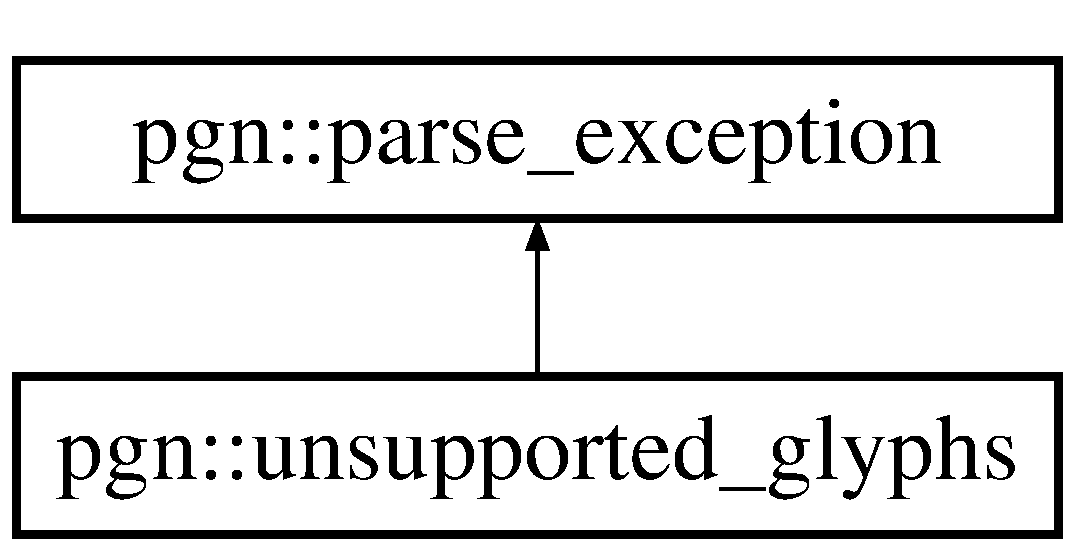
\includegraphics[height=2.000000cm]{classpgn_1_1unsupported__glyphs}
\end{center}
\end{figure}


The documentation for this class was generated from the following file:\begin{DoxyCompactItemize}
\item 
src/libpgnm/src/PGNException.h\end{DoxyCompactItemize}

\hypertarget{classpgn_1_1unsupported__variations}{
\section{pgn::unsupported\_\-variations Class Reference}
\label{classpgn_1_1unsupported__variations}\index{pgn::unsupported\_\-variations@{pgn::unsupported\_\-variations}}
}
Inheritance diagram for pgn::unsupported\_\-variations:\begin{figure}[H]
\begin{center}
\leavevmode
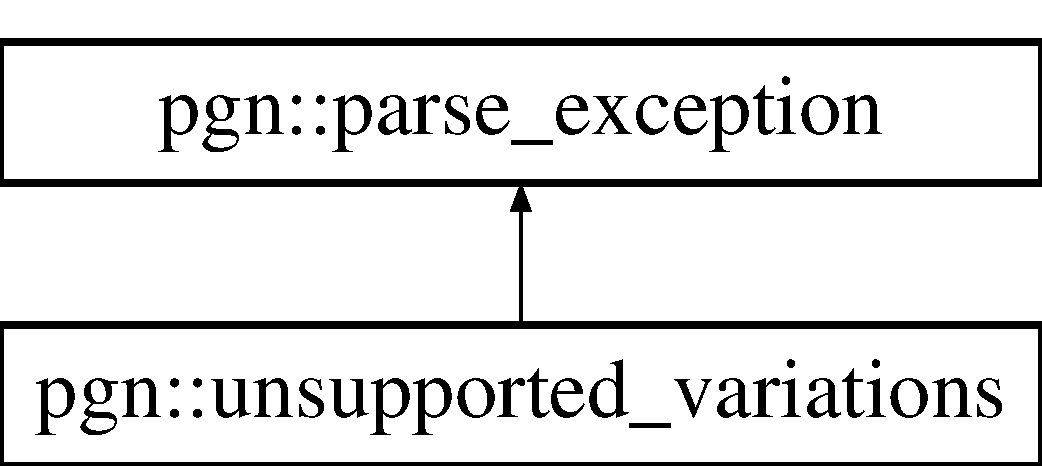
\includegraphics[height=2.000000cm]{classpgn_1_1unsupported__variations}
\end{center}
\end{figure}


The documentation for this class was generated from the following file:\begin{DoxyCompactItemize}
\item 
src/libpgnm/src/PGNException.h\end{DoxyCompactItemize}

\chapter{File Documentation}
\hypertarget{CEEngine_8h}{
\section{src/CEEngine.h File Reference}
\label{CEEngine_8h}\index{src/CEEngine.h@{src/CEEngine.h}}
}
{\ttfamily \#include \char`\"{}CETable.h\char`\"{}}\par
{\ttfamily \#include $<$PGNGame.h$>$}\par
{\ttfamily \#include $<$PGNMoveList.h$>$}\par
{\ttfamily \#include $<$PGNPly.h$>$}\par
{\ttfamily \#include $<$iostream$>$}\par
\subsection*{Classes}
\begin{DoxyCompactItemize}
\item 
class \hyperlink{classChEngn_1_1Engine}{ChEngn::Engine}
\begin{DoxyCompactList}\small\item\em Make moves. \item\end{DoxyCompactList}\end{DoxyCompactItemize}
\subsection*{Namespaces}
\begin{DoxyCompactItemize}
\item 
namespace \hyperlink{namespaceChEngn}{ChEngn}


\begin{DoxyCompactList}\small\item\em Contains all typedefs, constants, classes defined in. \item\end{DoxyCompactList}

\end{DoxyCompactItemize}
\subsection*{Typedefs}
\begin{DoxyCompactItemize}
\item 
typedef \hyperlink{classChEngn_1_1Table}{ChEngn::Table} \hyperlink{namespaceChEngn_a5ba229504d25ed1b2086f1df62f6db41}{ChEngn::VirtualTable}
\end{DoxyCompactItemize}


\subsection{Detailed Description}
Provides access to current game. Can make moves, get table state ( Virtual Table)

\begin{DoxyNote}{Note}
This class {\bfseries does not} manipulate pgn files. 
\end{DoxyNote}

\hypertarget{CEEnumerator_8h}{
\section{src/CEEnumerator.h File Reference}
\label{CEEnumerator_8h}\index{src/CEEnumerator.h@{src/CEEnumerator.h}}
}


Here defined ChEngn::Enumetaror class.  


{\ttfamily \#include $<$iostream$>$}\par
{\ttfamily \#include $<$CETable.h$>$}\par
{\ttfamily \#include $<$CEPiece.h$>$}\par
\subsection*{Classes}
\begin{DoxyCompactItemize}
\item 
class \hyperlink{classChEngn_1_1Enumerator}{ChEngn::Enumerator}
\begin{DoxyCompactList}\small\item\em \hyperlink{classChEngn_1_1Enumerator}{Enumerator} possibilites. \item\end{DoxyCompactList}\end{DoxyCompactItemize}
\subsection*{Namespaces}
\begin{DoxyCompactItemize}
\item 
namespace \hyperlink{namespaceChEngn}{ChEngn}


\begin{DoxyCompactList}\small\item\em Contains all typedefs, constants, classes defined in. \item\end{DoxyCompactList}

\end{DoxyCompactItemize}
\subsection*{Enumerations}
\begin{DoxyCompactItemize}
\item 
enum \hyperlink{namespaceChEngn_a680bcca190861d8cee0f8627ce8f9de3}{ChEngn::EnumerationSide} \{ {\bfseries UndefinedSide} =  0, 
\hyperlink{namespaceChEngn_a680bcca190861d8cee0f8627ce8f9de3a1216fa4a94b6a39e924f5965c2f077c8}{ChEngn::WhiteSide}, 
\hyperlink{namespaceChEngn_a680bcca190861d8cee0f8627ce8f9de3a957467874ae046942182f37a5dd95cf1}{ChEngn::BlackSide}
 \}
\end{DoxyCompactItemize}


\subsection{Detailed Description}
Here defined ChEngn::Enumetaror class. 
\hypertarget{CEException_8h}{
\section{src/CEException.h File Reference}
\label{CEException_8h}\index{src/CEException.h@{src/CEException.h}}
}


Here are defined \hyperlink{classChEngn_1_1Exception}{ChEngn::Exception} class.  


{\ttfamily \#include $<$string$>$}\par
{\ttfamily \#include $<$exception$>$}\par
\subsection*{Classes}
\begin{DoxyCompactItemize}
\item 
class \hyperlink{classChEngn_1_1Exception}{ChEngn::Exception}
\end{DoxyCompactItemize}
\subsection*{Namespaces}
\begin{DoxyCompactItemize}
\item 
namespace \hyperlink{namespaceChEngn}{ChEngn}


\begin{DoxyCompactList}\small\item\em Contains all typedefs, constants, classes defined in. \item\end{DoxyCompactList}

\end{DoxyCompactItemize}
\subsection*{Typedefs}
\begin{DoxyCompactItemize}
\item 
typedef int \hyperlink{namespaceChEngn_a347ab4e4a29f725ed0253d8311c82233}{ChEngn::ERROR\_\-CODE}
\item 
\hypertarget{namespaceChEngn_a01b85c98a5b00144710f14c2e5c11656}{
typedef std::string \hyperlink{namespaceChEngn_a01b85c98a5b00144710f14c2e5c11656}{ChEngn::ERROR\_\-MSG}}
\label{namespaceChEngn_a01b85c98a5b00144710f14c2e5c11656}

\begin{DoxyCompactList}\small\item\em ERROR\_\-MSG Empty typedef for nice code :) \item\end{DoxyCompactList}\end{DoxyCompactItemize}
\subsection*{Variables}
\begin{DoxyCompactItemize}
\item 
\hypertarget{namespaceChEngn_a58f231c1008467b4b6cfb17b190293a5}{
const int \hyperlink{namespaceChEngn_a58f231c1008467b4b6cfb17b190293a5}{ChEngn::OK\_\-I} = 0}
\label{namespaceChEngn_a58f231c1008467b4b6cfb17b190293a5}

\begin{DoxyCompactList}\small\item\em Useless code, used as deafult value, for example in copy-\/constructor. \item\end{DoxyCompactList}\item 
\hypertarget{namespaceChEngn_a36e55f6e51b01a42dd9f96ee00ea449f}{
const int \hyperlink{namespaceChEngn_a36e55f6e51b01a42dd9f96ee00ea449f}{ChEngn::CAN\_\-T\_\-FIND\_\-SOURCE\_\-PIECE\_\-I} = -\/1}
\label{namespaceChEngn_a36e55f6e51b01a42dd9f96ee00ea449f}

\begin{DoxyCompactList}\small\item\em Used when \hyperlink{classChEngn_1_1Engine}{ChEngn::Engine} tryes to make ply, but can't find piece which has been moved. \item\end{DoxyCompactList}\item 
\hypertarget{namespaceChEngn_ac4cbfc0117c3f4f03371093971bd2a52}{
const int \hyperlink{namespaceChEngn_ac4cbfc0117c3f4f03371093971bd2a52}{ChEngn::CAN\_\-T\_\-FIND\_\-DESTINATION\_\-PIECE\_\-I} = -\/2}
\label{namespaceChEngn_ac4cbfc0117c3f4f03371093971bd2a52}

\begin{DoxyCompactList}\small\item\em Used when \hyperlink{classChEngn_1_1Engine}{ChEngn::Engine} tryes to make ply, but can't find destination piece. \item\end{DoxyCompactList}\item 
\hypertarget{namespaceChEngn_afa7a66c1b6f627c2188c24575c8b07ac}{
const int \hyperlink{namespaceChEngn_afa7a66c1b6f627c2188c24575c8b07ac}{ChEngn::CAN\_\-T\_\-MAKE\_\-CASTLING\_\-I} = -\/3}
\label{namespaceChEngn_afa7a66c1b6f627c2188c24575c8b07ac}

\begin{DoxyCompactList}\small\item\em Used when castling can't be do. Chech chess rules for cases when this exception can be used. \item\end{DoxyCompactList}\item 
\hypertarget{namespaceChEngn_a6760a84e5ef9de4cb6c0e7158965d51c}{
const int \hyperlink{namespaceChEngn_a6760a84e5ef9de4cb6c0e7158965d51c}{ChEngn::PLY\_\-S\_\-POINTER\_\-IS\_\-NULL\_\-I} = -\/4}
\label{namespaceChEngn_a6760a84e5ef9de4cb6c0e7158965d51c}

\begin{DoxyCompactList}\small\item\em Used when ply pointer given to ChEngn::Engine::make$<$PieceType$>$Ply is equal to 0. \item\end{DoxyCompactList}\item 
\hypertarget{namespaceChEngn_a1afece927fee62ec6ba3fc3f600db014}{
const int \hyperlink{namespaceChEngn_a1afece927fee62ec6ba3fc3f600db014}{ChEngn::OUT\_\-OF\_\-RANGE\_\-I} = -\/5}
\label{namespaceChEngn_a1afece927fee62ec6ba3fc3f600db014}

\begin{DoxyCompactList}\small\item\em Used when uses tryes to get access to whong piece from \hyperlink{classChEngn_1_1Table}{ChEngn::Table}. \item\end{DoxyCompactList}\item 
\hypertarget{namespaceChEngn_a669b96f20597d4a0b00d4c9e4db68ee8}{
const std::string \hyperlink{namespaceChEngn_a669b96f20597d4a0b00d4c9e4db68ee8}{ChEngn::OK\_\-S} = \char`\"{}Everything is ok\char`\"{}}
\label{namespaceChEngn_a669b96f20597d4a0b00d4c9e4db68ee8}

\begin{DoxyCompactList}\small\item\em Useles message. \item\end{DoxyCompactList}\item 
\hypertarget{namespaceChEngn_afcb9219c354a7e8e1374e15cd5be767f}{
const std::string \hyperlink{namespaceChEngn_afcb9219c354a7e8e1374e15cd5be767f}{ChEngn::CAN\_\-T\_\-FIND\_\-SOURCE\_\-PIECE\_\-S} = \char`\"{}Can't find source piece\char`\"{}}
\label{namespaceChEngn_afcb9219c354a7e8e1374e15cd5be767f}

\begin{DoxyCompactList}\small\item\em Uses when \hyperlink{classChEngn_1_1Engine}{ChEngn::Engine} can't find piece which can make give move. \item\end{DoxyCompactList}\item 
\hypertarget{namespaceChEngn_a8bc85688808005c9d9c49aa2474809d1}{
const std::string \hyperlink{namespaceChEngn_a8bc85688808005c9d9c49aa2474809d1}{ChEngn::CAN\_\-T\_\-FIND\_\-DESTINATION\_\-PIECE\_\-S} = \char`\"{}Can't find destination piece\char`\"{}}
\label{namespaceChEngn_a8bc85688808005c9d9c49aa2474809d1}

\begin{DoxyCompactList}\small\item\em Uses when \hyperlink{classChEngn_1_1Engine}{ChEngn::Engine} can't find piece where move destination. \item\end{DoxyCompactList}\item 
\hypertarget{namespaceChEngn_afbdf882021d19396728801e116518dac}{
const std::string \hyperlink{namespaceChEngn_afbdf882021d19396728801e116518dac}{ChEngn::PLY\_\-S\_\-POINTER\_\-IS\_\-NULL\_\-S} = \char`\"{}Given Ply's pointer is == 0\char`\"{}}
\label{namespaceChEngn_afbdf882021d19396728801e116518dac}

\begin{DoxyCompactList}\small\item\em Used when ply pointer given to ChEngn::Engine::make$<$PieceType$>$Ply is equal to 0. \item\end{DoxyCompactList}\item 
\hypertarget{namespaceChEngn_a0c588cbbd7367bc19a844ea5966686f5}{
const std::string \hyperlink{namespaceChEngn_a0c588cbbd7367bc19a844ea5966686f5}{ChEngn::OUT\_\-OF\_\-RANGE\_\-S} = \char`\"{}Trying to acces bad position in table\char`\"{}}
\label{namespaceChEngn_a0c588cbbd7367bc19a844ea5966686f5}

\begin{DoxyCompactList}\small\item\em Used when uses tryes to get access to whong piece from \hyperlink{classChEngn_1_1Table}{ChEngn::Table}. \item\end{DoxyCompactList}\end{DoxyCompactItemize}


\subsection{Detailed Description}
Here are defined \hyperlink{classChEngn_1_1Exception}{ChEngn::Exception} class. 
\hypertarget{CEPiece_8h}{
\section{src/CEPiece.h File Reference}
\label{CEPiece_8h}\index{src/CEPiece.h@{src/CEPiece.h}}
}


Here are defined \hyperlink{classChEngn_1_1Piece}{ChEngn::Piece} class. Most of constants and structs: \hyperlink{namespaceChEngn_a491b2eba2f766087f4f28948005ab16a}{ChEngn::piece\_\-movement\_\-flag}, \hyperlink{namespaceChEngn_a9c81426c0134a97288a226c122daf62f}{ChEngn::piece\_\-color}, \hyperlink{namespaceChEngn_a2a35c185f259757a78e937575b8ed483}{ChEngn::piece\_\-type},.  


{\ttfamily \#include $<$iostream$>$}\par
\subsection*{Classes}
\begin{DoxyCompactItemize}
\item 
class \hyperlink{classChEngn_1_1Piece}{ChEngn::Piece}
\begin{DoxyCompactList}\small\item\em Chess piece. \item\end{DoxyCompactList}\end{DoxyCompactItemize}
\subsection*{Namespaces}
\begin{DoxyCompactItemize}
\item 
namespace \hyperlink{namespaceChEngn}{ChEngn}


\begin{DoxyCompactList}\small\item\em Contains all typedefs, constants, classes defined in. \item\end{DoxyCompactList}

\end{DoxyCompactItemize}
\subsection*{Typedefs}
\begin{DoxyCompactItemize}
\item 
\hypertarget{namespaceChEngn_a2a35c185f259757a78e937575b8ed483}{
typedef const unsigned char \hyperlink{namespaceChEngn_a2a35c185f259757a78e937575b8ed483}{ChEngn::piece\_\-type}}
\label{namespaceChEngn_a2a35c185f259757a78e937575b8ed483}

\begin{DoxyCompactList}\small\item\em \hyperlink{classChEngn_1_1Piece}{Piece} type is just a unsigned char. \item\end{DoxyCompactList}\item 
\hypertarget{namespaceChEngn_a9c81426c0134a97288a226c122daf62f}{
typedef const unsigned char \hyperlink{namespaceChEngn_a9c81426c0134a97288a226c122daf62f}{ChEngn::piece\_\-color}}
\label{namespaceChEngn_a9c81426c0134a97288a226c122daf62f}

\begin{DoxyCompactList}\small\item\em \hyperlink{classChEngn_1_1Piece}{Piece} color is just a unsigned char. \item\end{DoxyCompactList}\item 
\hypertarget{namespaceChEngn_a491b2eba2f766087f4f28948005ab16a}{
typedef const unsigned char \hyperlink{namespaceChEngn_a491b2eba2f766087f4f28948005ab16a}{ChEngn::piece\_\-movement\_\-flag}}
\label{namespaceChEngn_a491b2eba2f766087f4f28948005ab16a}

\begin{DoxyCompactList}\small\item\em \hyperlink{classChEngn_1_1Piece}{Piece} movement flag is just a bit in unsigned char. \item\end{DoxyCompactList}\end{DoxyCompactItemize}
\subsection*{Variables}
\begin{DoxyCompactItemize}
\item 
\hypertarget{namespaceChEngn_a538ef441c024a7e5d4c1dedb5e03fc21}{
piece\_\-type \hyperlink{namespaceChEngn_a538ef441c024a7e5d4c1dedb5e03fc21}{ChEngn::unknown} = 63}
\label{namespaceChEngn_a538ef441c024a7e5d4c1dedb5e03fc21}

\begin{DoxyCompactList}\small\item\em Uses to present unknown type piece 63 = \mbox{[}00011111\mbox{]}. \item\end{DoxyCompactList}\item 
\hypertarget{namespaceChEngn_af4781da8088272ec86e35be681dde106}{
piece\_\-type \hyperlink{namespaceChEngn_af4781da8088272ec86e35be681dde106}{ChEngn::pawn} = 1 $<$$<$ 0}
\label{namespaceChEngn_af4781da8088272ec86e35be681dde106}

\begin{DoxyCompactList}\small\item\em Uses to present pawns. \item\end{DoxyCompactList}\item 
\hypertarget{namespaceChEngn_ab167075161c66436eef6d7f02507c115}{
piece\_\-type \hyperlink{namespaceChEngn_ab167075161c66436eef6d7f02507c115}{ChEngn::knight} = 1 $<$$<$ 1}
\label{namespaceChEngn_ab167075161c66436eef6d7f02507c115}

\begin{DoxyCompactList}\small\item\em Uses to present knights. \item\end{DoxyCompactList}\item 
\hypertarget{namespaceChEngn_ad9410a19494f941d06ea404edf4900b0}{
piece\_\-type \hyperlink{namespaceChEngn_ad9410a19494f941d06ea404edf4900b0}{ChEngn::bishop} = 1 $<$$<$ 2}
\label{namespaceChEngn_ad9410a19494f941d06ea404edf4900b0}

\begin{DoxyCompactList}\small\item\em Uses to present bishops. \item\end{DoxyCompactList}\item 
\hypertarget{namespaceChEngn_a485787ab76caf7a61a77118fcdfd113d}{
piece\_\-type \hyperlink{namespaceChEngn_a485787ab76caf7a61a77118fcdfd113d}{ChEngn::rook} = 1 $<$$<$ 3}
\label{namespaceChEngn_a485787ab76caf7a61a77118fcdfd113d}

\begin{DoxyCompactList}\small\item\em Uses to present rooks. \item\end{DoxyCompactList}\item 
\hypertarget{namespaceChEngn_a97924767720e8ba4e595ad9f161d73e8}{
piece\_\-type \hyperlink{namespaceChEngn_a97924767720e8ba4e595ad9f161d73e8}{ChEngn::queen} = 1 $<$$<$ 4}
\label{namespaceChEngn_a97924767720e8ba4e595ad9f161d73e8}

\begin{DoxyCompactList}\small\item\em Uses to present queens. \item\end{DoxyCompactList}\item 
\hypertarget{namespaceChEngn_a40c2dbaf0963b46704f08ffb28364cea}{
piece\_\-type \hyperlink{namespaceChEngn_a40c2dbaf0963b46704f08ffb28364cea}{ChEngn::king} = 1 $<$$<$ 5}
\label{namespaceChEngn_a40c2dbaf0963b46704f08ffb28364cea}

\begin{DoxyCompactList}\small\item\em Uses to present kings. \item\end{DoxyCompactList}\item 
\hypertarget{namespaceChEngn_aa3212b290980eb5db7f91e88f8803a9c}{
piece\_\-color \hyperlink{namespaceChEngn_aa3212b290980eb5db7f91e88f8803a9c}{ChEngn::white} = 1 $<$$<$ 6}
\label{namespaceChEngn_aa3212b290980eb5db7f91e88f8803a9c}

\begin{DoxyCompactList}\small\item\em Uses to set flag if piece is white ( else flag is not set). \item\end{DoxyCompactList}\item 
\hypertarget{namespaceChEngn_aa2bfc6fe87969d3e28eecbb682e802c8}{
piece\_\-color \hyperlink{namespaceChEngn_aa2bfc6fe87969d3e28eecbb682e802c8}{ChEngn::black} = 0 $<$$<$ 6}
\label{namespaceChEngn_aa2bfc6fe87969d3e28eecbb682e802c8}

\begin{DoxyCompactList}\small\item\em Uses to unset flag if piece is black. \item\end{DoxyCompactList}\item 
\hypertarget{namespaceChEngn_a2997c391593541b72a894e9cf44c90bf}{
piece\_\-movement\_\-flag \hyperlink{namespaceChEngn_a2997c391593541b72a894e9cf44c90bf}{ChEngn::moved} = 1 $<$$<$ 7}
\label{namespaceChEngn_a2997c391593541b72a894e9cf44c90bf}

\begin{DoxyCompactList}\small\item\em Uses to set flag is piece has been moved. \item\end{DoxyCompactList}\end{DoxyCompactItemize}


\subsection{Detailed Description}
Here are defined \hyperlink{classChEngn_1_1Piece}{ChEngn::Piece} class. Most of constants and structs: \hyperlink{namespaceChEngn_a491b2eba2f766087f4f28948005ab16a}{ChEngn::piece\_\-movement\_\-flag}, \hyperlink{namespaceChEngn_a9c81426c0134a97288a226c122daf62f}{ChEngn::piece\_\-color}, \hyperlink{namespaceChEngn_a2a35c185f259757a78e937575b8ed483}{ChEngn::piece\_\-type},. 
\hypertarget{CETable_8h}{
\section{src/CETable.h File Reference}
\label{CETable_8h}\index{src/CETable.h@{src/CETable.h}}
}


\hyperlink{namespaceChEngn_ae87757a4f2d9ae9e25d48213cad79ddd}{ChEngn::default\_\-table\_\-height}, \hyperlink{namespaceChEngn_a9dc4a83c122aec6e170ad7a1d40efd8a}{ChEngn::default\_\-table\_\-width}.  


{\ttfamily \#include \char`\"{}CEPiece.h\char`\"{}}\par
{\ttfamily \#include $<$iostream$>$}\par
\subsection*{Classes}
\begin{DoxyCompactItemize}
\item 
class \hyperlink{classChEngn_1_1Table}{ChEngn::Table}
\begin{DoxyCompactList}\small\item\em Chess board. \item\end{DoxyCompactList}\end{DoxyCompactItemize}
\subsection*{Namespaces}
\begin{DoxyCompactItemize}
\item 
namespace \hyperlink{namespaceChEngn}{ChEngn}


\begin{DoxyCompactList}\small\item\em Contains all typedefs, constants, classes defined in. \item\end{DoxyCompactList}

\end{DoxyCompactItemize}
\subsection*{Variables}
\begin{DoxyCompactItemize}
\item 
\hypertarget{namespaceChEngn_ae87757a4f2d9ae9e25d48213cad79ddd}{
const unsigned int \hyperlink{namespaceChEngn_ae87757a4f2d9ae9e25d48213cad79ddd}{ChEngn::default\_\-table\_\-height} = 8}
\label{namespaceChEngn_ae87757a4f2d9ae9e25d48213cad79ddd}

\begin{DoxyCompactList}\small\item\em Standart table height. \item\end{DoxyCompactList}\item 
\hypertarget{namespaceChEngn_a9dc4a83c122aec6e170ad7a1d40efd8a}{
const unsigned int \hyperlink{namespaceChEngn_a9dc4a83c122aec6e170ad7a1d40efd8a}{ChEngn::default\_\-table\_\-width} = 8}
\label{namespaceChEngn_a9dc4a83c122aec6e170ad7a1d40efd8a}

\begin{DoxyCompactList}\small\item\em Standart table width. \item\end{DoxyCompactList}\end{DoxyCompactItemize}


\subsection{Detailed Description}
\hyperlink{namespaceChEngn_ae87757a4f2d9ae9e25d48213cad79ddd}{ChEngn::default\_\-table\_\-height}, \hyperlink{namespaceChEngn_a9dc4a83c122aec6e170ad7a1d40efd8a}{ChEngn::default\_\-table\_\-width}. Here defined \hyperlink{classChEngn_1_1Table}{ChEngn::Table}, ChEngn::table\_\-size, 
\hypertarget{CEUtils_8h}{
\section{src/CEUtils.h File Reference}
\label{CEUtils_8h}\index{src/CEUtils.h@{src/CEUtils.h}}
}


Here are defined ChEngn::Exception class.  


{\ttfamily \#include $<$string$>$}\par
\subsection*{Namespaces}
\begin{DoxyCompactItemize}
\item 
namespace \hyperlink{namespaceChEngn}{ChEngn}


\begin{DoxyCompactList}\small\item\em Contains all typedefs, constants, classes defined in. \item\end{DoxyCompactList}

\end{DoxyCompactItemize}
\subsection*{Functions}
\begin{DoxyCompactItemize}
\item 
std::string \hyperlink{namespaceChEngn_a5d21d3814a89e92e086273036613ce2f}{ChEngn::itostr} (int num)
\begin{DoxyCompactList}\small\item\em Converts given number to std::string. \item\end{DoxyCompactList}\item 
const char $\ast$ \hyperlink{namespaceChEngn_ade01056f903a4bcf3606ca380be66d0a}{ChEngn::itoa} (int num)
\begin{DoxyCompactList}\small\item\em Converts given number to std::string. \item\end{DoxyCompactList}\end{DoxyCompactItemize}


\subsection{Detailed Description}
Here are defined ChEngn::Exception class. 
\chapter{Example Documentation}
\hypertarget{examples_2main_8cpp-example}{
\section{examples/main.cpp}
}
First exampleThis example shows howto open pgn file and make all moves for each game from file.

Compile and run:

\$ make 

\$ make run


\begin{DoxyCodeInclude}
#include <iostream>
#include <PGNFile.h>
#include <CEEngine.h>
#include <CEException.h>

int main()
{
    pgn::File file( "myfile.pgn" );
    
    for ( int i = 0; i < file.games().size(); i ++ )
    {
        ChEngn::Engine engine( file.games()[ i ] );
        try {
            while( engine.makeNextHalfMove() )
            {
                ;
            }
        }
        catch ( ChEngn::BadMove e )
        {
            std::cerr << e.what() << std::endl;
        }
        catch( ... )
        {
            std::cerr << "Unknown error..." << std::endl;
        }
    }

    return 0;
}
\end{DoxyCodeInclude}
 
\printindex
\end{document}
